% -------------------------------------------------------------------------------------------------
%      MDSG Latex Framework
%      ============================================================================================
%      File:                  main.tex
%      Author(s):             Michael Duerr
%      Version:               1
%      Creation Date:         30. Mai 2010
%      Creation Date:         30. Mai 2010
%
%      Notes:                 - This represents the document root of this template
%                             - Binding correction is 12mm. In case you change this value, you
%                               may also need to adapt the value of \bcorlength in mdsg.sty
%                             - Switch `babel' package options `english' and `ngerman' in case
%                               your thesis is in English
%                             - if you prefer to use utf8 encoding, uncomment the corresponding
%                               line `\usepackage[utf8]{inputenc}' and comment the line
%                               `\usepackage[latin1]{inputenc}'. To compile this example you also
%                               need to include the corresponding introduction example file i.e.
%                               `introduction-UTF8.tex' or `introduction-ISO8859-1.tex'
% -------------------------------------------------------------------------------------------------
%
\documentclass[enabledeprecatedfontcommands,bibliography=totoc,listof=totoc,index=totoc,twoside=true,BCOR=12mm,DIV=12]{scrbook} % TODO evtl ändern
%\KOMAoptions{draft=true}                         % uncomment if you want to visualise overful hbox
%\KOMAoptions{chapterprefix=true}                 % uncomment if you like "Chapter" in front of
                                                  % chapter number
%\KOMAoptions{appendixprefix=true}                % uncomment if you like "Appendix" in front of
                                                  % appendix number
%\KOMAoptions{...}                                % feel free to add additional KOMA options
%
% =================================================================================================
% set encoding
% -------------------------------------------------------------------------------------------------
%
\usepackage[utf8]{inputenc}                       % uncomment if you prefer utf8 encoding
%\usepackage[latin1]{inputenc}                    % uncomment if you prefer latin1 encoding
%
% =================================================================================================
% load mdsg style
% -------------------------------------------------------------------------------------------------
%
%\usepackage[diplom]{mdsg}                        % uncomment the corresponding option
%\usepackage[fopra]{mdsg}
\usepackage[bachelor]{mdsg}
%\usepackage[master]{mdsg}
%
% =================================================================================================
% initialize macros
% -------------------------------------------------------------------------------------------------
%
% \lmutitle{Representing algorithmic properties of learning algorithms within their reward function}                       % title: you can force a new line by
\lmutitle{Abbildung von Learning-Algorithmen-Modellen in deren Reward-Funktion}
%\lmutitle{Titel \\ der \\ Arbeit}                % inserting `\\'. However, this will cause
                                                  % a hyperref warning!
\lmustudentone{David Müller}                    % first author's name
%\lmustudenttwo{Max2 Mustermann2}                 % second author's name
%\lmustudentthree{Max3 Mustermann3}               % third author's name
%\lmustudentfour{Max4 Mustermann4}                % fourth author's name

\lmuprofone{Prof. Dr. Claudia Linnhoff-Popien}    % first supervisor's name
% \lmuproftwo{Prof. Dr. Max Mustermann}             % second supervisor's name
                                                  % (uncomment if not needed)
% \lmuprofthree{Prof. Dr. Max2 Mustermann2}         % third supervisor's name
                                                  % (uncomment if not needed)
\lmuadvisorone{Thomas Gabor}                    % first advisor's name
\lmuadvisortwo{Thomy Phan}                    % second advisor's name
                                                  % (uncomment if not needed)
% \lmuadvisorthree{Betreuer Name3}                  % third advisor's name
                                                  % (uncomment if not needed)
\lmudraftdate{\today}                             % only for versioning during work!
                                                  % (uncomment for final version!)
\lmudeadline{1. Januar 2099}                      % deadline (day of submission)
%
% =================================================================================================
% package selection (add additional packages if needed)
% -------------------------------------------------------------------------------------------------
%
%\usepackage{layout}                              % see documentation of this package
\usepackage{cmap}                                 % to produce searchable PDF
\usepackage[T1]{fontenc}                          % split german words with umlaut
\usepackage{lmodern}
\usepackage[english,ngerman]{babel}               % for german toc, ...
\usepackage{bibgerm}                              % for german bibliography index
\usepackage{tabularx}                             % more flexible table environment
\usepackage{booktabs}                             % high quality tables
\usepackage{rotating}                             % for generation of landscape tables
\usepackage{multirow}                             % for multirow cells inside tables
\usepackage{amssymb,amsmath}                      % powerful math package
\usepackage{hyperref}                             % for hyperlinks
\lmuhypersetup                                    % write some pdf properties
\usepackage{flafter}                              % force floats to appear after their reference
% \usepackage{subfig}                               % to allow for side by side graphics (subfloats)
\usepackage{pdflscape}                            % enable rotation of landscape pages
\usepackage{hyphenat}                             % proper hyphenation for bla_bla to bla_-bla
\usepackage[all]{hypcap}                          % correct captions
\usepackage{url}                                  % nicer url style
\usepackage{enumitem}                             % for tight lists
\usepackage{minted}
\usepackage{graphicx}
\usepackage{caption}
\usepackage{subcaption}
\usepackage{mdwlist}
\usepackage{xurl}

\setcounter{tocdepth}{3}                          % sectioning depth in toc
\setcounter{secnumdepth}{3}                       % sectioning depth in text

\graphicspath{{./pictures/}}                      % put all graphics here
% -------------------------------------------------------------------------------------------------
%      MDSG Latex Framework
%      ============================================================================================
%      File:                  hyphenation.tex
%      Author(s):             Michael Duerr
%      Version:               1
%      Creation Date:         30. Mai 2010
%      Creation Date:         30. Mai 2010
%
%      Notes:                 - Instruction \hypenation cannot handle special characters like umlaute
%                               as well as  "a and \"a. Split such words in your text.
%
% -------------------------------------------------------------------------------------------------
%
\hyphenation{Ba-che-lor-ar-}
%\hyphenation{...}                           % further hyphenation examples
                               % this file holds words latex cannot split
%
% =================================================================================================
% start of document
% -------------------------------------------------------------------------------------------------
%
\begin{document}
    \newcommand{\smallspace}{\vspace{4mm}}
\newcommand{\bigspace}{\vspace{7mm}}
\newcommand{\source}[1]{\caption*{\footnotesize Quelle: {#1}}}

% \usemintedstyle{perldoc}
\usemintedstyle{autumn}
% \usemintedstyle{pastie}

\newenvironment{code}{\captionsetup{type=listing}}{}
    \setlist{noitemsep}                           % for tight lists
    \lmufront                                     % title pages
    \newpage
    \cleardoublepage
    \lmuaffirmation                               % affirmation (work is my own work)
    \newpage
    \cleardoubleemptypage
    \thispagestyle{empty}
    % -------------------------------------------------------------------------------------------------
%      MDSG Latex Framework
%      ============================================================================================
%      File:                  abstract.tex
%      Author(s):             Michael Duerr
%      Version:               1
%      Creation Date:         30. Mai 2010
%      Creation Date:         30. Mai 2010
%
%      Notes:                 - Place your abstract here
% -------------------------------------------------------------------------------------------------
%
\vspace*{2cm}

\begin{center}
    \textbf{Abstract}
\end{center}

\vspace*{1cm}

% \noindent Learning-Algorithmen nutzen eine Vielzahl von Modellen und Strategien, um das Lernverhalten des Agenten zu kontrollieren und dessen Resultate zu verbessern. Wir untersuchen, inwieweit sich diese in der Reward-Funktion abbilden lassen und welche Auswirkungen dies auf das Lernverhalten sowie die Resultate des Agents hat. Außerdem analysieren wir, welchem Ziel der Algorithmus mit der Reward-Funktion tatsächlich folgt und stellen dies anschaulich dar. Zu diesem Zweck wird ein Landschaftsnavigationsproblem betrachtet, in dem der Agent in einem zufällig generierten Terrain den höchsten Gipfel finden soll.

\noindent Für Machine-Learning-Algorithmen gibt es eine Vielzahl von Modellen und Strategien, die genutzt werden können, um das Lernverhalten des Agenten zu kontrollieren und damit schlussendlich dessen Resultate zu verbessern. Bereits eine simple Erweiterung wie das Lernen auf einer Epsilon-Greedy-Policy fügt so schon neue Komponenten zum Lernalgorithmus hinzu. Wir untersuchen, inwieweit sich derartige Erweiterungen allein durch die Wahl der Reward-Funktion abbilden lassen und welche Auswirkungen dies auf das Lernverhalten sowie die Resultate des Agenten hat. Außerdem wird in diesem Zuge analysiert, welches eigentliche Ziel durch so eine Reward-Funktion umgesetzt wird. Für eine anschauliche Darstellung wird ein Landschaftsnavigationsproblem betrachtet, in dem der Agent in einem zufällig generierten Terrain den höchsten Gipfel finden soll.

% abbilden in der reward-Funktion 
% was ist die echte reward funktion 
                       % abstract
    \thispagestyle{empty}
    \frontmatter                                  % start roman numbering
    \tableofcontents                              % toc
    \mainmatter                                   % start alpha numbering
%
% =================================================================================================
% place your document text here (take care of encoding)
% -------------------------------------------------------------------------------------------------
%
    % % -------------------------------------------------------------------------------------------------
%      MDSG Latex Framework
%      ============================================================================================
%      File:                  introduction-[UTF8,ISO8859-1].tex
%      Author(s):             Michael Duerr
%      Version:               1
%      Creation Date:         30. Mai 2010
%      Creation Date:         30. Mai 2010
%
%      Notes:                 - Example chapter
% -------------------------------------------------------------------------------------------------
%
\chapter{Einleitung}\label{sec:Introduction}
Dies ist der \LaTeX\ Rahmen zur Bearbeitung von Bachelor-, Master-, Projekt- und Diplomarbeiten.
Alle relevanten Dateien befinden sich im Verzeichnis \verb|text|.
\section{Unterverzeichnisse und Dateien}
Das Verzeichnis \verb|text| beinhaltet weitere Unterverzeichnisse und Dateien, die den Rahmen charakterisieren.
\subsection{\textbf{main.tex}}\label{subsec:main}
Diese Datei stellt die zentrale Konfigurationsdatei für den Rahmen dar. Unter anderem müssen hier Informationen
über die Aufgabensteller, Betreuer, die Art der Arbeit sowie deren Title eingestellt werden.
Hier können auch weitere Pakete eingebunden werden. Die Datei ist dokumentiert und sollte selbsterklärend
sein.
\subsection{\textbf{hyphenation.tex}}
Manche Wörter werden von \LaTeX\ nicht (ordentlich) getrennt. Diese können in dieser Datei mit deren
Trennungsstellen hinzugefügt werden.
\subsection{\textbf{Makefile}}
Um das Dokument zu erstellen muss man den Aufruf \verb|make all| tätigen. Dabei werden einige temporäre
Dateien erstellt sowie die Datei \verb|main.pdf| die das entsprechende Dokument enthält. Mir dem
Aufruf \verb|make clean| werden alle temporären Dateien sowie die Datei \verb|main.pdf| gelöscht.
sie können die Datei \verb|Makefile| ihren Anforderungen entsprechend erweitern.
\subsection{\textbf{text}}
Es bietet sich an für verschiedene Kapitel eigene Quelldateien zu pflegen. Diese sollten sie alle im
Ordner \verb|text| ablegen. Wie ein Kapitel eingebunden wird, kann man aus dem Beispiel in der
Datei \verb|main.tex| ablesen. Das Verzeichnis \textbf{text} beinhaltet zudem die Datei
\verb|abstract.tex|. In diese Datei soll eine kurze Zusammenfassung (ca. eine halbe Seite)
der Arbeit eingetragen werden. Die Datei \verb|appendix.tex| kann verwendet werden um einen
Anhang zu generieren.
\subsection{\textbf{pictures}}
Hier müssen sie alle Grafiken ablegen, die sie in ihrem Dokument einbinden wollen. Es sind nur die
Formate PDF, PNG und JPEG erlaubt (GIF ist möglich, wird aber nicht empfohlen).
\subsection{\textbf{bibliography.bib}}
In diese Datei müssen alle Referenzen eingetragen werden,
die innerhalb ihrer Arbeit zitiert werden. Verwenden sie zur Verwaltung ihrer Referenzen einen
geeigneten Editor z.B. \textit{JabRef} (\url{http://jabref.sourceforge.net/}).
\subsection{\textbf{mdsg.sty}}
Hierbei handelt es sich um das Stylefile, das das Erscheinungsbild des Dokuments
lenkt. In dieser Datei sollten in der Regel keine Veränderungen notwendig sein.
\section{Beispiele}
Es gibt eine Unmenge an \LaTeX\ Tutorials und Dokumentationen, die guten Einstieg in das Arbeiten mit
\LaTeX\ ermöglichen. Im Folgenden werden aber ein paar undokumentierte Minimalbeispiele gegeben, die
den direkten Einstieg ermöglichen. Betrachten sie den Quelltext, um die Beispiele nachzuvollziehen.
\subsection{Zitate}
Wir zitieren hier eine Quelle von James Aspnes et al \cite{aspn07}, die in der  Datei\\
\verb|bibliography.bib|
steht.
\subsection{Listen}
Es gibt verschiedene Möglichkeiten Listen zu erstellen, z.B. ohne Nummerierung\dots
\begin{itemize}
   \item
      Das ist der erste Punkt,
      \begin{itemize}
         \item
            das der erste Unterpunkt,
         \item
            das der zweite Unterpunkt,
   \end{itemize}
   \item
      das der zweite, und
   \item
      das der dritte Punkt.
\end{itemize}
\dots oder mit Nummerierung\dots
\begin{enumerate}
   \item
      Das ist der erste Punkt,
      \begin{enumerate}
         \item
            das der erste Unterpunkt,
         \item
            das der zweite Unterpunkt,
      \end{enumerate}
   \item
      das der zweite, und
   \item
      das der dritte Punkt.
\end{enumerate}
\subsection{Referenz auf anderen Text}
Es ist auch möglich auf andere Stellen im Text z.B. Kapitel \ref{subsec:main} zu verweisen.
\subsection{Hoch- und tiefgestellter Text}
Man kann Text tiefstellen indem man \verb|\textsubscript| verwendet, z.B. ergibt
\begin{verbatim}
text\textsubscript{tiefgestellt}
\end{verbatim}
den Text text\textsubscript{tiefgestellt}.
Das selbe funktioniert mit \verb|\textsuperscript| verwendet, z.B. ergibt
\begin{verbatim}
text\textsuperscript{hochgestellt}
\end{verbatim}
text\textsuperscript{hochgestellt}
\subsection{Tabellen}
Es gibt schöne Möglichkeiten Tabellen einzubinden wie z.B. Tabelle \ref{tab:CommonParameterSettings}.
\begin{center}
\begin{table}[htbp]
{\small
\begin{center}
\begin{tabular}[center]{lrlc}
\toprule
Parameter & Value & (Unit) & Available for Chord \\
\midrule
Query timeout & 10 & seconds & $\surd$ \\
Republish timeout & 300 & seconds & $\surd$ \\ % explain this value...
Stabilize timeout & 5 & seconds & $\surd$ \\
Fix fingers timeout & 30 & seconds & $\surd$ \\
Message timeout & 1 & second & $\surd$ \\
Connect timeout & 10 & seconds & $\surd$ \\
Ping superpeer timeout & 5 & seconds & $\times$ \\
Cost-Optimality estimation timeout & 20 & seconds & $\times$ \\
Significance for change in number of superpeers & 10 & percent & $\times$ \\
Significance for change in estimations  & 10 & percent & $\times$ \\
Number of permanent superpeers & 32 & nodes & $\times$ \\
Mean number of peers & 1000 & nodes & $\surd$ \\
Mean number of lookups per hour & 60 & queries & $\surd$ \\
Mean number of shared InfoProfiles per node & 20 & & $\surd$ \\
Identifier space & 16 & bits & $\surd$ \\
Direct insertion acknowledgment & true & bool & $\times$ \\
Direct query responses & true & bool & $\times$ \\
Force query resolution & true & bool & $\surd$  \\
\bottomrule
\end{tabular}
\end{center}
} % end of tiny
\caption[Simulation parameter settings]{Common simulation parameter settings.\label{tab:CommonParameterSettings}}
\end{table}
\end{center}

\subsection{Bilder}
Man kann sehr einfach Bilder einbinden so wie z.B. in Abbildung \ref{fig:pic0}.
\begin{figure}[hpbt]
  \centering
  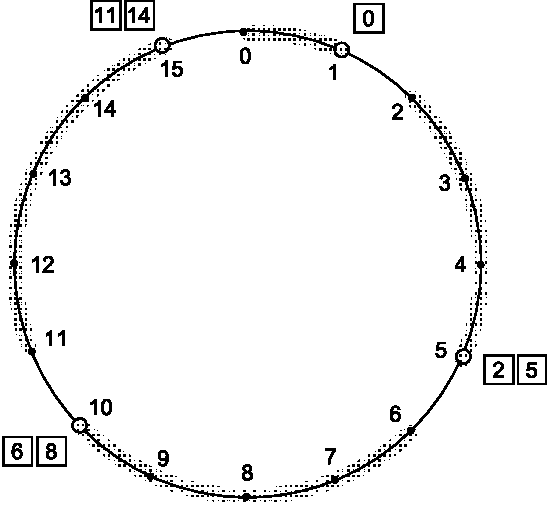
\includegraphics[width=0.4\textwidth]{pictures/pic0}\\
  \caption[Example of a $4$-bit Chord identifier circle]{Example of a $4$-bit Chord identifier circle.
  The responsibility ranges for each peer are accentuated in light gray}\label{fig:pic0}
\end{figure}
Es lassen sich auch mehrere Bilder nebeneinander platzieren wie z.B. in Abbildung
\ref{fig:multipic} zu sehen ist.
\begin{figure}[hpbt]
 \centering
  %%----start of first subfigure----
  \subfloat[FIFO size limited to 20 entries]{
   \label{fig:multipic:a} %% label for first subfigure
   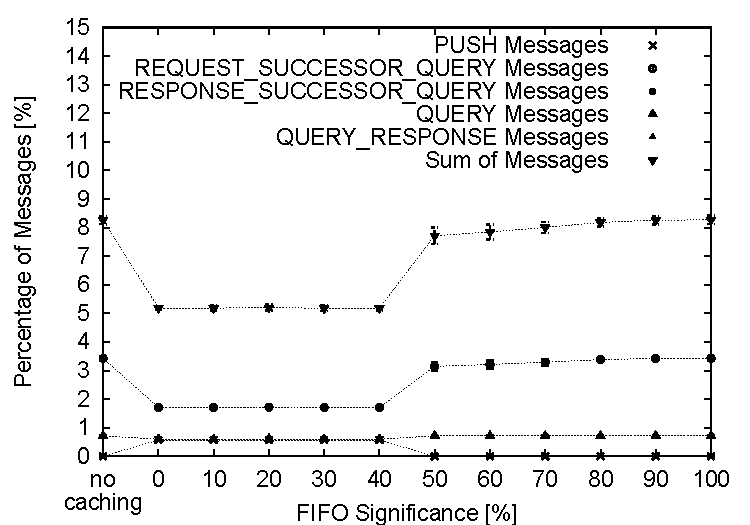
\includegraphics[width=0.48\linewidth]{pic1}}
  \hspace{0.01\textwidth}
  %%----start of second subfigure----
  \subfloat[FIFO size limited to 30 entries]{
   \label{fig:multipic:b} %% label for second subfigure
   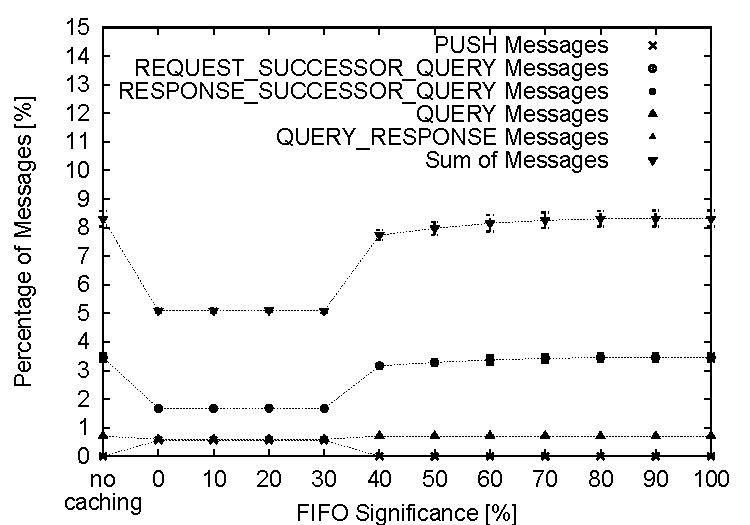
\includegraphics[width=0.48\linewidth]{pic2}}\\[0pt] % horizontal break
  %%----start of third subfigure----
  \subfloat[FIFO size limited to 40 entries]{
   \label{fig:multipic:c} %% label for third subfigure
   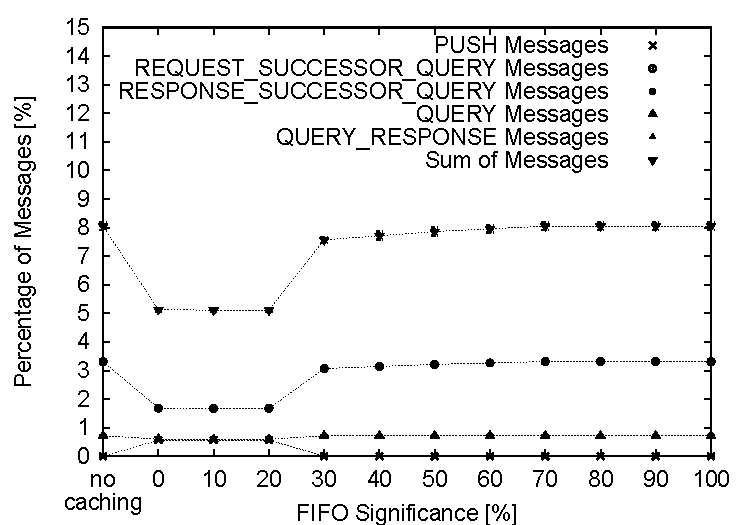
\includegraphics[width=0.48\linewidth]{pic3}}
  \hspace{0.01\textwidth}
  %%----start of fourth subfigure----
  \subfloat[FIFO size limited to 50 entries]{
   \label{fig:multipic:d} %% label for fourth subfigure
   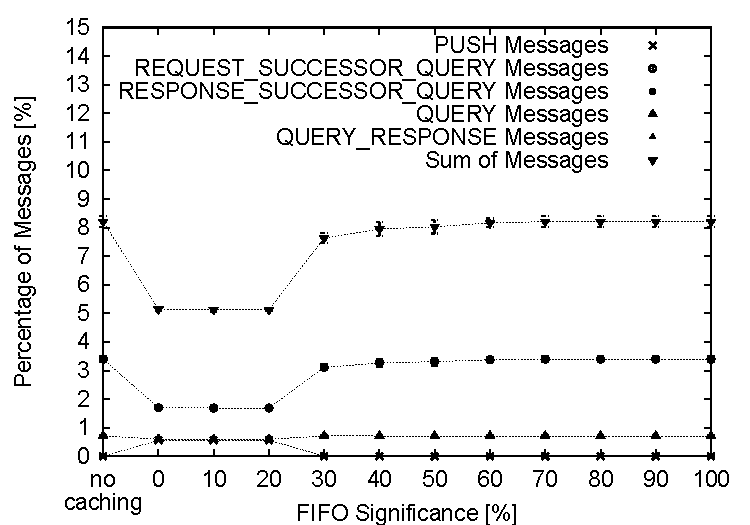
\includegraphics[width=0.48\linewidth]{pic4}}
 \caption[Observed message fractions and 95\% confidence intervals for Chord]{Observed message fractions and 95\% confidence intervals for Chord without the influence of churn. The FIFO capacity varies from 20 (\ref{fig:multipic:a}) -- 50 (\ref{fig:multipic:d}) entries (decadic steps).}
 \label{fig:multipic} %% label for entire figure
\end{figure}

\subsection{Programm Code}
Eine elegante Möglichkeit, Programmtext einzubinden, lässt sich mit dem listings-Paket erreichen.
Das \verb|HelloWorld| Programm aus Listing \ref{lst:hw} hat in Zeile \ref{line:hw3} übrigens einen Programmierfehler.
\begin{lstlisting}[float=htp,caption=Hello World,label=lst:hw,language=Java, numbers=left, numberstyle=\tiny, stepnumber=2, numbersep=8pt, escapeinside={//@}{@//},backgroundcolor=\color{yellow},xleftmargin=3ex,xrightmargin=1ex]
public class HelloWorld {
    public static void main(String[] args) {
        Syste.out.println("Hello, World"); //@\label{line:hw3}@//
    }
}
\end{lstlisting}

\subsection{Fußnoten}
Wenn man auf Google \footnote{\url{http://www.google.com}} verweisen will, bietet sich statt einer gesonderten
Referenz auch einfach eine Fußnote an.
\subsection{Formeln}
Man kann mit \LaTeX\ sehr schön Formeln erzeugen:
$$L_{P}(k) = R^{orig}_{P}(k) + \sum_{i=0}^n 2*R^{i}_{P}(k)$$

    % % -------------------------------------------------------------------------------------------------
%      MDSG Latex Framework
%      ============================================================================================
%      File:                  introduction-[UTF8,ISO8859-1].tex
%      Author(s):             Michael Duerr
%      Version:               1
%      Creation Date:         30. Mai 2010
%      Creation Date:         30. Mai 2010
%
%      Notes:                 - Example chapter
% -------------------------------------------------------------------------------------------------
%
\chapter{Einleitung}\label{sec:Introduction}
Dies ist der \LaTeX\ Rahmen zur Bearbeitung von Bachelor-, Master-, Projekt- und Diplomarbeiten.
Alle relevanten Dateien befinden sich im Verzeichnis \verb|text|.
\section{Unterverzeichnisse und Dateien}
Das Verzeichnis \verb|text| beinhaltet weitere Unterverzeichnisse und Dateien, die den Rahmen charakterisieren.
\subsection{\textbf{main.tex}}\label{subsec:main}
Diese Datei stellt die zentrale Konfigurationsdatei f�r den Rahmen dar. Unter anderem m�ssen hier Informationen
�ber die Aufgabensteller, Betreuer, die Art der Arbeit sowie deren Title eingestellt werden.
Hier k�nnen auch weitere Pakete eingebunden werden. Die Datei ist dokumentiert und sollte selbsterkl�rend
sein.
\subsection{\textbf{hyphenation.tex}}
Manche W�rter werden von \LaTeX\ nicht (ordentlich) getrennt. Diese k�nnen in dieser Datei mit deren
Trennungsstellen hinzugef�gt werden.
\subsection{\textbf{Makefile}}
Um das Dokument zu erstellen muss man den Aufruf \verb|make all| t�tigen. Dabei werden einige tempor�re
Dateien erstellt sowie die Datei \verb|main.pdf| die das entsprechende Dokument enth�lt. Mir dem
Aufruf \verb|make clean| werden alle tempor�ren Dateien sowie die Datei \verb|main.pdf| gel�scht.
sie k�nnen die Datei \verb|Makefile| ihren Anforderungen entsprechend erweitern.
\subsection{\textbf{text}}
Es bietet sich an f�r verschiedene Kapitel eigene Quelldateien zu pflegen. Diese sollten sie alle im
Ordner \verb|text| ablegen. Wie ein Kapitel eingebunden wird, kann man aus dem Beispiel in der
Datei \verb|main.tex| ablesen. Das Verzeichnis \textbf{text} beinhaltet zudem die Datei
\verb|abstract.tex|. In diese Datei soll eine kurze Zusammenfassung (ca. eine halbe Seite)
der Arbeit eingetragen werden. Die Datei \verb|appendix.tex| kann verwendet werden um einen
Anhang zu generieren.
\subsection{\textbf{pictures}}
Hier m�ssen sie alle Grafiken ablegen, die sie in ihrem Dokument einbinden wollen. Es sind nur die
Formate PDF, PNG und JPEG erlaubt (GIF ist m�glich, wird aber nicht empfohlen).
\subsection{\textbf{bibliography.bib}}
In diese Datei m�ssen alle Referenzen eingetragen werden,
die innerhalb ihrer Arbeit zitiert werden. Verwenden sie zur Verwaltung ihrer Referenzen einen
geeigneten Editor z.B. \textit{JabRef} (\url{http://jabref.sourceforge.net/}).
\subsection{\textbf{mdsg.sty}}
Hierbei handelt es sich um das Stylefile, das das Erscheinungsbild des Dokuments
lenkt. In dieser Datei sollten in der Regel keine Ver�nderungen notwendig sein.
\section{Beispiele}
Es gibt eine Unmenge an \LaTeX\ Tutorials und Dokumentationen, die guten Einstieg in das Arbeiten mit
\LaTeX\ erm�glichen. Im Folgenden werden aber ein paar undokumentierte Minimalbeispiele gegeben, die
den direkten Einstieg erm�glichen. Betrachten sie den Quelltext, um die Beispiele nachzuvollziehen.
\subsection{Zitate}
Wir zitieren hier eine Quelle von James Aspnes et al \cite{aspn07}, die in der  Datei\\
\verb|bibliography.bib|
steht.
\subsection{Listen}
Es gibt verschiedene M�glichkeiten Listen zu erstellen, z.B. ohne Nummerierung\dots
\begin{itemize}
   \item
      Das ist der erste Punkt,
      \begin{itemize}
         \item
            das der erste Unterpunkt,
         \item
            das der zweite Unterpunkt,
   \end{itemize}
   \item
      das der zweite, und
   \item
      das der dritte Punkt.
\end{itemize}
\dots oder mit Nummerierung\dots
\begin{enumerate}
   \item
      Das ist der erste Punkt,
      \begin{enumerate}
         \item
            das der erste Unterpunkt,
         \item
            das der zweite Unterpunkt,
      \end{enumerate}
   \item
      das der zweite, und
   \item
      das der dritte Punkt.
\end{enumerate}
\subsection{Referenz auf anderen Text}
Es ist auch m�glich auf andere Stellen im Text z.B. Kapitel \ref{subsec:main} zu verweisen.
\subsection{Hoch- und tiefgestellter Text}
Man kann Text tiefstellen indem man \verb|\textsubscript| verwendet, z.B. ergibt
\begin{verbatim}
text\textsubscript{tiefgestellt}
\end{verbatim}
den Text text\textsubscript{tiefgestellt}.
Das selbe funktioniert mit \verb|\textsuperscript| verwendet, z.B. ergibt
\begin{verbatim}
text\textsuperscript{hochgestellt}
\end{verbatim}
text\textsuperscript{hochgestellt}
\subsection{Tabellen}
Es gibt sch�ne M�glichkeiten Tabellen einzubinden wie z.B. Tabelle \ref{tab:CommonParameterSettings}.
\begin{center}
\begin{table}[htbp]
{\small
\begin{center}
\begin{tabular}[center]{lrlc}
\toprule
Parameter & Value & (Unit) & Available for Chord \\
\midrule
Query timeout & 10 & seconds & $\surd$ \\
Republish timeout & 300 & seconds & $\surd$ \\ % explain this value...
Stabilize timeout & 5 & seconds & $\surd$ \\
Fix fingers timeout & 30 & seconds & $\surd$ \\
Message timeout & 1 & second & $\surd$ \\
Connect timeout & 10 & seconds & $\surd$ \\
Ping superpeer timeout & 5 & seconds & $\times$ \\
Cost-Optimality estimation timeout & 20 & seconds & $\times$ \\
Significance for change in number of superpeers & 10 & percent & $\times$ \\
Significance for change in estimations  & 10 & percent & $\times$ \\
Number of permanent superpeers & 32 & nodes & $\times$ \\
Mean number of peers & 1000 & nodes & $\surd$ \\
Mean number of lookups per hour & 60 & queries & $\surd$ \\
Mean number of shared InfoProfiles per node & 20 & & $\surd$ \\
Identifier space & 16 & bits & $\surd$ \\
Direct insertion acknowledgment & true & bool & $\times$ \\
Direct query responses & true & bool & $\times$ \\
Force query resolution & true & bool & $\surd$  \\
\bottomrule
\end{tabular}
\end{center}
} % end of tiny
\caption[Simulation parameter settings]{Common simulation parameter settings.\label{tab:CommonParameterSettings}}
\end{table}
\end{center}

\subsection{Bilder}
Man kann sehr einfach Bilder einbinden so wie z.B. in Abbildung \ref{fig:pic0}.
\begin{figure}[hpbt]
  \centering
  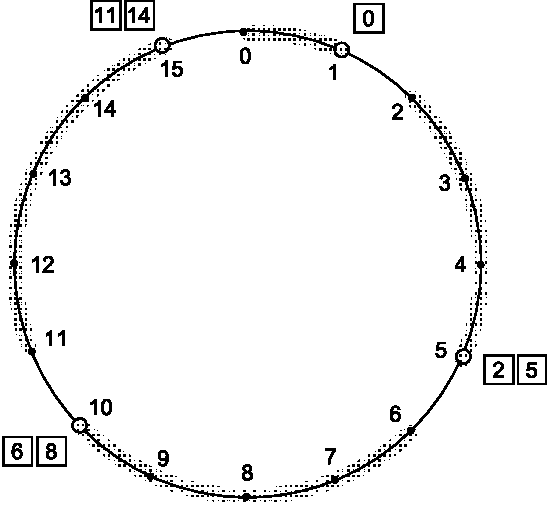
\includegraphics[width=0.4\textwidth]{pictures/pic0}\\
  \caption[Example of a $4$-bit Chord identifier circle]{Example of a $4$-bit Chord identifier circle.
  The responsibility ranges for each peer are accentuated in light gray}\label{fig:pic0}
\end{figure}
Es lassen sich auch mehrere Bilder nebeneinander platzieren wie z.B. in Abbildung
\ref{fig:multipic} zu sehen ist.
\begin{figure}[hpbt]
 \centering
  %%----start of first subfigure----
  \subfloat[FIFO size limited to 20 entries]{
   \label{fig:multipic:a} %% label for first subfigure
   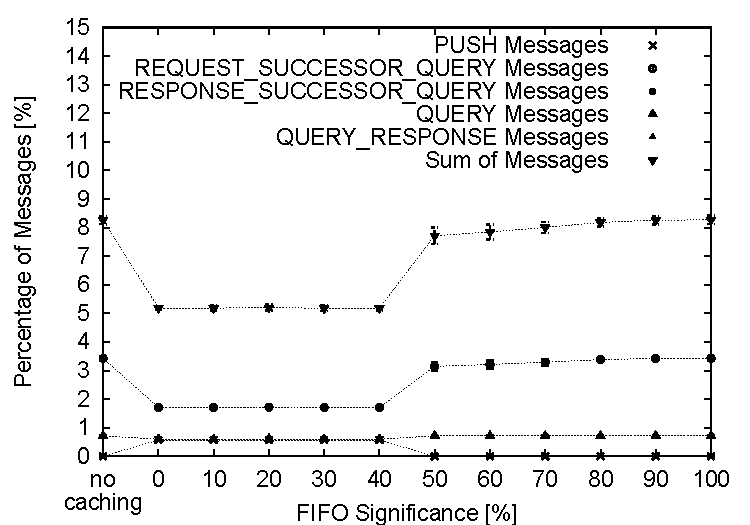
\includegraphics[width=0.48\linewidth]{pic1}}
  \hspace{0.01\textwidth}
  %%----start of second subfigure----
  \subfloat[FIFO size limited to 30 entries]{
   \label{fig:multipic:b} %% label for second subfigure
   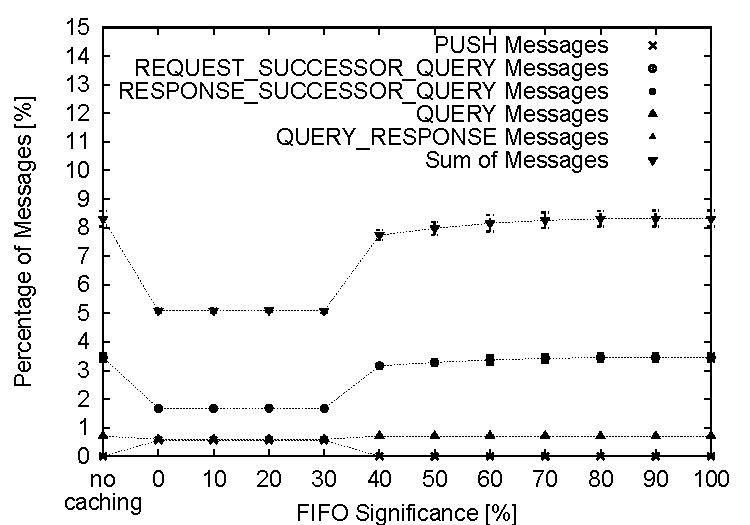
\includegraphics[width=0.48\linewidth]{pic2}}\\[0pt] % horizontal break
  %%----start of third subfigure----
  \subfloat[FIFO size limited to 40 entries]{
   \label{fig:multipic:c} %% label for third subfigure
   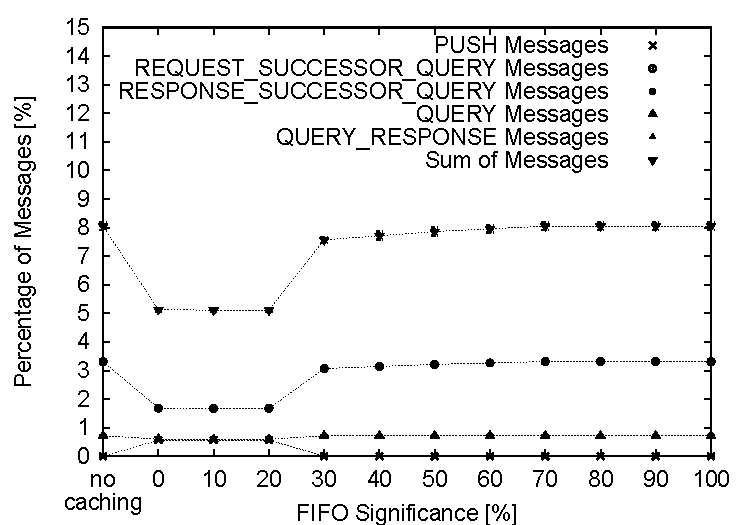
\includegraphics[width=0.48\linewidth]{pic3}}
  \hspace{0.01\textwidth}
  %%----start of fourth subfigure----
  \subfloat[FIFO size limited to 50 entries]{
   \label{fig:multipic:d} %% label for fourth subfigure
   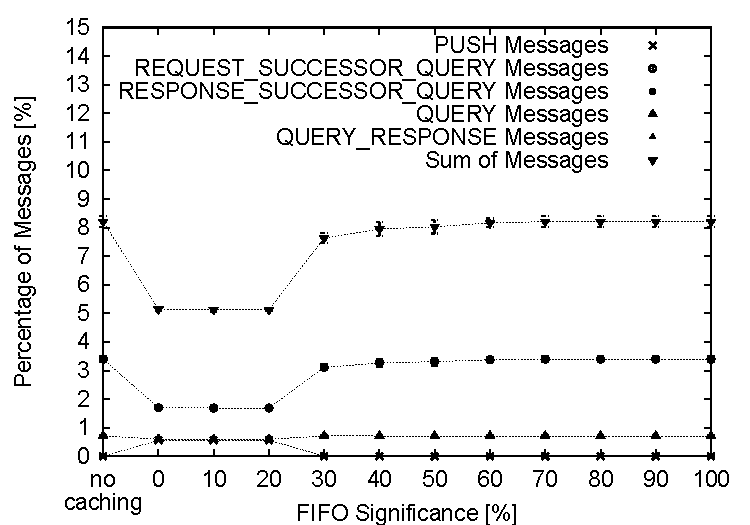
\includegraphics[width=0.48\linewidth]{pic4}}
 \caption[Observed message fractions and 95\% confidence intervals for Chord]{Observed message fractions and 95\% confidence intervals for Chord without the influence of churn. The FIFO capacity varies from 20 (\ref{fig:multipic:a}) -- 50 (\ref{fig:multipic:d}) entries (decadic steps).}
 \label{fig:multipic} %% label for entire figure
\end{figure}

\subsection{Programm Code}
Eine elegante M�glichkeit, Programmtext einzubinden, l�sst sich mit dem listings-Paket erreichen.
Das \verb|HelloWorld| Programm aus Listing \ref{lst:hw} hat in Zeile \ref{line:hw3} �brigens einen Programmierfehler.
\begin{lstlisting}[float=htp,caption=Hello World,label=lst:hw,language=Java, numbers=left, numberstyle=\tiny, stepnumber=2, numbersep=8pt, escapeinside={//@}{@//},backgroundcolor=\color{yellow},xleftmargin=3ex,xrightmargin=1ex]
public class HelloWorld {
    public static void main(String[] args) {
        Syste.out.println("Hello, World"); //@\label{line:hw3}@//
    }
}
\end{lstlisting}

\subsection{Fu�noten}
Wenn man auf Google \footnote{\url{http://www.google.com}} verweisen will, bietet sich statt einer gesonderten
Referenz auch einfach eine Fu�note an.
\subsection{Formeln}
Man kann mit \LaTeX\ sehr sch�n Formeln erzeugen:
$$L_{P}(k) = R^{orig}_{P}(k) + \sum_{i=0}^n 2*R^{i}_{P}(k)$$

    \chapter{Einleitung} \label{sec:introduction}
Eine der wohl herausstechendsten Fähigkeiten des Menschen ist es, durch das Sammeln von Erfahrungen immer neue Dinge zu lernen und auf diese Weise komplexe Zusammenhänge verstehen zu können. Es ist daher verständlich, dass uns die Idee der Entwicklung von künstlichen Intelligenzen, welche diese Fähigkeit ebenfalls besitzen, fasziniert. Bereits seit Ende des 20. Jahrhunderts haben sich viele Hollywood-Produktionen diese Faszination zu Nutzen gemacht. Wenn man erfolgreichen Filmreihen wie \glqq Matrix\grqq{} oder \glqq Terminator\grqq{} Glauben schenkt, so werden solche Maschinen früher oder später die Welt übernehmen. Stuart Russel, Professor an der University of California und Experte für künstliche Intelligenz, gibt hier zunächst Entwarnung: \glqq Hollywood's theory that spontaneously evil machine consciousness will drive armies of killer robots is just silly\grqq{} \cite{14_russell2016should}.

Die Angst vor Maschinen, die sich gegen uns wenden, ist trotzdem nicht ganz unbegründet. Russel sieht das Problem eher darin, dass eine künstliche Intelligenz überaus gut darin werden kann, eine andere Aufgabe zu lösen als die, die wir vorgesehen haben. Der Mathematiker Norbert Wiener erkennt bereits im Jahr 1960: \glqq If we use, to achieve our purposes, a mechanical agency with whose operation we cannot efficiently interfere..., we had better be quite sure that the purpose put into the machine is the purpose which we really desire.\grqq{} (\cite{14-2_wiener1960some}, zitiert nach \cite{14_russell2016should}). Es ist daher wichtig sicherzustellen, dass die künstliche Intelligenz tatsächlich das von uns gewünschte Ziel verfolgt.

Bei Reinforcement Learning wird die Aufgabe der lernenden Instanz über ein Signal der Umgebung formalisiert, dem \textit{Reward} \cite{06_sutton2018reinforcement}. Wir können der künstlichen Intelligenz nur indirekt über diese Belohnung vermitteln, was ihr Ziel ist. Der Reward spielt also eine sehr zentrale Rolle und ist eine mächtige Komponente im Bereich des Machine Learning, die mit Bedacht formuliert werden sollte.

Wir wollen in dieser Arbeit noch einen Schritt weiter denken und stellen uns die Frage, ob es möglich ist, auch komplexere Mechanismen ausschließlich im Reward zu codieren. Hierbei geht es um Strategien, die normalerweise im Trainings-Algorithmus implementiert werden und so eine zusätzliche Ebene darstellen die das, was der Agent eigentlich lernt, für uns verschleiert. Wir betrachten insbesondere die Erkundung des Environments.

Während der Drang Neues zu entdecken in der Natur des Menschen liegt, benötigt eine künstliche Intelligenz eine Strategie für das Erforschen des Umfelds, in dem sie sich befindet. Es existieren viele Strategien für die Erkundung der Umgebung des Agenten, doch eine der bekanntesten ist die $ \epsilon $-greedy-Strategie. Hierbei wählt der Agent meistens die beste ihm bekannte Aktion, probiert allerdings mit der Wahrscheinlichkeit $ \epsilon $ eine zufällige Aktion aus \cite{07_dabney2020temporallyextended, 06_sutton2018reinforcement}. Auf diese Weise wird erreicht, dass er bessere Lösungswege finden kann, die er davor noch nicht kannte.

\paragraph{Zielsetzung}
Wir experimentieren in dieser Arbeit mit dem Ansatz, eine Erkundungsstrategie allein durch die Modifikation des von der Umgebung zurückgegebenen Rewards abzubilden. Wir vergleichen den Trainingsverlauf und die Resultate dieses Ansatzes mit der $ \epsilon $-greedy-Strategie und einem Agenten ohne Erkundungsstrategie. Letzteres soll zeigen, ob unsere Methode an sich einen Vorteil bringt. Wir experimentieren auf zwei sehr unterschiedlichen Domänen, um zu sehen, ob es hier Unterschiede in der Performance unserer Strategie gibt. Ziel ist es zu prüfen, ob unser Ansatz eine Daseinsberechtigung hat und ob es lohnenswert ist, in dieser Richtung weiterzuforschen.

\paragraph{Aufbau der Arbeit}
In Kapitel \ref{sec:basics} erklären wir zunächst die Grundlagen von Q-Learning und Deep-Q-Learning. Außerdem beschreiben wir, wie wir diese in Python implementieren. In Kapitel \ref{sec:NavigationProblem} bauen wir zunächst eine eigene Domäne (Gebirgslandschaft), um maximale Kontrolle über das Environment zu haben. Im Anschluss führen wir auf dieser nach einigen einführenden Experimenten Versuche durch, bei denen wir eine Erkundungsstrategie nur durch die Modifikation des Rewards implementieren. Wir verwenden sowohl einen Q-Learning- als auch einen Deep-Q-Learning-Agenten und vergleichen unseren Ansatz mit der $ \epsilon $-greedy-Strategie und einem Agenten ohne Erkundungsstrategie. Unsere Methode zeigt hier ein ähnliches Lernverhalten wie $ \epsilon $-greedy, obwohl unser Agent immer greedy agiert. In Kapitel~\ref{sec:LunaLander} nutzen wir unsere Erkenntnisse aus Kapitel \ref{sec:NavigationProblem}, um unseren Ansatz auf der Domäne des Lunar Landers zu testen. Wie im Kapitel davor vergleichen wir unseren Ansatz mit der $ \epsilon $-greedy Strategie und einem Agenten ohne Erkundungsstrategie. Auch hierlässt sich die Tendenz erkennen, dass unsere Methode einen positiven Einfluss auf das Training hat. In Kapitel \ref{sec:relatedWork} betrachten wir verwandte Publikationen auf diesem Gebiet und vergleichen diese mit unserer Arbeit. Abschließend fassen wir in Kapitel \ref{sec:conclusion} unsere Ergebnisse zusammen, ziehen daraus ein Fazit und verweisen auf mögliche zukünftige Entwicklungen.
    \chapter{Gebirgslandschaft-Domäne}\label{sec:NavigationProblem}
Wir betrachten zunächst ein Landschaftsnavigationsproblem. Der Agent soll hier in einer zufällig generierten Landschaft unterschiedliche Aufgaben lösen.

%% Das Environment
\section{Das Environment}

Als Environment für die folgenden Experimente wollen wir eine Gebirgslandschaft erzeugen. Die Umgebung bildet hierbei ein Raster, worauf sich der Agent bewegen kann. Jeder Punkt auf dem Raster soll eine Höhe besitzen. Die Landschaft soll zufällig generiert werden können.

Die simpelste Lösung hierfür wäre wohl, ein zweidimensionales Array mit zufälligen Zahlen zu füllen. Auf diese Weise erhält man für jede Koordinate eine zufällige Höhe. Es ist allerdings für die Lesbarkeit des Problems essenziell, dass benachbarte Punkte einen Zusammenhang haben (zum Beispiel \glqq Bewegt sich der Agent gerade nach oben in die Richtung eines Gipfels oder nach unten in die Richtung eines Tals?\grqq). Dazu kommt, dass die Ergebnisse der Experimente intuitiv sichtbar sein sollen (zum Beispiel \glqq Hat der Agent einen Berg gefunden?\grqq). Deshalb wollen wir eine Landschaft erstellen, die organisch und natürlich aussieht.

% \subsection{Perlin Noise}
\paragraph{Perlin Noise}
Um dieses Ziel zu erreichen, verwenden wir \textit{Perlin Noise} \cite{parberry2015modeling}. Hierbei handelt es sich um eine Rauschfunktion, mit der sich sehr natürlich wirkende Texturen zufällig generieren lassen. Abbildung \ref{img:perlinNoise} zeigt eine simple Darstellung von zweidimensionalem Perlin Noise, bei der die generierten Werte mit Farbwerten von Schwarz bis Weiß abgebildet werden.
\begin{figure}[h!]
    \centering
    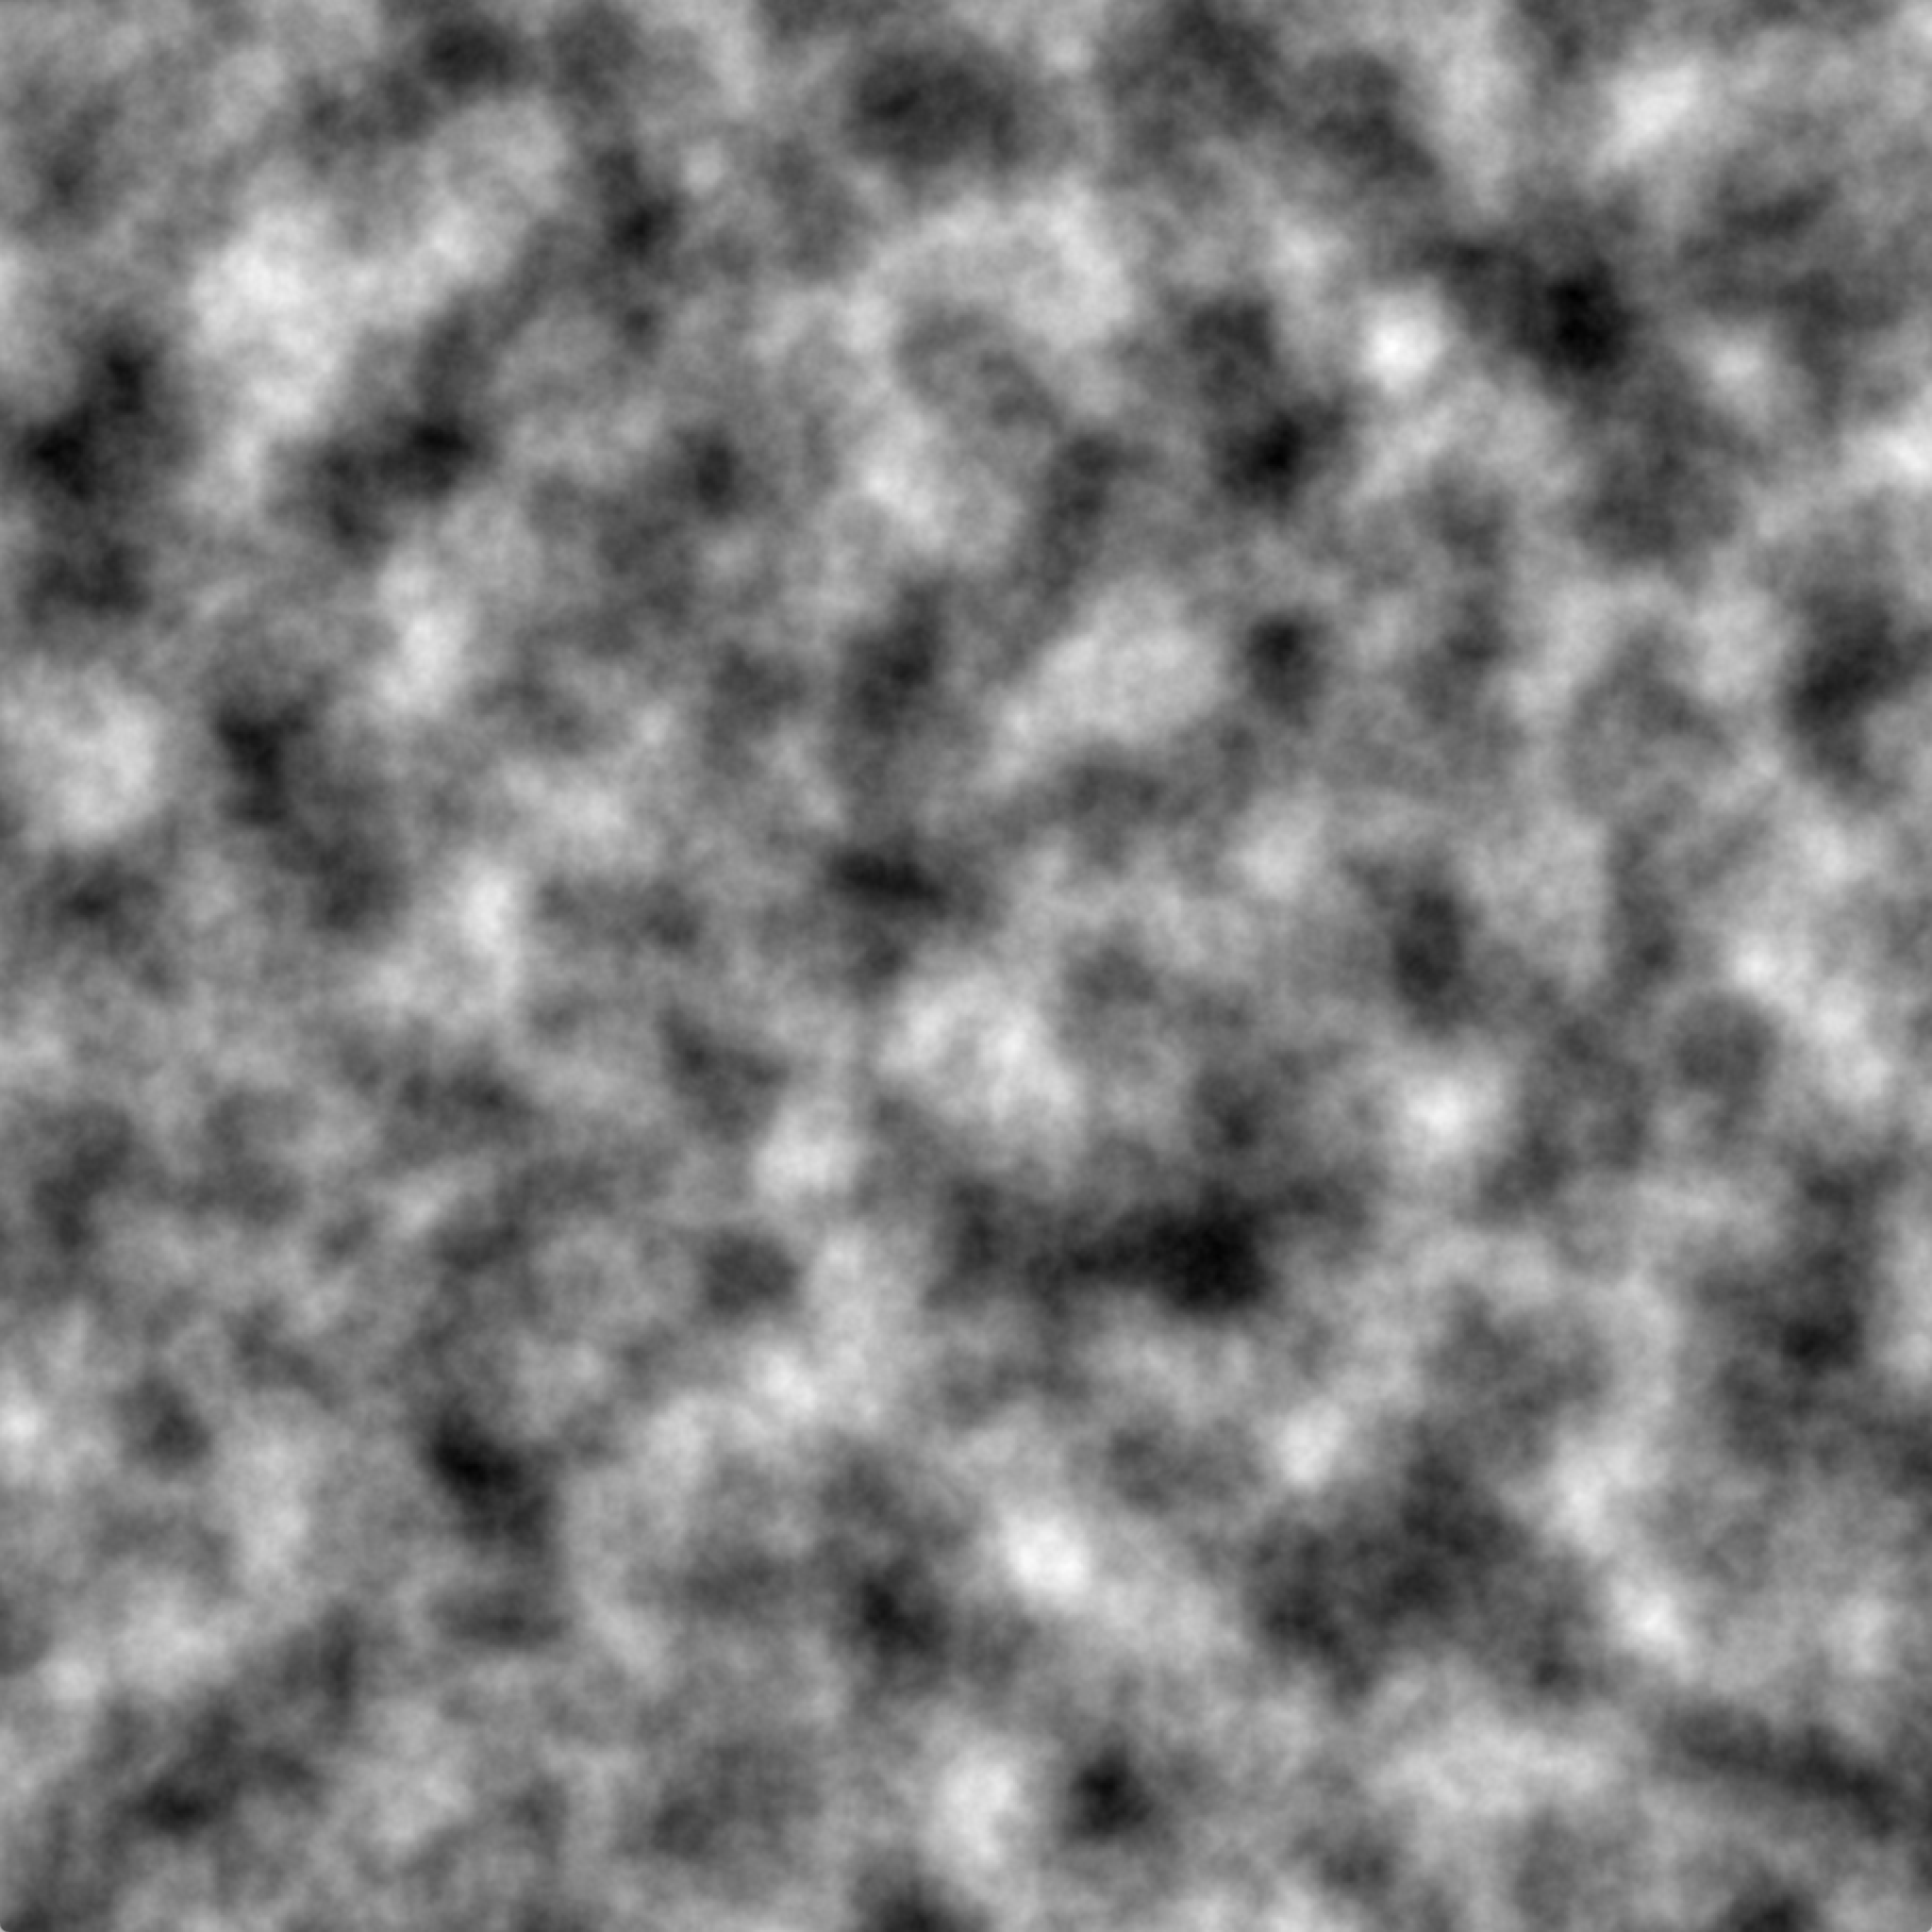
\includegraphics[width=0.5\textwidth, keepaspectratio=true]{perlin_noise.png}
    \caption{Visualisierung von zweidimensionalem Perlin Noise} \label{img:perlinNoise}
    \source{\url{https://miro.medium.com/max/2400/1*vs239SecVBaB4HvLsZ8O5Q.png}}
\end{figure}
Perlin Noise ist nach \cite{parberry2015modeling} ein fundamentaler Algorithmus in der prozeduralen Generierung von Terrain und somit offenbar sehr gut geeignet, um unsere Umgebung zu erstellen. Wir verwenden ihn um ein zweidimensionales Array mit zufälligen Werten zwischen -1 und 1 zu erzeugen, welche wir mit einer beliebigen Höhe multiplizieren können. Je nachdem, wie stark man in die Rauschfunktion \glqq hereinzoomt\grqq{}, erhält man unterschiedliche Verteilungen der Landschaft, wie man in Abbildung \ref{img:randomTerrain} erkennen kann.
\begin{figure}[h!]
    \centering
    \begin{subfigure}[b]{0.49\textwidth}
        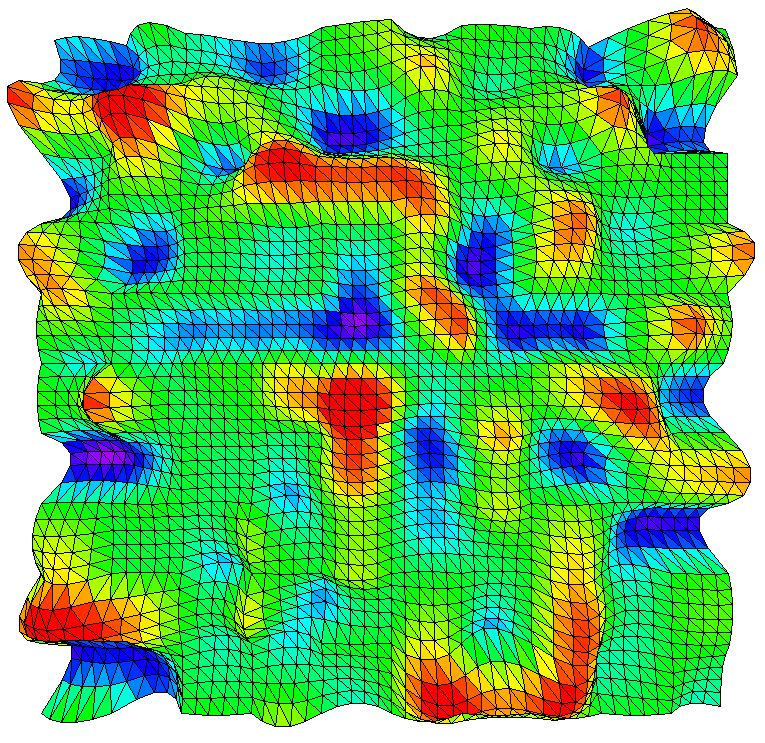
\includegraphics[width=\textwidth]{terrain_01.JPG}
        \caption{Landschaft mit niedriger Verteilung}
        \label{img:randomTerrainA}
    \end{subfigure}
    \begin{subfigure}[b]{0.49\textwidth}
        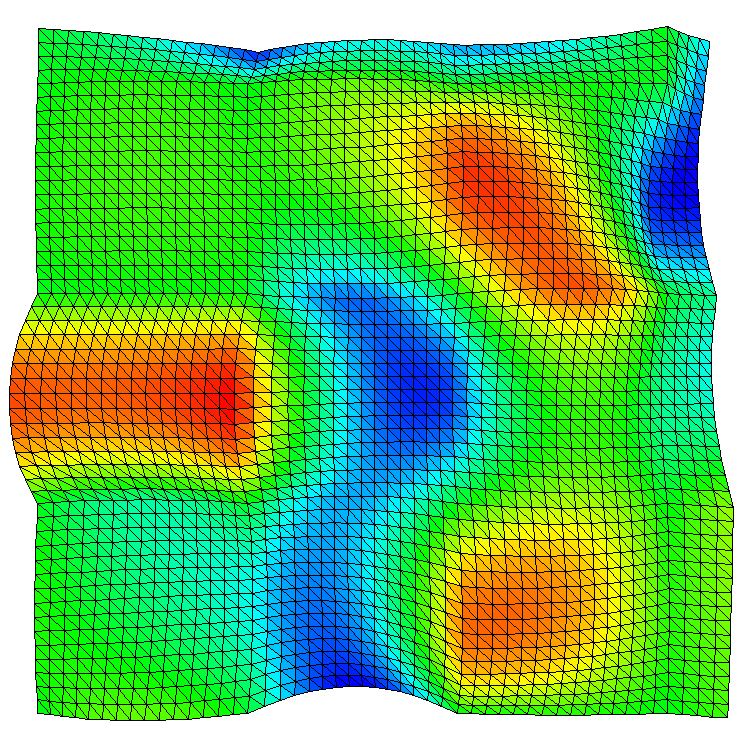
\includegraphics[width=\textwidth]{terrain_02.JPG}
        \caption{Landschaft mit hoher Verteilung}
        \label{img:randomTerrainB}
    \end{subfigure}
    \caption{Mittels Perlin Noise zufällig generierte Landschaften}
    \label{img:randomTerrain}
\end{figure}
Wir werden nicht näher auf die Details der Funktion eingehen, da dies nicht Kern dieser Arbeit ist. Für weitere Ausführungen diesbezüglich verweisen wir auf \cite{archer2011procedurally}.

Für die Visualisierung der Landschaft benutzen wir eine abgewandelte Form des Codes von \url{https://github.com/hnhaefliger/PyEngine3D} (Zugriff am 25.04.2021). Wir nutzen diese vergleichsweise simple 3D-Engine, damit wir alle Aspekte des Environments und dessen Visualisierung kontrollieren und für unseren Zweck anpassen können. So werden zum Beispiel zur besseren Differenzierung Berge und Täler -- zusätzlich zur perspektivischen Abhebung -- rot bzw. blau dargestellt.

Wir besitzen nun die Möglichkeit, eine zufällige Landschaft zu generieren und diese visuell darzustellen. Um bei allen Experimenten die gleichen Voraussetzungen zu gewährleisten, generieren wir mit der eben beschriebenen Methode zufällig ein Terrain, das allen folgenden Experimenten als Environment dient. Dieses ist in Abbildung \ref{img:terrainMain} dargestellt. Der höchste Punkt befindet sich bei dieser Landschaft auf dem Berg ganz oben in der Mitte.

\begin{figure}[h]
    \centering
    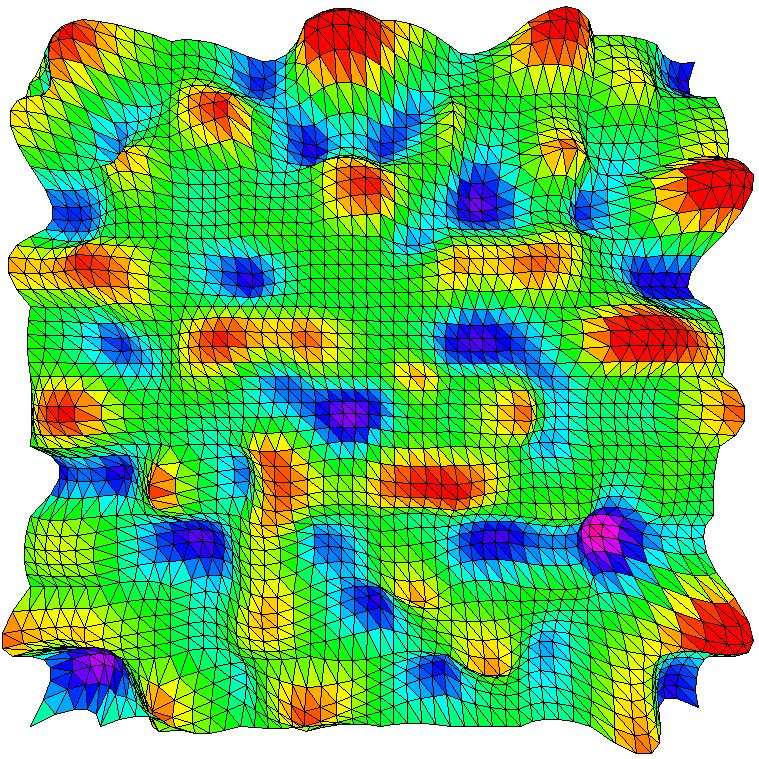
\includegraphics[width=0.5\textwidth, keepaspectratio=true]{terrain_main.JPG}
    \caption{Landschaft, auf der die Experimente durchgeführt werden} \label{img:terrainMain}
\end{figure}

%% Q-Learning Experiments
\section{Q-Learning-Experimente}

Um nun zu testen, ob die Landschaft für unsere Zwecke geeignet ist, werden wir einige Experimente durchführen. Wir wollen hierfür zunächst einen simplen Reinforcement-Learning-Agenten implementieren, welcher \textit{Q-Learning} verwendet.

\subsection{Das Prinzip von Q-Learning}
% \citeauthor{}

Dieses Kapitel stützt sich zu einem Großteil auf das Buch \textit{Reinforcement Learning: An Introduction, Second Edition} \cite{06_sutton2018reinforcement}. Falls nicht anders angegeben, wurden die Informationen hieraus entnommen.

\paragraph{Markov Decision Processes}
Alle folgenden Experimente zielen darauf ab, Probleminstanzen von \textit{Markov Decision Processes} -- oder kurz MDPs -- zu lösen. In MDPs gibt es eine handelnde Instanz, den \textit{Agenten}, welcher mit seinem Umfeld, der so genannten \textit{Umgebung} interagiert. Diese Interaktion erfolgt Sequenziell in Zeitschritten $ t = 0, 1, 2, 3, ... $. Der Agent erhält in jedem Zeitschritt $ t $ eine Repräsentation seiner Umgebung, den Zustand $ S_t $, und führt basierend darauf eine \textit{Aktion} $ A_t $ aus. Für diese erhält er von der Umgebung eine Belohnung $ R_{t + 1} $, sowie einen Folgezustand $ S_{t + 1} $.

\begin{figure}[H]
    \centering
    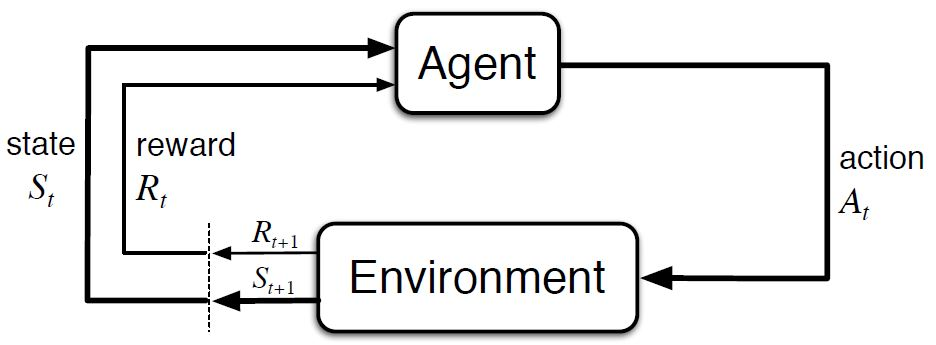
\includegraphics[width=0.5\textwidth, keepaspectratio=true]{mdp.JPG}
    \caption{Interaktion zwischen Umgebung und Agent in einem MDP} \label{img:mdp}
    \source{\cite{06_sutton2018reinforcement}}
\end{figure}

Ziel des Agenten ist es nun, seinen erwarteten Ertrag $ G_t $ zu maximieren. Im einfachsten Fall ist dieser die Summe aller Belohnungen:
\begin{align}
    G_t \doteq R_{t + 1} + R_{t + 2} + R_{t + 3} + ... + R_T \text{,} \label{eq:expected_reward}
\end{align}
wobei T Zeitschritt einer Episode ist. In vielen Fällen ist die Interaktion zwischen Agent und Umgebung allerdings nicht endlich. Somit ist in diesen Fällen $ T = \infty $ und der Ertrag, den der Agent maximieren soll, nach \ref{eq:expected_reward} unendlich. Wir führen deswegen das \textit{discounting} ein. Für $ G_t $ ergibt sich hiermit:
\begin{align}
    \begin{split}
        G_t & \doteq R_{t + 1} + \gamma R_{t + 2} + \gamma^2 R_{t + 3} + ...\\
        & = \sum_{k = 0}^{T} \gamma^k R_{t + k + 1} \text{,}
    \end{split} \label{eq:expected_discounted_reward}
\end{align}
wobei die \textit{discount rate} $ \gamma $ ein Wert zwischen $ 0 $ und $ 1 $ ist. Eine Belohnung $ k $ Zeitschritte in der Zukunft ist also nur $ \gamma^{k - 1} $--mal so viel wert wie eine Belohnung, welche im aktuellen Zeitschritt erhalten wurde.

\paragraph{Policies}
Der Agent folgt zu jedem Zeitpunkt einer Policy $ \pi $. Hierbei gibt $ \pi(a|s) $ die Wahrscheinlichkeit dafür an, dass der Agent zum Zeitschritt $ t $ die Aktion $ a \in A $ im Zustand $ s \in S $ ausführt, also dass die Aktion $ A_t = a $ wenn $ S_t = s $. Hierbei ist $ S $ die Menge aller Zustände und $ A $ die Menge aller Aktionen. $ \pi(a|s) $ ist also eine Wahrscheinlichkeitsverteilung über $ a \in A(s) $ für jedes $ s \in S $, wobei $ A(s) $ alle möglichen Aktionen im Zustand $ s $ beschreibt.

\paragraph{State-Value Functions}
Wir benötigen nun eine Möglichkeit einzuschätzen, wie gut ein Zustand $ s $ ist, wenn wir der Policy $ \pi $ folgen. Hierfür nutzen wir die \textit{state-value function} $ v_\pi $. Diese beschreibt die erwartete Belohnung eines Zustands $ s $ unter der Policy $ \pi $ zum Zeitschritt $ t $. Wir definieren $ v_\pi(s) $ als
\begin{align}
    \begin{split}
    v_\pi(s) & \doteq E_\pi \left[G_t | S_t = s \right]\\
    & = E_\pi \left[\sum_{k = 0}^{\infty} \gamma^k R_{t + k + 1} | S_t = s \right],
    \end{split}
\end{align}
wobei $ E_\pi $ der Erwartungswert des Ertrags $ G_t $ nach \ref{eq:expected_discounted_reward} ist, wenn der Agent sich im Zustand $ S_t = s $ befindet und der Policy $ \pi $ folgt.

\paragraph{Action-Value Functions}
Ähnlich hierzu gibt die \textit{action-value function} $ q_\pi $ an, wie profitabel es für den Agenten ist, in einem gegebenen Zustand eine gewisse Aktion auszuführen, wenn der Agent der Policy $ \pi $ folgt.

Der Wert einer Aktion $ a $ im Zustand $ s $ unter der Policy $ \pi $ ist also die erwartete Belohnung, wenn man im Zustand $ s $ zum Zeitschritt $ t $ die Aktion $ a $ ausführt. Wir definieren $ q_\pi(s, a) $ als
\begin{align}
    \begin{split}
    q_\pi(s,a) & \doteq E_\pi \left[G_t | S_t = s, A_t = a \right]\\
    & = E_\pi \left[\sum_{k = 0}^{\infty} \gamma^k R_{t + k + 1} | S_t = s, A_t = a \right].
    \end{split}
\end{align}
Die action-value function wird auch als Q-function bezeichnet, welche als Ergebnis für ein state-action Paar die Q-value liefert. Für die folgenden Implementierungen ist diese von großer Wichtigkeit.

\paragraph{Optimale Policies und Optimale Value Functions}
Das Ziel des Agenten ist, die optimale Policy $ \pi $ für ein Markov Decision Problem zu finden. Ist dieses Ziel erreicht so lässt sich sagen, dass die Reinforcement Learning Aufgabe erfüllt ist. Optimal ist hierbei die Policy, welche nach Aufsummieren der Belohnungen über alle Schritte einer Episode die beste gesamte Belohnung liefert. Eine Policy $ \pi $ ist also besser als Policy $ \pi' $, wenn die erwartete Belohnung von $ \pi $ für \textbf{alle} Zustände $ s \in S $ größer ist als die von $ \pi' $. \cite{06_sutton2018reinforcement} verwendet die Formulierung
\begin{align}
    \pi \geq \pi' \text{ if and only if } v_\pi(s) \geq v_{\pi'}(s) \text{ for all } s \in S.
\end{align}

Es gibt immer eine Policy, die besser als oder gleichwertig mit allen anderen Policies ist. Diese wird beziehungsweise werden als $ \pi_* $ bezeichnet. Die besten Policies besitzen die gleich state-value function, welche die \textit{optimale state-value function} $ v_* $ genannt wird und definiert wird als
\begin{align}
    v_*(s) \doteq \max_\pi v_\pi(s)
\end{align}
für alle $ s \in S $.

Optimale Policies teilen sich ebenfalls die gleiche \textit{optimale action-value function} $ q_* $, welche definiert ist als
\begin{align}
    q_*(s, a) \doteq \max_\pi q_\pi(s, a)
\end{align}
für alle $ s \in S $ und $ a \in A $. $ q_* $ liefert also für jedes state-action Paar den größtmöglichen erwarteten Ertrag, den irgendeine Policy erreichen kann.

\paragraph{Bellman Optimality Equation}
Die optimale action-value function $ q_* $ muss die folgende Gleichung erfüllen:
\begin{align}
    q_*(s, a) = E \left[R_{t + 1} + \gamma \max_{a'} q_*(s', a') \right] \label{eq:bellman}
\end{align}
Diese Gleichung wird \textit{Bellman optimality equation} für $ q_* $ genannt und besagt, dass der beste erwartete Ertrag für jedes state-action Paar $ (s, a) $ zum Zeitpunkt $ t $ der Summe aus der direkten Belohnung $ R_{t + 1} $ der Aktion $ a $ und dem \textbf{maximalen} erwarteten Ertrag, der von einem der nächsten state-action Paare $ (s', a') $ erreicht werden kann entsprechen muss. Hierbei ist $ s' $ der Folgezustand $ S_{t + 1} $ und $ a' $ die Aktion $ A_{t + 1} \in A(s') $, welche den meisten Ertrag bringt.

Das folgende Kapitel beschreibt, wie die Bellman equation verwendet wird, um $ q_* $ zu finden, was uns wiederum die optimale Policy liefern soll. 

\subsection{Der Ablauf von Q-Learning} \label{sec:q_learning_process}
Das Ziel von Q-Learning ist, die optimale Policy zu finden, indem der Agent die optimalen Q-values für jedes state-action Paar erlernt.

Der Q-Learning Algorithmus benutzt die Bellman equation als Update-Regel, um nach und nach die Q-values für jedes state-action Paar anzunähern. Dieses Verfahren nennt man \textit{value iteration}.

Bei überschaubaren Umgebungen ist es möglich, die Werte für jedes state-action Paar in einer Tabelle, der so genannten \textit{Q-table} zu speichern. Zu Beginn weiß der Agent nichts über eine Umgebung. Die Q-table ist dementsprechend leer beziehungsweise ist der Wert jedes state-action Paares 0. Der Agent operiert nun eine vorbestimmte Anzahl von \textit{Episoden} in der Umgebung und produziert im Laufe der Zeit neue Q-values, mit denen die Q-table aktualisiert wird.

Zu Beginn jedes Schritts -- auch \textit{step} genannt -- wählt der Agent eine Aktion für den aktuellen Zustand aus. Intuitiv macht es Sinn, die beste bisher bekannte Aktion zu wählen, um die Belohnung zu maximieren. Dieses Vorgehen ist allerdings nicht zielführend, da der Agent ja am Anfang nichts über seine Umgebung weiß. Er benötigt also für die Wahl seiner Aktionen eine bessere Strategie. Auf dieses Problem gehen wir in Kapitel \ref{sec:exploration_exploitation} näher ein.

Nehmen wir an, der Agent hat im Zustand $ s $ zum Zeitschritt $ t $ eine Aktion $ a $ ausgewählt. Nach der Bellman equation \ref{eq:bellman} ist dann die Q-value $ q(s, a) $ (der Übersicht in Gleichung \ref{eq:updateQValue} wegen wird die Policy $ \pi $ hier weggelassen) die für die Aktion erhaltene Belohnung $ R_{t + 1} $ plus der maximale erwartete Ertrag eines folgenden state-action Paares, also
\begin{align}
    q(s, a) = R_{t + 1} + \gamma \max_{a'} q(s', a'). \label{eq:bellmanClean}
\end{align}
Dies berücksichtigt allerdings nicht, dass der Agent in einem früheren Zeitschritt oder in einer anderen Episode vielleicht bereits einen Wert $ q(s, a) $ für dieses state-action Paar berechnet und in der Q-table gespeichert hat. So wird bei jeder Berechnung eventuell ein alter Wert überschrieben und vergangene Erkenntnisse haben keinen Einfluss auf die aktuelle Berechnung.

Ein besserer Ansatz ist die Verwendung einer \textit{learning rate}. Die learning rate ist ein Wert zwischen 0 und 1, der festlegt, wie schnell der Agent vergangene Q-values aus der Q-table verwirft. Anders gesagt legt sie fest, wie viel Information aus vorherigen Berechnungen bei einem Update einer Q-value erhalten bleibt. Wir verwenden für die learning rate das Symbol $ \alpha $.

Für die Berechnung der neuen Q-value für das state-action Paar $ (s, a) $ zum Zeitpunkt $ t $ ergibt sich dann
\begin{align}
    q_\text{neu}(s, a) = (1 - \alpha) q(s, a) + \alpha \left(R_{t + 1} + \gamma \max_{a'} q(s', a') \right). \label{eq:updateQValue}
\end{align}
Bei einer learning rate von $ \alpha = 0.6 $ bleiben so $ 40\% $ des alten Wertes erhalten, während der neu erlernte Wert mit $ 60\% $ gewichtet wird.

\subsection{Exploration vs Exploitation} \label{sec:exploration_exploitation}
In Kapitel \ref{sec:q_learning_process} sind wir auf die Notwendigkeit einer Strategie, mit der der Agent seine nächste Aktion auswählt, gestoßen. Wie dort bereits erwähnt ist eine sehr simple Methode die Auswahl der Aktion mit der größten erwarteten Belohnung. Eine solche Aktion wird \textit{greedy} Aktion genannt. Gibt es mehrere greedy Aktionen mit demselben erwarteten Ertrag, so wird eine davon zum Beispiel per Zufall ausgewählt.

Diese Strategie klingt auf den ersten Blick sinnvoll, ist aber nicht so zielführend wie es scheint. Der Agent versäumt es andere Aktionen auszuprobieren, die eine bessere Belohnung liefern könnten. Er nutzt nur die ihm bekannten aus (engl. \textit{exploitation}). Besser wäre es, wenn er ebenfalls Zeit in die Erkundung (engl. \textit{exploration} der Umgebung stecken würde.

Dies kann realisiert werden, indem der Agent die meiste Zeit \glqq gierig\grqq{} (engl. greedy) agiert und die Aktion mit dem besten geschätzten Ertrag wählt, mit einer Wahrscheinlichkeit von $ \epsilon $ allerdings ab und zu zufällig eine von allen verfügbaren Aktionen auswählt. $ \epsilon $ ist hierbei ein Wert zwischen 0 und 1, der entweder statisch oder dynamisch definiert wird. Auf diese Weise wird erreicht, dass der Agent auch Aktionen ausprobieren kann, welche er zuvor noch nicht gesehen hat. Methoden, welche nach diesem Schema agieren, werden \textit{$ \epsilon $-greedy} Methoden genannt und zählen nach \cite{07_dabney2020temporallyextended} auch heute noch bei der Erkundung der Umgebung zu den am meisten benutzten.
% Ref zu Beispiel

\subsection{Implementierung in Python} \label{sec:qLearningImplementation}
Mit diesem Wissen werden wir nun einen Q-Learning Algorithmus in Python implementieren.

\paragraph{Hyperparameter} \label{sec:qLearningHyperparameter}
In den vorherigen Kapiteln haben wir einige Variablen eingeführt, von denen uns manche als so genannte \textit{Hyperparameter} dienen werden \cite{08_ravichandiran2018hands}. Diese steuern das Verhalten des Agenten und sollten für den optimalen Lernerfolg angepasst werden. Wir verwenden hierfür eine selbst definierte Datenklasse, um alle Hyperparameter an zentraler Stelle verwalten zu können:
\begin{minted}{python}
@dataclass
class Parameters:
    num_episodes: int
    max_steps_per_episode: int

    learning_rate: float
    discount_rate: float

    start_exploration_rate: float
    max_exploration_rate: float
    min_exploration_rate: float
    exploration_decay_rate: float

    rewards_all_episodes: list
    max_rewards_all_episodes: list
\end{minted}
\mintinline{python}{num_episodes} gibt die Anzahl der Episoden an, die der Agent trainieren soll, \linebreak\mintinline{python}{max_steps_per_episode} die Schritte pro Episode. \mintinline{python}{learning_rate} und \mintinline{python}{discount_rate} sind selbsterklärend. Die folgenden vier Werte beziehen sich auf die $ \epsilon $-greedy Strategie. Wir wollen die Möglichkeit haben, unser $ \epsilon $ dynamisch anzupassen. Hierfür initialisieren wir die \mintinline{python}{start_exploration_rate} als unser Anfangs-$ \epsilon $, die \mintinline{python}{max_exploration_rate} als Absicherung und eventuelle Variable für die Zukunft (ist normalerweise identisch mit der \mintinline{python}{start_exploration_rate}), die \mintinline{python}{min_exploration_rate} als minimales $ \epsilon $ und die \mintinline{python}{exploration_decay_rate} als Größe die festlegt, wie schnell $ \epsilon $ schrumpfen soll. Hierzu in den folgenden Kapiteln (TODO) mehr. In den beiden Variablen \mintinline{python}{rewards_all_episodes} und \mintinline{python}{max_rewards_all_episodes} werden die Belohnungen des Trainings abgelegt.

\paragraph{Die \mintinline{python}{train()}-Methode}
(TODO Code reference). Die \mintinline{python}{train()}-Methode ist das Herzstück des Algorithmus. Sie besitzt die folgenden Parameter:
\begin{minted}{python}
def train(self, width: int, length: int, params: Parameters,
            environment, visualize=False, plot=False, plot_interval=1,
            plot_moving_avg_period=100):
\end{minted}
\mintinline{python}{width} und \mintinline{python}{length} beschreiben die Breite und die Länge des Rasters aus \ref{img:terrainMain}, sprich die Größe der Landschaft. Mit diesen Daten wird die Größe der Q-table bestimmt. Mit den \mintinline{python}{params} übergeben wir der Funktion die Hyperparameter. Das \mintinline{python}{environment} ist die Umgebung des Agenten (TODO genauer). Die restlichen Parameter sind optional und beziehen sich auf die Visualisierung der Ergebnisse während des Trainings.
% \mintinline{python}{visualize} legt fest, ob der Agent in Echtzeit auf der Landschaft aus \ref{img:terrainMain} angezeigt wird. \mintinline{python}{plot} bestimmt, ob die erhaltenen Belohnungen in einem Graphen ausgegeben werden sollen und falls ja geschieht das alle \mintinline{python}{plot_interval} Episoden. Der Graph zeigt dann außerdem einen Durchschnitt der letzten \mintinline{python}{plot_moving_avg_period} Episoden.

Wir verwenden für die Implementierung der Q-table \textit{NumPy}, die primäre Bibliothek für die Array-Programmierung in Python \cite{harris2020array}. Wir erzeugen ein zweidimensionales NumPy-Array, das für jeden Zustand unserer Umgebung eine Zeile und für jede Aktion (in unserem Fall die Bewegung nach oben, rechts, unten und links) eine Spalte enthält. Alle Elemente werden zunächst mit 0 initialisiert. Außerdem setzen wir unser $ \epsilon $ auf die in den Hyperparametern festgelegte \mintinline{python}{start_exploration_rate}. Wir erstellen außerdem einen Buffer, welcher die Tupel aus Zustand, Aktion, Belohnung und Folgezustand enthält. Dieser wird am Ende jeder Episode gemischt und dann abgearbeitet. Dieses Verfahren löst nach TODO starke Pfadabhängigkeiten auf. In Kapitel \ref{sec:deepQPrinciple} gehen wir hierauf näher ein.
\begin{minted}{python}
    q_table = np.zeros((width * length, 4))
    exploration_rate = params.start_exploration_rate
    buffer = []
\end{minted}

Zu Beginn jeder Episode setzen wir den Zustand auf den Startzustand der Umgebung und erzeugen die beiden Variablen, die die Belohnungen der Episode speichern:
\begin{minted}{python}
    for episode in range(params.num_episodes):
        state = environment.reset_agent()
        rewards_current_episode = 0
        max_reward_current_episode = 0
\end{minted}

In jedem Zeitschritt wenden wir für die Wahl der Aktion unsere $ \epsilon $-greedy Strategie an. Hierfür erzeugen wir eine zufällige Zahl zwischen 0 und 1. Falls diese größer ist als unser aktuelles $ \epsilon $, wählt der Agent die beste bekannte Aktion, ansonsten wird aus den möglichen Aktionen zufällig eine ausgewählt. Die Umgebung liefert uns infolgedessen den Folgezustand und die erhaltene Belohnung. Anschließend speichern wir das Tupel im Buffer, aktualisieren den Zustand, speichern die Belohnungen und zeigen ggf. die Position des Agenten an:
\begin{minted}{python}
        for step in range(params.max_steps_per_episode):
            exploration_rate_threshold = random.uniform(0, 1)
            if exploration_rate_threshold > exploration_rate:
                action = np.argmax(q_table[state, :])
            else:
                action = random.choice(
                    environment.get_agent_possible_actions()
                )
            new_state, reward, _ = environment.agent_perform_action(action)
            sars = (state, action, reward, new_state)
            buffer.append(sars)

            q_table[state, action] = (1 - params.learning_rate) *\
            q_table[state, action] + params.learning_rate * (reward +\
            params.discount_rate * np.max(q_table[new_state, :]))

            state = new_state
            rewards_current_episode += reward
            if max_reward_current_episode < reward:
                max_reward_current_episode = reward

            if visualize:
                environment.redraw_agent()
                time.sleep(0.04)
\end{minted}

Am Ende jeder Episode aktualisieren wir die entsprechenden Einträge in der Q-table mit den Daten aus dem Buffer. Hierfür wird die Gleichung für die Berechnung der Q-value \ref{eq:updateQValue} angewendet:
\begin{minted}{python}
        random.shuffle(buffer)
        while len(buffer) > 0:
            (state, action, reward, new_state) = buffer.pop(0)
            q_table[state, action] = (1 - params.learning_rate) *\
            q_table[state, action] + params.learning_rate * (reward +\
            params.discount_rate * np.max(q_table[new_state, :]))
\end{minted}

Außerdem wird das neue $ \epsilon $ berechnet. Wir verwenden hierfür eine exponentielle Funktion, damit $ \epsilon $ am Anfang start abfällt und gegen Ende langsamer. Zuletzt werden die Belohnungen in den Params gespeichert und ggf. als Graph angezeigt.
\begin{minted}{python}
        exploration_rate = params.min_exploration_rate +\
        (params.max_exploration_rate - params.min_exploration_rate) *\
        np.exp(-params.exploration_decay_rate * episode)

        params.rewards_all_episodes.append(rewards_current_episode)
        params.max_rewards_all_episodes.append(max_reward_current_episode)
        if plot and episode % plot_interval == 0:
            plot_progress(params.rewards_all_episodes, exploration_rate, plot_moving_avg_period)

    return q_table, params
\end{minted}

\smallspace

\subsection{Experimente} \label{sec:qLearningExperiments}
Nachdem der Agent implementiert ist, wollen wir diesen in unserer Umgebung testen. Wir verwenden die zuvor beschriebene Landschaft \ref{img:terrainMain}. Ziel ist es, dass der Agent den höchsten Gipfel erreicht. Zu diesem Zweck liefert die Umgebung als Belohnung die Differenz der Höhe des alten und neuen Zustands. Wenn sich der Agent also von einem Feld mit der Höhe $ 2.3 $ in ein Feld mit der Höhe $ 1.8 $ bewegt erhält er als Belohnung $ -0.5 $.

\paragraph{Einzelnes Experiment}
Nach einigem Ausprobieren haben sich die folgenden Hyperparameter als solche erwiesen, die gute Ergebnisse erzielen:
\begin{minted}{python}
params = Parameters(
            num_episodes=10000,
            max_steps_per_episode=300,
            learning_rate=0.6,
            discount_rate=0.99,
            start_exploration_rate=1,
            max_exploration_rate=1,
            min_exploration_rate=0.01,
            exploration_decay_rate=0.00015,
            # ... Rest wird erst während des Trainigs belegt
        )
\end{minted}

Wir stellen die Ergebnisse in einem Graph da. Nach einem Trainingdurchlauf erhält man die in \ref{img:graphQBest} dargestellte Ausgabe. Die x-Achse stellt die aktuelle Episode dar, während die y-Achse die erhaltene Belohnung, bzw. für die türkise Linie das $ \epsilon $ angibt. Die blaue Linie, welche aufgrund der großen Menge an unterschiedlichen Werten kaum mehr als solche zu erkennen ist, zeigt die Summe der Belohnungen aus allen Zeitschritten für jede Episode an. Die orange Linie ist der Durchschnitt der letzten 100 Gesamtbelohnungen pro Episode. Dieser Wert wird auch als \textit{moving average} bezeichnet. Die Werte von Episode 0 bis 99 sind hier mit 0 belegt. Die türkise Linie zeigt das $ \epsilon $ zu jeder Episode. Die Beschriftung hierfür befindet sich auf der rechten Seite des Graphen.

Es lässt sich an der orangen Linie gut erkennen, wie der Agent mit der Zeit immer bessere Belohnungen erhält.

Lässt man den Agenten nun die im Training erzeugt Q-table verwenden, um die beste Aktion für jeden Zeitschritt auszuwählen, so folgt er dem in \ref{img:pathQBest} sichtbaren Pfad. Er findet also den höchsten Berg in der gegebenen Landschaft, obwohl dieser weit entfernt vom Startpunkt in der Mitte und hinter einem Graben liegt.

\begin{figure}[H]
    \centering
    \begin{subfigure}[b]{0.49\textwidth}
        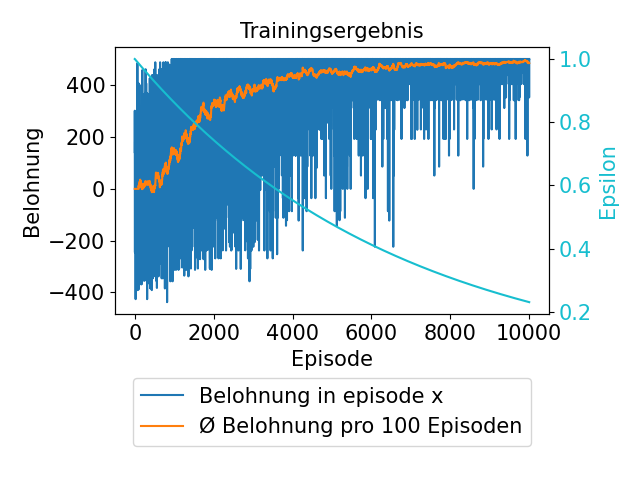
\includegraphics[width=\textwidth]{q_learning/figure_best.png}
        \caption{x-Achse zeigt die Episode, y-Achse zeigt die Belohnung. Eingezeichnet sind exakte Belohnung (blau), deren moving average (orange) und der Wert von $ \epsilon $ (türkis, Achse rechts) pro Episode.}
        \label{img:graphQBest}
    \end{subfigure}
    \begin{subfigure}[b]{0.49\textwidth}
        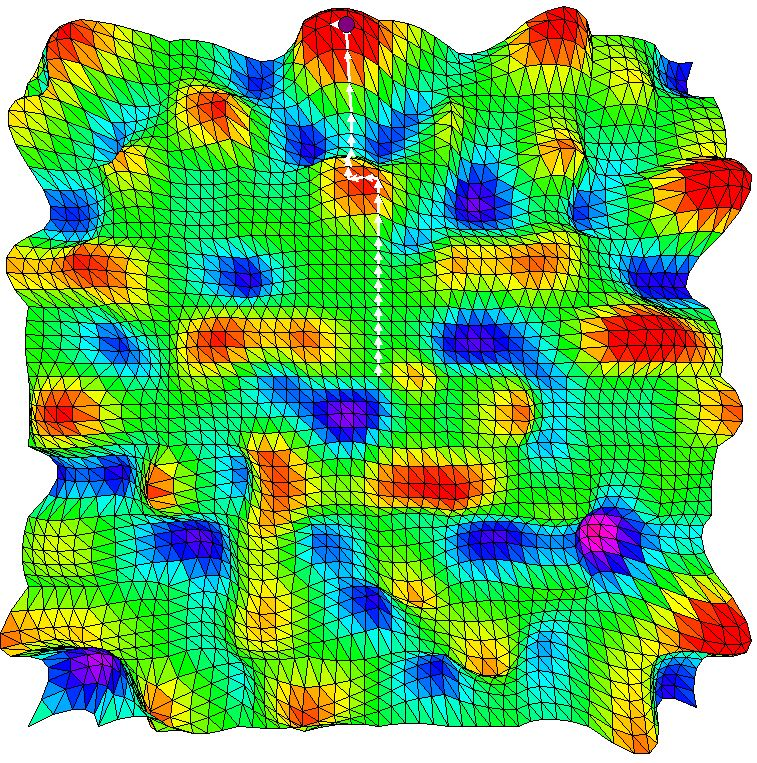
\includegraphics[width=\textwidth]{q_learning/terrain_path_best_white_3.JPG}
        \caption{Bester Pfad des Agenten nach dem Training}
        \label{img:pathQBest}
    \end{subfigure}
    \caption{Trainingsergebnisse des ersten Experiments}
\end{figure}

Eine weiter interessanter Wert ist die Anzahl der mit 0 belegten Einträge in der Q-table. Diese besitzen entweder zufällig den errechneten Q-value 0 oder wurden vom Agenten nicht berechnet. Da die meisten Einträge im 14-Stelligen Nachkommabereich liegen, ist ersteres relativ unwahrscheinlich und so lässt sich sagen, dass die Summe der mit 0 belegten Einträge ungefähr der Summe der nicht erkundeten Zustände entspricht. In Fall des aktuellen Experiments sind 850 der 10000 Einträge mit 0 belegt. Der Agent hat also ungefähr $ 91.5\% $ der Umgebung erkundet.

Dies ist nur ein einzelnes Experiment und hat natürlich keine statistische Aussagekraft. Es diente lediglich der Demonstration und der Erklärung der Visualisierung. Wir werden im Folgenden testen, welche Auswirkung die Verwendung der $ \epsilon $-greedy Strategie auf den Lernprozess hat.

\paragraph{Vergleich des Trainings mit und ohne $ \epsilon $-greedy Strategie}
Um eine aussagenkräftigere Datengrundlage zu erhalten, werden wir die folgenden Experimente jeweils 20 mal wiederholen. Diese Zahl hat sich als ein gutes Mittelmaß zwischen einer ausreichenden Menge an Daten für die Statistik und der Berechenbarkeit in zumutbarer Zeit erwiesen.

Die erste Experimentreihe erfolgt mit den gleichen Parametern wie im vorherigen Experiment. Für die zweite Experimentreihe setzen wir lediglich $ \epsilon $ auf 0. Das kommt dem Weglassen der $ \epsilon $-greedy Strategie gleich und bedeutet, dass der Agent in jedem Fall greedy agiert und die beste Aktion wählt. Dies soll die Notwendigkeit von $ \epsilon $ für ein besseres Trainingsergebnis zeigen.
\begin{figure}[H]
    \centering
    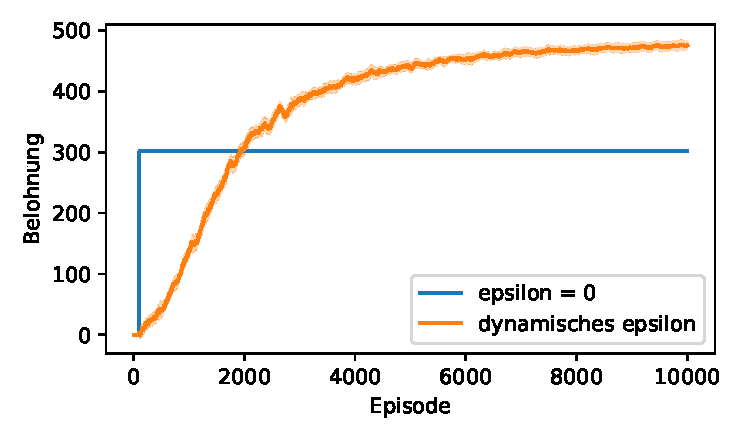
\includegraphics{q_learning/figure_epsilon_compare.pdf}
    \caption{Vergleich der Trainingsverläufe mit und ohne $ \epsilon $-greedy Strategie nach jeweils 20 Wiederholungen. Der Graph zeigt den moving average und dessen Standardabweichung pro Episode.} \label{img:graphQEpsComp}
\end{figure}
Die Achsen von Graph \ref{img:graphQEpsComp} sind bis auf das Fehlen der $ \epsilon $-Achse identisch mit dem aus \ref{img:graphQBest}. Die beiden Linien zeigen jeweils den Durchschnitt der moving average Werte aller 20 Experimentiterationen. Der leicht transparente Bereich um die Linien herum ist die Standartabweichung in der jeweiligen Episode.
Es lässt sich hier sehr deutlich erkennen, dass der Agent ohne eine Erkundungsstrategie wie $ \epsilon $-greedy (blaue Linie) zu Beginn einen relativ lukrativen Pfad findet, diesen aber dann auch nicht mehr verlässt, um andere Pfade zu erkunden und so immer die gleiche Belohnung bekommt. Er wird schließlich vom $ \epsilon $-greedy Agenten (orange Linie) überholt, da dieser seine Umgebung erkundet. Dieser erhält am Ende des Trainings wesentlich höhere Belohnungen.

Betrachten wir den Durchschnitt der Anzahl der mit 0 belegten Einträge der Q-tables beider Experimentreihen lässt sich abschätzen, dass der $ \epsilon $-greedy Agent im Schnitt $ 89.9\% $ der Umgebung erkundet hat, während es beim Agent ohne Erkundungsstrategie gerade einmal $ 1.1\% $ sind.

Dies zeigt, dass eine Erkundungsstrategie für den Erfolg des Agenten sehr wichtig ist.

\paragraph{Erkundungsstrategie codiert im Reward}
Für das nächste Experiment lassen wir der Agenten ebenfalls in jedem Zeitschritt greedy agieren. Diesmal erreichen wir dies, indem wir unabhängig vom aktuellen $ \epsilon $ immer die beste Aktion auswählen. Der Agent soll allein durch die Veränderung der Belohnung dazu gebracht werden, seine Umgebung besser zu erkunden und trotzdem einen möglichst hohen Punkt zu finden.

Wir modifizieren hierfür die nach jeder Aktion von der Umgebung erhaltene Belohnung wiefolgt:
\begin{minted}{python}
new_state, actual_reward, _ = environment.agent_perform_action(action)

reward = ((1 - exploration_rate) * actual_reward) - exploration_rate

sars = (state, action, reward, new_state)
buffer.append(sars)
\end{minted}
Die \mintinline{python}{exploration_rate} verhält sich hierbei genau so wie beim Experiment davor. Diese Formel soll bewirken, dass der Agent zu Beginn bei einer hohen \mintinline{python}{exploration_rate} alle besuchten Felder mit einem negativen Wert belegt, sodass er beim nächsten mal andere Felder besucht und so seine Umgebung erkundet. Nach und nach wird diese Belegung dann immer mehr mit den mittels korrekter Belohnungen ermittelten Q-values ersetzt, wodurch sich der Agent auf die besten Zustände einpendeln soll. Wir setzen die learning rate auf 1, damit der Agent nicht an den zu Beginn verfälschten Belohnungen festhält. Nach 50000 Episoden erhält man folgendes Ergebnis:
\begin{figure}[H]
    \centering
    \begin{subfigure}[b]{0.49\textwidth}
        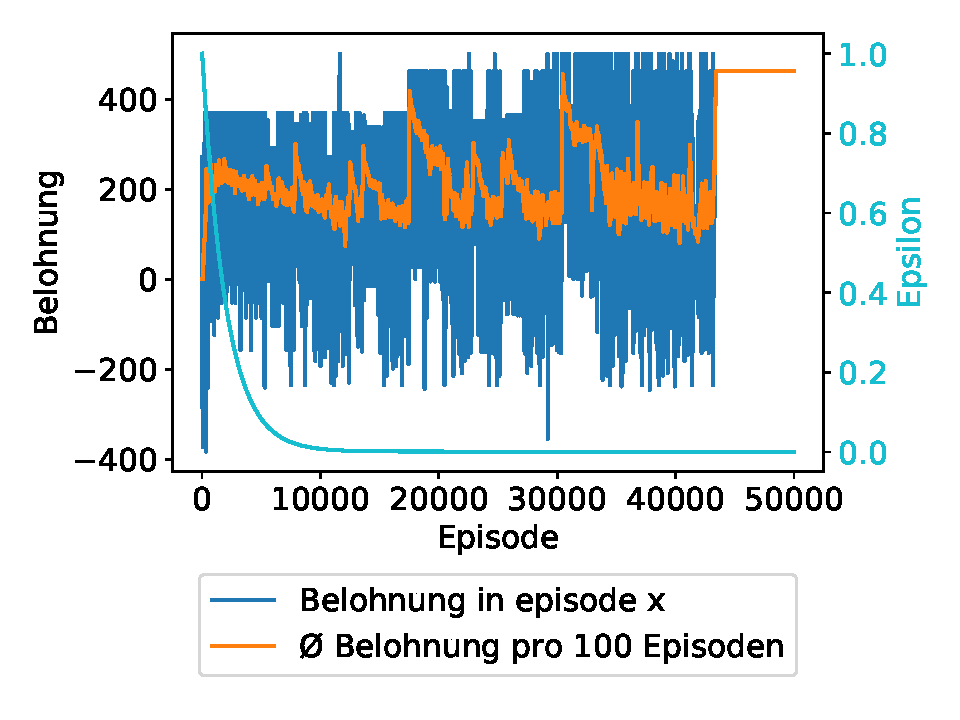
\includegraphics[width=\textwidth]{q_learning/figure_epsilon_in_reward_2.pdf}
        \caption{Graph so wie in \ref{img:graphQBest}}
        \label{img:graphQEpsInRew}
    \end{subfigure}
    \begin{subfigure}[b]{0.49\textwidth}
        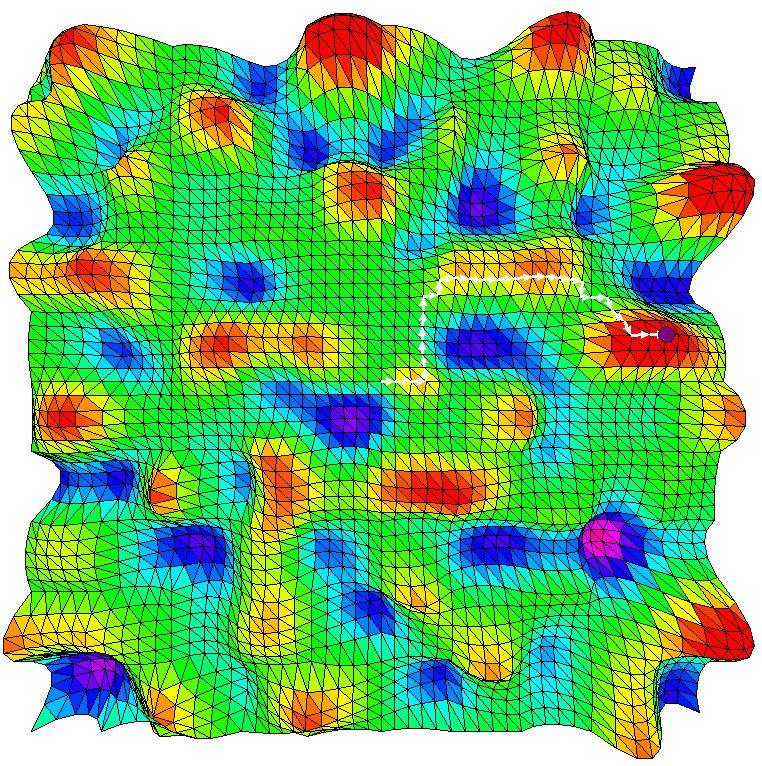
\includegraphics[width=\textwidth]{q_learning/terrain_epsilon_in_reward.JPG}
        \caption{Bester Pfad des Agenten nach dem Training}
        \label{img:pathQEpsInRew}
    \end{subfigure}
    \caption{Trainingsergebnisse mit Erkundungsstrategie codiert im Reward}
\end{figure}
Wichtig ist es an dieser Stelle zu erwähnen, dass der Graph \ref{img:graphQEpsInRew} die unverfälschte, von der Umgebung gelieferte Belohnung vor der Modifikation zeigt, da uns der tatsächliche Lernfortschritt des Agenten interessiert und man diesen sonst nicht mit den Ergebnissen anderen Experimente vergleichen könnte. Es fällt deutlich auf, dass der Lernprozess hier anders verläuft als in \ref{img:graphQBest}. Wir erhalten keine saubere Lernkurve. Trotzdem erreicht der Agent einen maximalen moving average von etwas über 462. Zum Vergleich: Der maximale moving average von \ref{img:graphQBest} liegt bei etwas über 497. Die Q-table dieses Experiments enthält 850 von 10000 mit Null belegte Einträge.

Abbildung \ref{img:pathQEpsInRew} zeigt den Pfad des Agenten bei Verwendung der erzeugten Q-table. Er findet zwar nicht den höchsten Punkt, erklimmt aber dennoch einen hohen Berg, welcher sich nicht in unmittelbarer Nähe des Startzustands befindet. Die Strategie hat also zur besseren Erkundung der Umgebung beigetragen.

Wiederholt man das Experiment 20 mal, so lässt sich der folgende Durchschnitt mit Standartabweichung berechnen:
\begin{figure}[H]
    \centering
    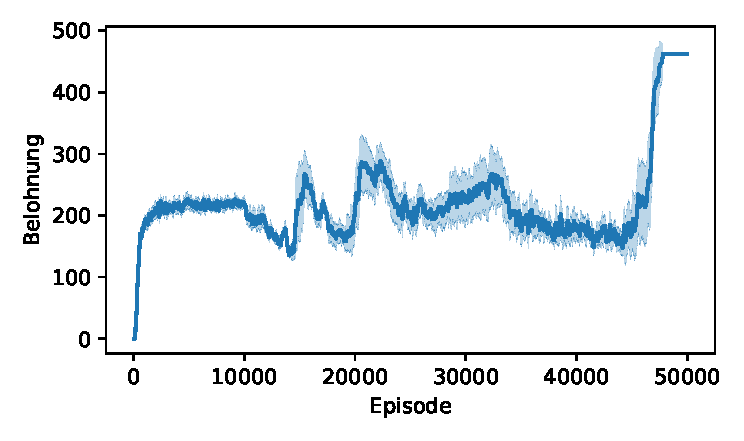
\includegraphics{q_learning/figure_epsilon_in_reward_mean.pdf}
    \caption{Trainingsergebnisse mit Erkundungsstrategie codiert im Reward nach 20 Wiederholungen. Graph so wie in \ref{img:graphQEpsComp}.} \label{img:graphQEpsInRewMean}
\end{figure}
Der Agent benötigt mit 50000 Episoden sehr lange, um seinen Höchstwert zu erreichen. Dieser scheint sich auch nach circa Episode 47 nicht mehr zu verändern, was vermutlich darauf zurückzuführen ist, dass der Agent immer greedy agiert und zu diesem Zeitpunkt kein besserer ihm bekannter Pfad mehr existiert. Verglichen mit dem Agenten ohne Erkundungsstrategie lässt sich festhalten, dass die Modifikation der Belohnung in diesem Fall eine höheren Ertrag sowie eine bessere Erkundung der Umgebung bewirkt hat. Diese Strategie dauert allerdings deutlich länger und liefert etwas weniger Ertrag als die klassische $ \epsilon $-greedy Strategie.
% \begin{minted}{python}
% params = Parameters(
%         num_episodes=100,
%         max_steps_per_episode=20,

%         learning_rate=0.5,
%         discount_rate=0.99,

%         start_exploration_rate=1,
%         max_exploration_rate=1,
%         min_exploration_rate=0.01,
%         exploration_decay_rate=0.1,

%         rewards_all_episodes=[],
%         max_rewards_all_episodes=[],
%     )
% \end{minted}

% https://github.com/simoninithomas/Deep_reinforcement_learning_Course/tree/master/Q%20learning/FrozenLake

% \begin{figure}[h]
%     \centering
%     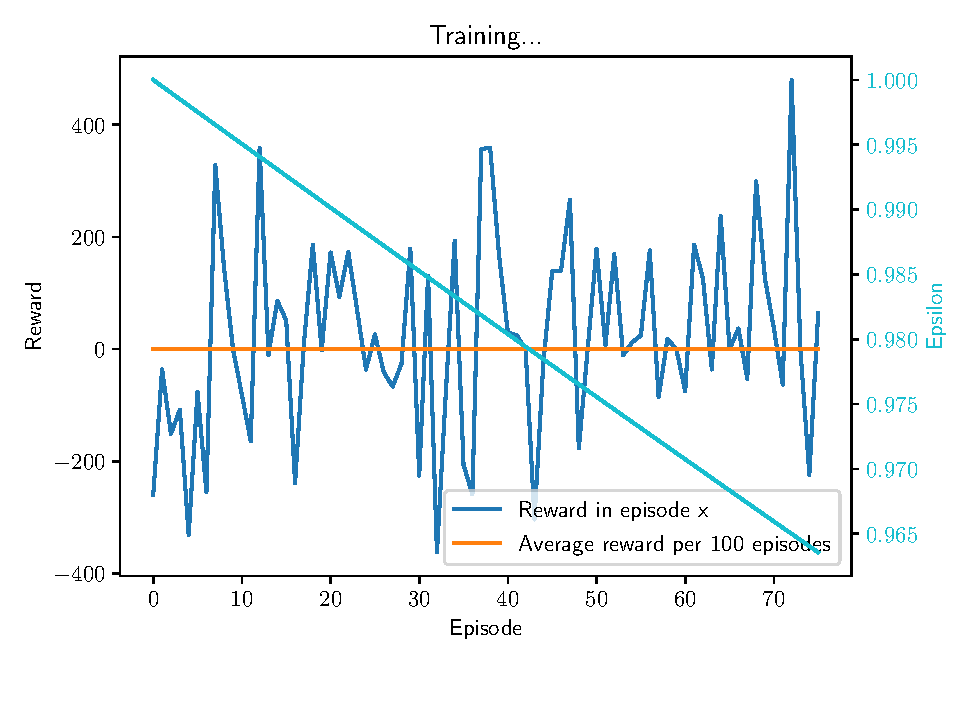
\includegraphics[width=\textwidth]{plot_test.pdf}
%     \caption{Visualisierung von zweidimensionaler Perlin Noise} \label{img:terrainMain}
% \end{figure}

% \begin{align}
%     \mathcal{F}(\theta) & = H(A|S,Z) - H(Z|S) + H(Z) \nonumber\\
%     & = H(A|S,Z) + E_{z \sim p(z), s \sim \pi(z)}(log\ p(z | s)) - E_{z \sim p(z)}(log\ p(z)) \label{eq:objective_2}\\
%     & \ge H(A|S,Z) + E_{z \sim p(z), s \sim \pi(z)}(log\ q_\phi(z | s) - log\ p(z)) \stackrel{\triangle}{=} \mathcal{G}(\theta, \phi) \nonumber
% \end{align}


% Grid, auf dem sich der Agent bewegen
% Perlin Noise
% 
% Color-coded: Rot ist hoch, blau ist tief
% 

%% Ziel des Agenten

%% Agent mit Q-Table

%% Agent mit Neuronalem Netz

%% Ergebnisse

% \begin{minted}{python}
%     import numpy as np
      
%     def incmatrix(genl1,genl2):
%         m = len(genl1)
%         n = len(genl2)
%         M = None #to become the incidence matrix
%         VT = np.zeros((n*m,1), int)  #dummy variable
      
%         #compute the bitwise xor matrix
%         M1 = bitxormatrix(genl1)
%         M2 = np.triu(bitxormatrix(genl2),1) 
      
%         for i in range(m-1):
%             for j in range(i+1, m):
%                 [r,c] = np.where(M2 == M1[i,j])
%                 for k in range(len(r)):
%                     VT[(i)*n + r[k]] = 1;
%                     VT[(i)*n + c[k]] = 1;
%                     VT[(j)*n + r[k]] = 1;
%                     VT[(j)*n + c[k]] = 1;
      
%                     if M is None:
%                         M = np.copy(VT)
%                     else:
%                         M = np.concatenate((M, VT), 1)
      
%                     VT = np.zeros((n*m,1), int)
      
%         return M
%     \end{minted}

%% Deep-Q-Learning Experiments
\section{Deep-Q-Learning Experimente}
Wir wollen die Implementierung aus Kapitel \ref{sec:deepQImplementation} nun für einige Experimente mit Deep-Q-Agenten nutzen. Ziel ist es zunächst, eine geeignete Aufgabe für den Agenten zu finden, welche anschließend für den Vergleich unterschiedlicher Lernstrategien dienen soll.

\subsection{Erste Experimente} \label{sec:deepQFirstExperiments}
\paragraph{Ausgangsexperiment}
Das DQN erhält als Eingabe die aktuelle Position des Agenten in Form einer x- und einer y-Koordinate. Diese beschreiben in diesem Experiment den Zustand des Agenten. Die Mitte der Landschaft hat die Koordinaten (0, 0). Dies ist ebenfalls der Startpunkt des Agenten. Als Belohnung erhält der Agent wie in Kapitel \ref{sec:qLearningExperiments} die Differenz der Höhe des Folgezustands und des aktuellen Zustands. Die Hyperparameter werden wie folgt belegt:
\begin{minted}{python}
params = DeepQParameters(
            num_episodes=10000,
            max_steps_per_episode=100,
            replay_buffer_size=20000,
            batch_size=32,
            learning_rate=0.001,
            discount_rate=0.999,
            target_update=25,
            start_exploration_rate=1,
            max_exploration_rate=1,
            min_exploration_rate=0.001,
            exploration_decay_rate=0.001,
            # ... Rest wird erst während des Trainings belegt
        )
\end{minted}
Damit einzelne Beobachtungen nicht zu einer völligen Veränderung der Gewichte im DQN führen, ist die \mintinline{python}{learning_rate} im Vergleich zum Training mit der Q-table sehr klein.
\begin{figure}[h!]
    \centering
    \begin{subfigure}[b]{0.49\textwidth}
        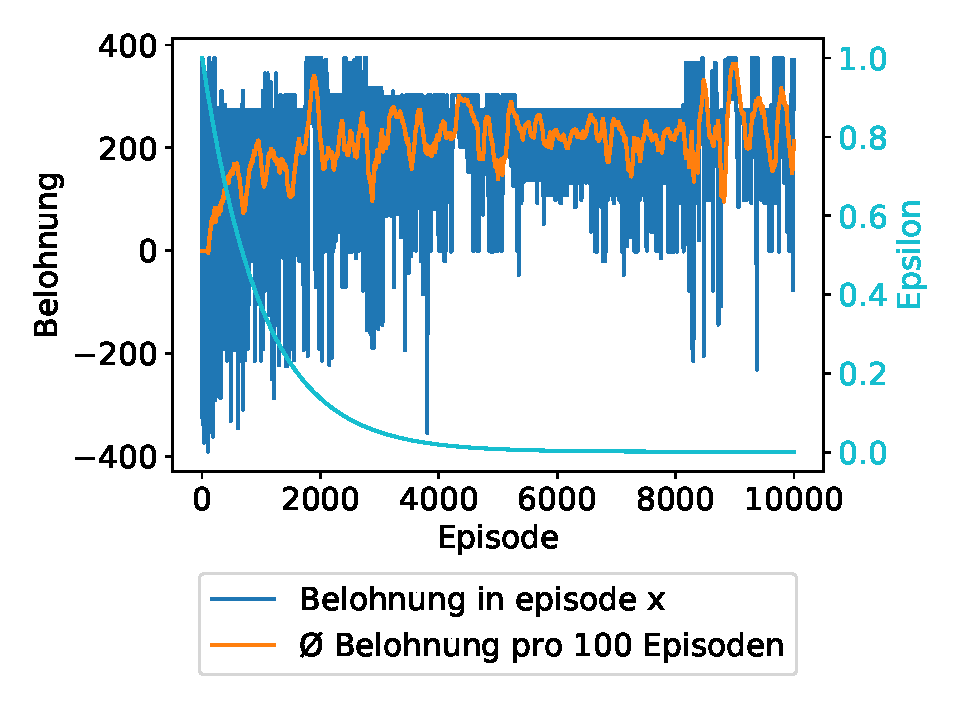
\includegraphics[width=\textwidth]{deep_q_learning/figure_simple.pdf}
        \caption{Graph so wie in \ref{img:graphQBest}}
        \label{img:graphDeepQSimple}
    \end{subfigure}
    \begin{subfigure}[b]{0.49\textwidth}
        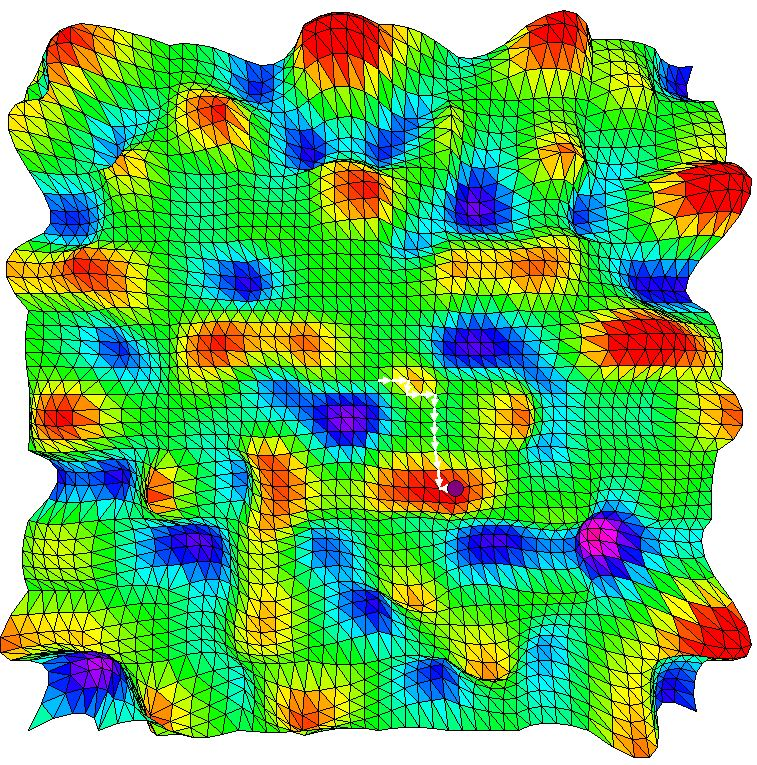
\includegraphics[width=\textwidth]{deep_q_learning/terrain_path_simple.JPG}
        \caption{Bester Pfad des Agenten nach dem Training}
        \label{img:pathDeepQSimple}
    \end{subfigure}
    \caption{Ergebnisse des ersten Experiments mit DQN}
\end{figure}

Der Agent scheint mit diesen Informationen noch nicht viel anfangen zu können. Der Graph in Abbildung \ref{img:graphDeepQSimple} zeigt, dass der moving average Wert (orange) über die komplette Trainingszeit sehr inkonsistent ist. Außerdem liegt er größtenteils deutlich unter dem möglichen Höchstwert. Dies lässt sich daran erkennen, dass die blaue Linie -- also die Belohnung der einzelnen Episoden -- teilweise fast bis 400 geht, der moving average diesen aber nur wenige Male fast erreicht. Außerdem wissen wir aus Kapitel \ref{sec:qLearningExperiments}, dass definitiv ein Wert von 497 möglich ist. In Abbildung \ref{img:pathDeepQSimple} ist zu erkennen, welchen Pfad der Agent unter Verwendung des aus dem Training resultierenden Netzes zurücklegt. Er bewegt sich auf einen Gipfel, welcher sich in der Nähe des Startzustands befindet. Optimal wäre jedoch der Gipfel ganz oben in der Mitte.

Das DQN liefert hier also kein sonderlich gutes Ergebnis. Dies könnte daran liegen, dass der Agent keinerlei Information über die Höhe seiner Zustände hat, von denen seine erhaltene Belohnung und die Erfüllung der Aufgabe ja stark abhängt.

\paragraph{Anpassung der Parameter}
Wir passen also die Werte an, die einen Zustand beschreiben und fügen die Höhe des aktuellen Zustands, sowie die der umliegenden Zustände hinzu. Das DQN erhält also nun als Eingabe sieben Werte (x- und y-Koordinate, eigene Höhe und die Höhe der vier umliegenden Felder).

Das letzte Training hat für die 10000 Episoden etwas über eineinhalb Stunden gedauert\footnote{Die Experimente wurden auf einer Nvidia RTX 2060 durchgeführt}. Wir suchen eine Aufgabe, die für den Vergleich unterschiedlicher Lernstrategien genutzt werden soll und wollen für jede Strategie eine Experimentreihe durchlaufen, um eine statistische Auswertung zu ermöglichen. Diese sollten in zumutbarer Zeit durchführbar sein. Daher ist es wichtig, die Trainingszeit für einzelne Experimente zu reduzieren. 

Wir reduzieren daher die Episodenanzahl \mintinline{python}{num_episodes} auf 1500. Dementsprechend muss auch die \mintinline{python}{exploration_decay_rate} angepasst werden. Wir setzen diese auf 0.005.
\begin{figure}[h!]
    \centering
    \begin{subfigure}[b]{0.49\textwidth}
        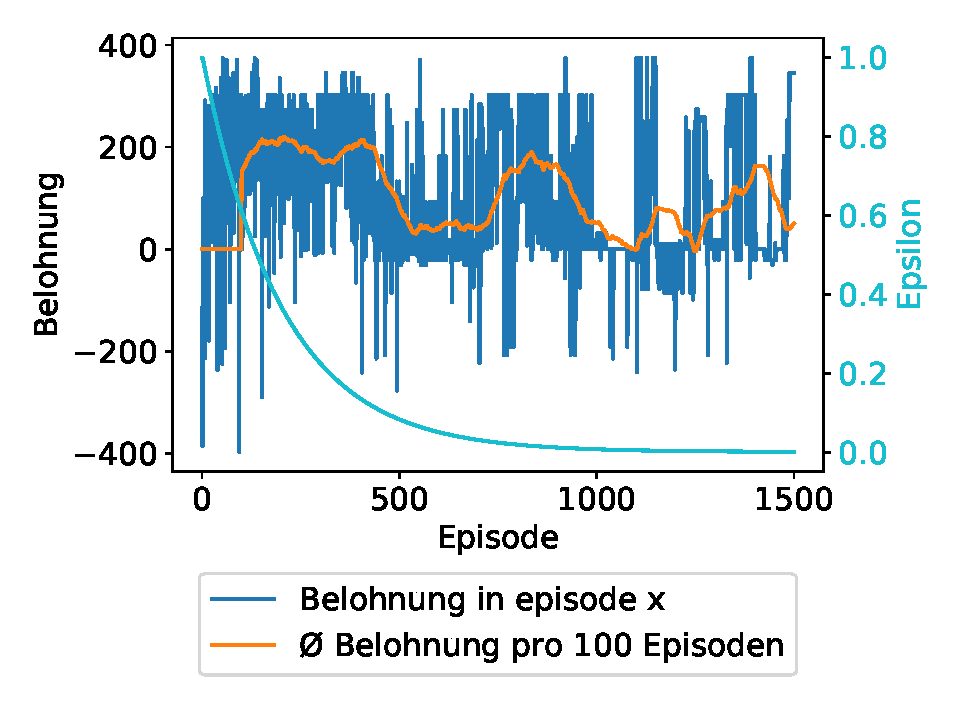
\includegraphics[width=\textwidth]{deep_q_learning/figure_height_in_state.pdf}
        \caption{Graph so wie in Abbildung \ref{img:graphQBest}}
        \label{img:graphDeepQHeightInState}
    \end{subfigure}
    \begin{subfigure}[b]{0.49\textwidth}
        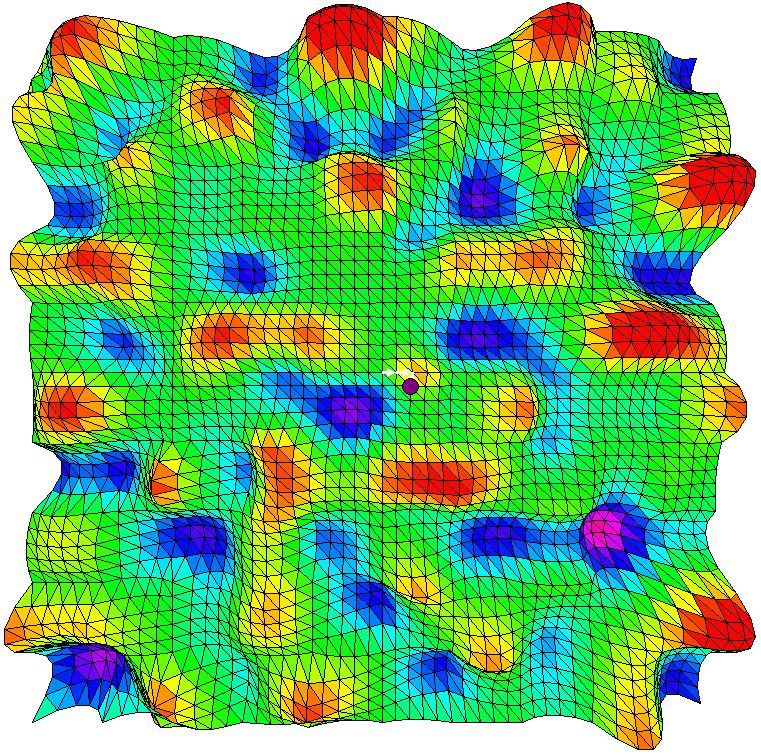
\includegraphics[width=\textwidth]{deep_q_learning/terrain_path_height_in_state.JPG}
        \caption{Bester Pfad des Agenten nach dem Training}
        \label{img:pathDeepQHeightInState}
    \end{subfigure}
    \caption{Ergebnisse mit angepassten Parametern}
\end{figure}
In Abbildung \ref{img:pathDeepQHeightInState} lässt sich schnell erkennen, dass das Trainingsergebnis auch hier nicht zufriedenstellend ist. Der Agent bewegt sich nur ein paar Felder weit zu einem nahe gelegenen, sehr kleinen Hügel. Der moving average in Abbildung \ref{img:graphDeepQHeightInState} zeigt auch keinen gewünschten Trainingsverlauf wie beispielsweise in Abbildung \ref{img:graphQBest}. Lediglich die Trainingsdauer hat sich wie erwartet verringert.

\paragraph{Zufällige Startposition}
Wir werden daher unseren Ansatz etwas verändern. Die Startposition wird zu Beginn jeder Episode zufällig gewählt. Das DQN erhält außerdem statt der absoluten Position im Grid die relative Position zum Startpunkt. Das bedeutet, dass dieser immer die Koordinaten (0, 0) besitzt. Dies soll die Abhängigkeit von einem immer gleichen Startzustand aufbrechen und die Aufgabe interessanter machen.
\begin{figure}[h!]
    \centering
    \begin{subfigure}[b]{0.49\textwidth}
        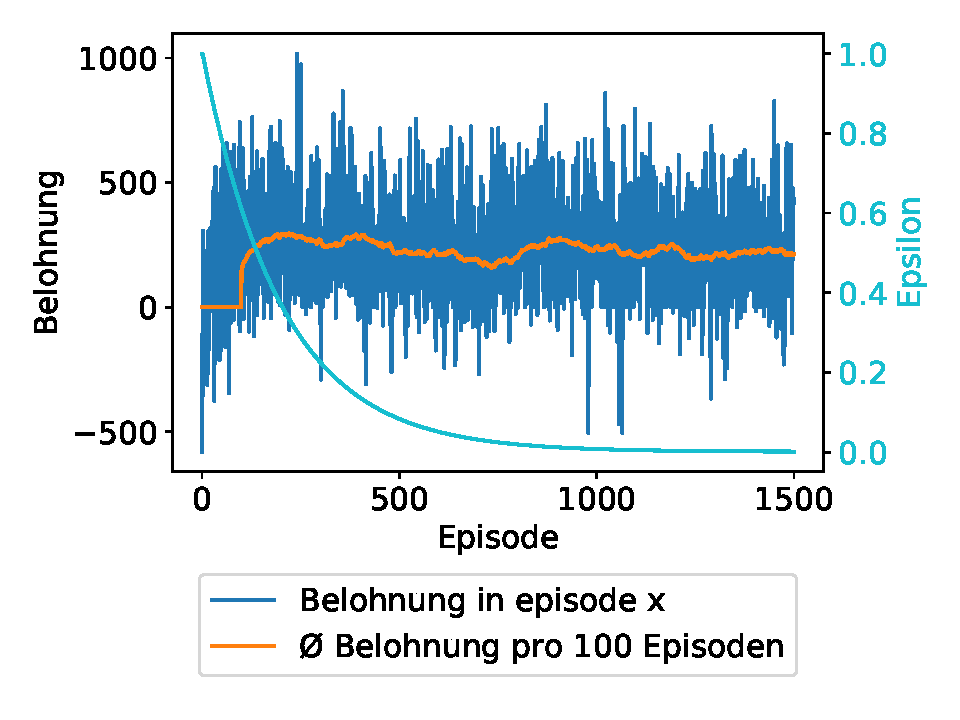
\includegraphics[width=\textwidth]{deep_q_learning/figure_random_spawn.pdf}
        \caption{Graph so wie in Abbildung \ref{img:graphQBest}}
        \label{img:graphDeepQRandomSpawn}
    \end{subfigure}
    \begin{subfigure}[b]{0.49\textwidth}
        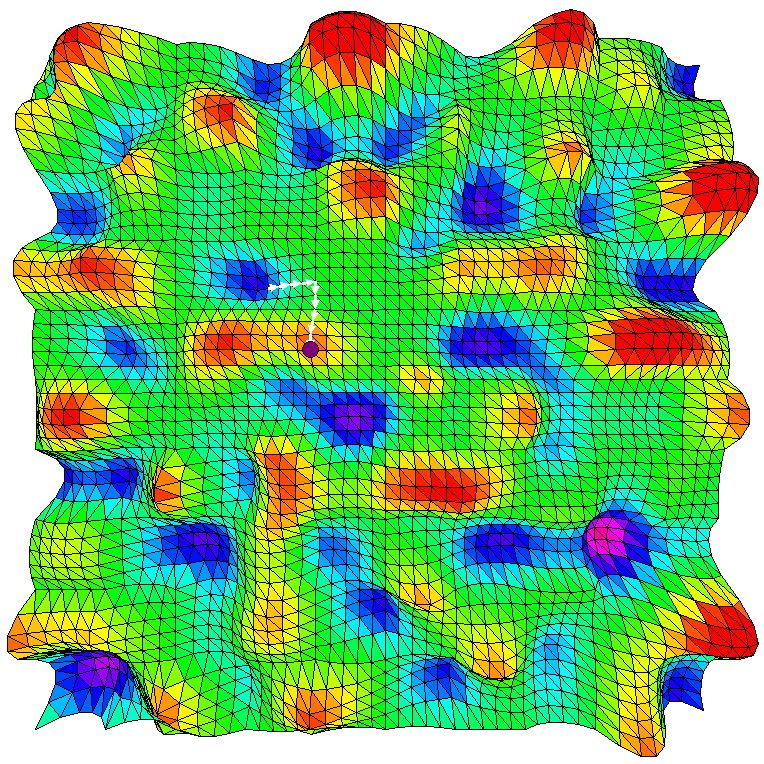
\includegraphics[width=\textwidth]{deep_q_learning/terrain_path_random_spawn.JPG}
        \caption{Bester Pfad des Agenten nach dem Training}
        \label{img:pathDeepQRandomSpawn}
    \end{subfigure}
    \caption{Ergebnisse mit zufälliger Startposition}
\end{figure}
Der Agent läuft nun von seiner Startposition aus so lange in die Richtung eines höheren Punktes, bis es nicht mehr weiter nach oben geht. Einer dieser möglichen Pfade ist in Abbildung \ref{img:graphDeepQRandomSpawn} zu sehen. Das ist schon mal ein Schritt in die richtige Richtung. Die Aufgabe ist allerdings zu einfach. Im Graph in Abbildung \ref{img:graphDeepQRandomSpawn} lässt sich erkennen, dass der Großteil des Lernvorgangs bereits vor der 100-Epsioden-Marke passiert. Dies ist nicht optimal für unsere Zwecke, da wir erst ab Episode 100 den moving average und damit unsere Hauptvergleichsquelle verfolgen können.

Das neue Ziel soll daher sein, dass der Agent nicht nur nach oben läuft, sondern einen möglichst hohen Punkt in der Nähe des Startpunktes findet. Zu diesem Zweck erweitern wir die Eingaben, die das DQN bekommt. Wir übergeben nun die Höhe und die relative Position des in diesem Zeitschritt bisher höchsten besuchten Feldes. Außerdem wird die Anzahl der übrigen und der maximalen Zeitschritte angefügt. Dies soll in der Theorie dazu führen, dass der Agent seine Umgebung erkundet, solange noch genügend Zeit ist. Gegen Ende der Episode sollte er dann zum bisher höchsten bekannten Gipfel laufen.

\begin{figure}[h!]
    \centering
    \begin{subfigure}[b]{0.49\textwidth}
        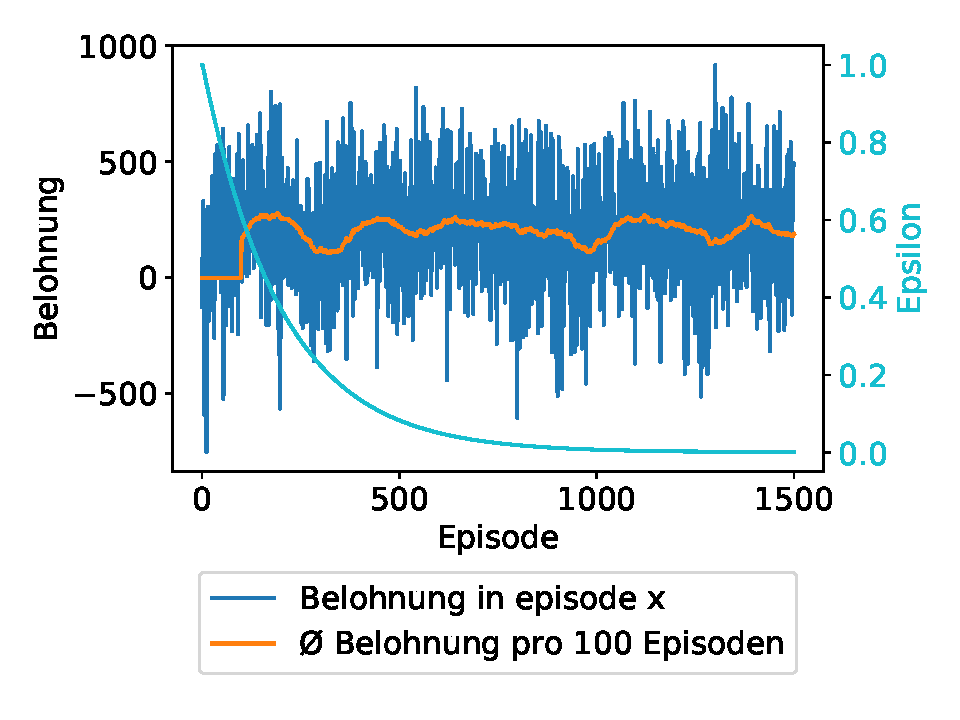
\includegraphics[width=\textwidth]{deep_q_learning/figure_random_spawn_2.pdf}
        \caption{Graph so wie in Abbildung \ref{img:graphQBest}}
        \label{img:graphDeepQRandomSpawn2}
    \end{subfigure}
    \begin{subfigure}[b]{0.49\textwidth}
        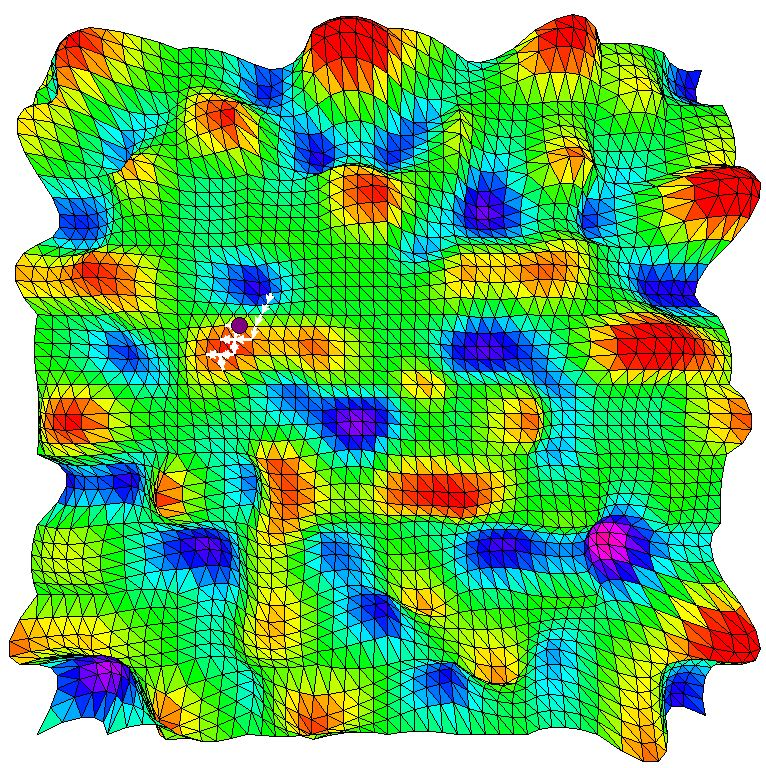
\includegraphics[width=\textwidth]{deep_q_learning/terrain_path_random_spawn_2.JPG}
        \caption{Bester Pfad des Agenten nach dem Training}
        \label{img:pathDeepQRandomSpawn2}
    \end{subfigure}
    \caption{Ergebnisse mit zusätzlichen Inputs}
\end{figure}

Das Ergebnis ist ähnlich wie das des vorangegangenen Experiments. Zum besseren Vergleich haben wir für die Darstellung in Abbildung \ref{img:pathDeepQRandomSpawn2} denselben Startpunkt gewählt wie in Abbildung \ref{img:pathDeepQRandomSpawn}. Der Agent orientiert sich tatsächlich hin zum etwas höheren Gipfel und scheint in einem sehr kleinen Umkreis die Umgebung zu erkunden, versäumt es aber am Ende auf dem höchsten Punkt aufzuhören. Dies kann  daran liegen, dass sich der Agent in jedem Zeitschritt bewegen muss und auf diese Weise nicht die Möglichkeit besitzt, genau auf dem höchsten Feld aufzuhören. Die Farbcodierung der Landschaft verrät uns allerdings, dass das Feld links oder unterhalb des vorletzten Schritts höher gelegen ist als das gewählte obere Feld. Viel wichtiger ist jedoch, dass der Graph in Abbildung \ref{img:graphDeepQRandomSpawn2} keinen wirklichen Trainingsfortschritt zeigt. Der moving average pendelt hier grob um denselben Wert und zeigt keinerlei Verbesserung des Agenten über längere Zeit. Auch dieser Ansatz ist also für unsere Zwecke nicht geeignet.

\paragraph{Neudefinition des Lernziels}
Aufgrund der Misserfolge mit dem Finden von hohen Gipfeln wollen wir nun versuchen, ein anderes Ziel zu erarbeiten. Die neue Idee ist, dass der Agent so viele Felder wie möglich besuchen soll, sich dabei aber so wenig wie möglich vom Startfeld entfernt. Wir erhoffen uns hiervon, dass die quasi gegensätzlichen Ziele zu interessanten Ergebnissen führen und für ein DQN ein angemessenes Problem darstellen.

Um dieses Verhalten zu erreichen, werden sowohl die Beschreibung eines Zustands als auch die Belohnung stark angepasst. Die Belohnung setzt sich aus den beiden Aufgaben zusammen und sieht in etwa so aus:
\begin{minted}{python}
reward = (NEW_POINT_REWARD if is_new_point else 0) -\
         (DISTANCE_MULTIPLIER * distance_from_spawn)
\end{minted}
Der erste Part gibt den fixen Belohnungswert \mintinline{python}{NEW_POINT_REWARD} aus, falls das Feld vom Agenten noch nicht besucht wurde, ansonsten null. Davon wird dann die Distanz vom Startzustand abgezogen. Auf diese Weise erhält der Agent höhere Strafen je weiter er sich von diesem entfernt. Die Distanz wird davor noch mit einem ebenfalls fixen Wert \mintinline{python}{DISTANCE_MULTIPLIER} multipliziert. Die beiden fixen Werte (im Folgenden \textit{Belohnungsparameter} genannt) sollen als Stellschrauben dienen, um die richtige Gewichtung der beiden Ziele zu finden.

Als nächstes passen wir die Werte an, die einen Zustand beschreiben. Nicht mehr benötigt werden die Daten über die Höhe des eigenen und der umliegenden Felder. Stattdessen wird für jede angrenzende Position ein positiver Wert geliefert, wenn der Agent diese noch nicht besucht hat. Hat er das Feld schon besucht, so entspricht dieser Wert 0. Befindet sich der Agent am Rand der Landschaft und eines der angrenzenden Felder somit außerhalb des Grids, so wird der entsprechende Wert mit einer negativen Zahl belegt. Die Höhe der positiven und der negativen Wert lässt sich ebenfalls über einen fixen Parameter festlegen.
\begin{figure}[h!]
    \centering
    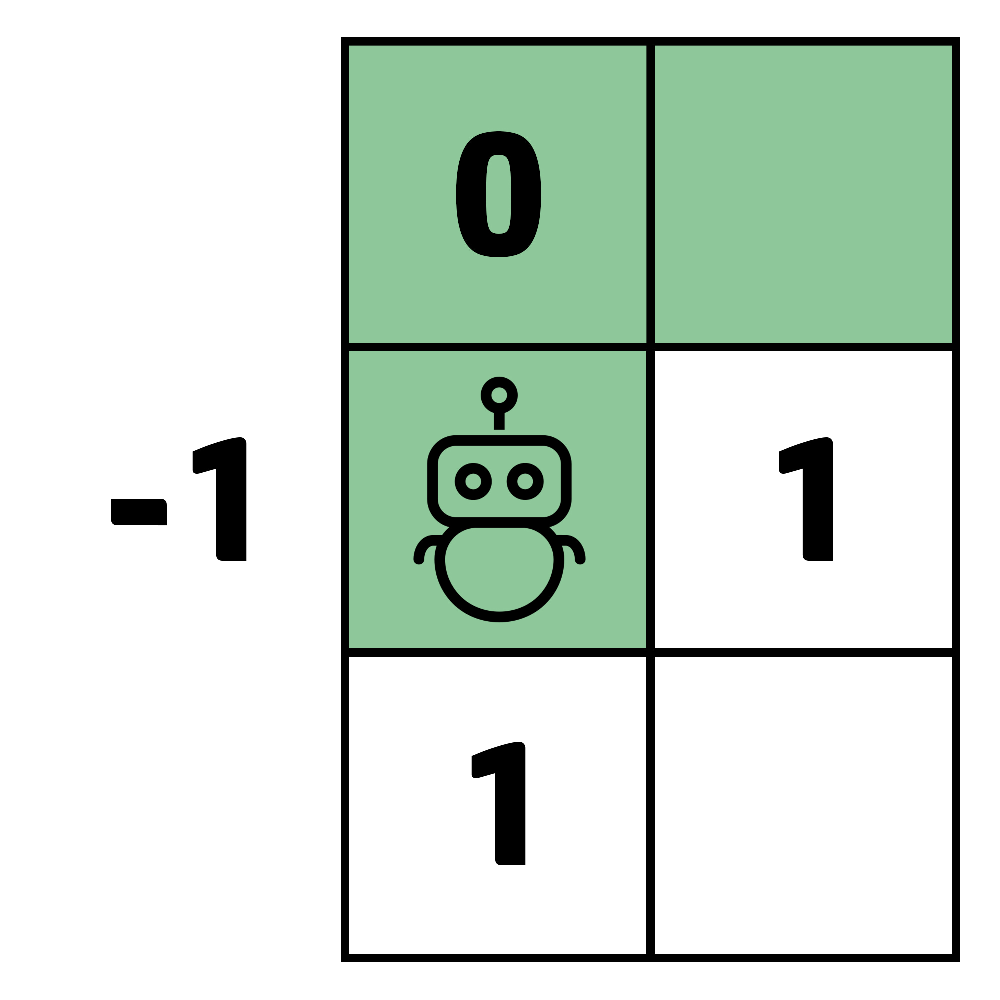
\includegraphics[width=0.3\textwidth]{state_visualisation.pdf}
    \caption{Visualisierung der Inputs des Agenten abhängig von den angrenzenden Positionen im Raster} \label{img:stateVisualisation}
\end{figure}
Abbildung \ref{img:stateVisualisation} zeigt ein Beispiel, wie die entsprechenden Werte ohne Multiplikator aussehen können. Das Raster stellt einen kleinen Ausschnitt des Landschaft-Grids dar. Die grünen Felder hat der Agent bereits besucht. Das DQN erhält für das obere, bereits gesehene Feld also den Wert 0. Die beiden unerforschten Positionen rechts und unten liefern jeweils einen positiven Wert -- in diesem Fall ohne einen Multiplikator also den Wert 1. Da die Position links des Agenten außerhalb des Grids liegt, ist diese mit dem Wert -1 belegt.

Die Werte bezüglich den Zeitschritten aus dem vorherigen Experiment sind ebenfalls enthalten. Insgesamt besteht ein Zustand jetzt also aus 8 Werten: Die relative Position (2), die Information über die anliegenden Positionen (4) und die Werte der übrigen beziehungsweise maximalen Zeitschritte (2).
\begin{figure}[h!]
    \centering
    \begin{subfigure}[b]{0.59\textwidth}
        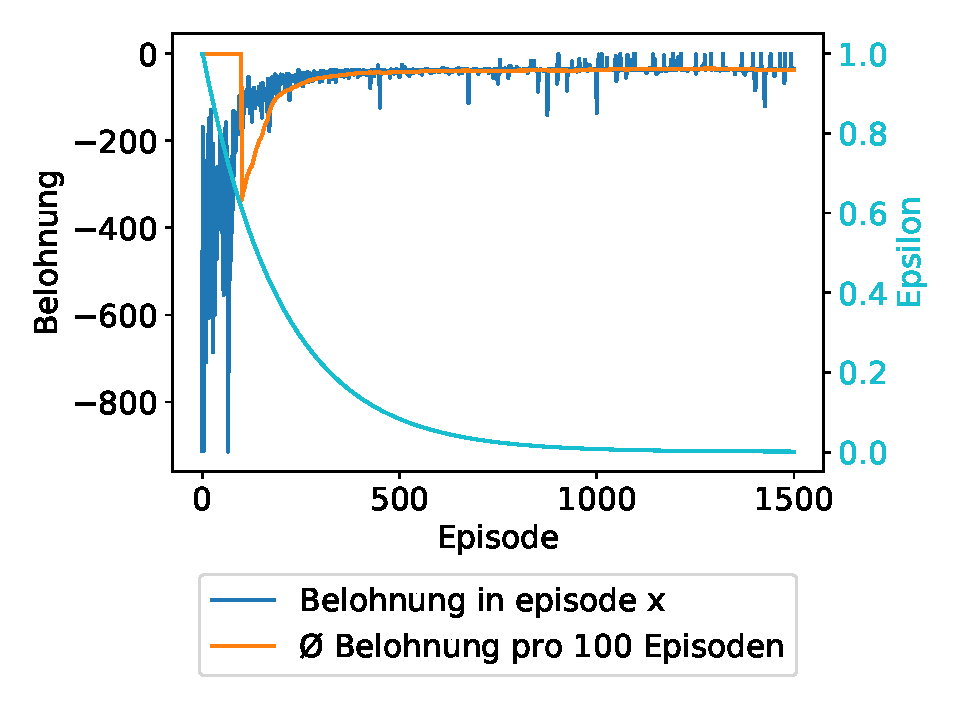
\includegraphics[width=\textwidth]{deep_q_learning/figure_random_spawn_spiral_1.pdf}
        \caption{Graph so wie in Abbildung \ref{img:graphQBest}}
        \label{img:graphDeepQRandomSpawnSpiral1}
    \end{subfigure}
    \begin{subfigure}[b]{0.4\textwidth}
        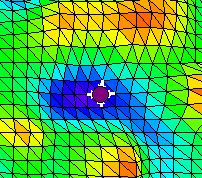
\includegraphics[width=\textwidth]{deep_q_learning/terrain_path_random_spawn_spiral_1_detail.JPG}
        \caption{Bester Pfad des Agenten nach dem Training}
        \label{img:pathDeepQRandomSpawnSpiral1}
    \end{subfigure}
    \caption{Ergebnisse nach Neudefinition des Lernziels}
\end{figure}
Der Graph in Abbildung \ref{img:graphDeepQRandomSpawnSpiral1} zeigt wieder die Trainingsergebnisse der 1500 Episoden an. Am moving average lässt sich diemal ein sauberer Lernfortschritt erkennen. Die durchschnittliche Belohnung steigt bis circa Episode 400 stark an und flacht dann langsam ab. Dieser Verlauf ist zunächst zufriedenstellend. Weniger zufriedenstellend ist allerdings das Verhalten, welches der Agent unter Verwendung des erlernten DQNs zeigt. Wie in Abbildung \ref{img:pathDeepQRandomSpawnSpiral1} zu sehen ist, bewegt sich der Agent von seiner Startposition aus lediglich ein Feld in jede Richtung und springt dann nur noch hin und her.
An dieser Stelle kommen unsere Belohnungsparameter ins Spiel. Da es dem Agenten aktuell wichtiger zu sein scheint, sich so wenig wie möglich vom Startpunkt zu entfernen, setzen wir den \mintinline{python}{NEW_POINT_REWARD} auf 10.
\begin{figure}[h!]
    \centering
    \begin{subfigure}[b]{0.59\textwidth}
        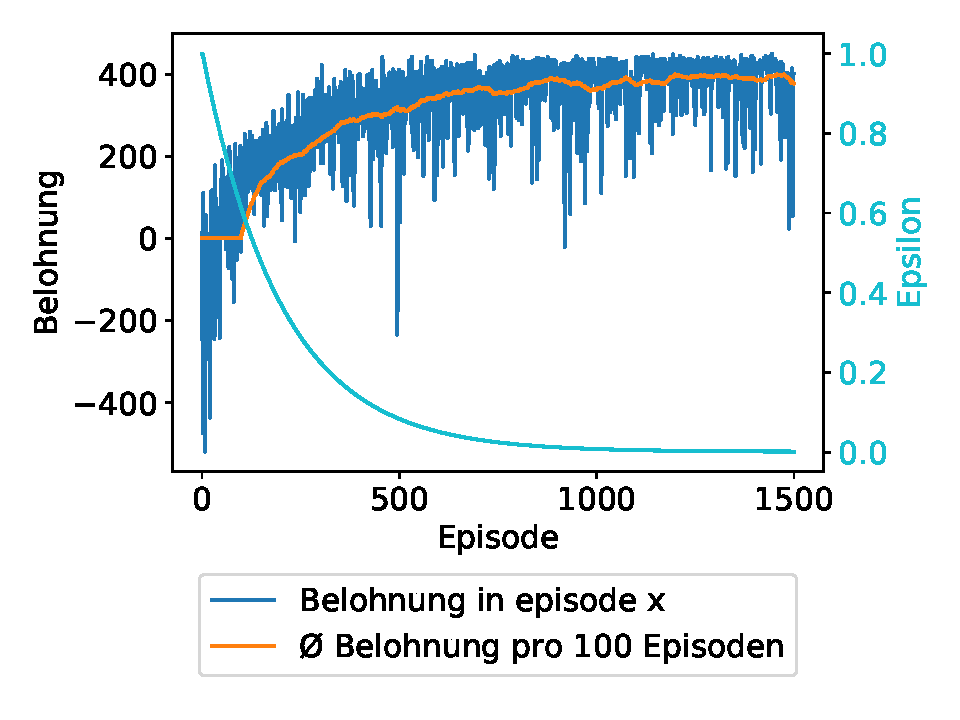
\includegraphics[width=\textwidth]{deep_q_learning/figure_random_spawn_spiral_2.pdf}
        \caption{Graph so wie in Abbildung \ref{img:graphQBest}}
        \label{img:graphDeepQRandomSpawnSpiral2}
    \end{subfigure}
    \begin{subfigure}[b]{0.4\textwidth}
        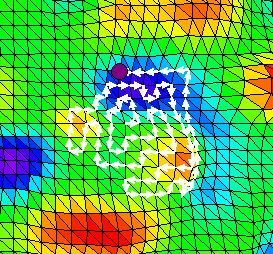
\includegraphics[width=\textwidth]{deep_q_learning/terrain_path_random_spawn_spiral_2_detail.JPG}
        \caption{Bester Pfad des Agenten nach dem Training}
        \label{img:pathDeepQRandomSpawnSpiral2}
    \end{subfigure}
    \caption{Ergebnisse mit größerem \mintinline{python}{NEW_POINT_REWARD}}
\end{figure}
Dies hat einen sehr positiven Einfluss auf das Ergebnis. Abbildung \ref{img:pathDeepQRandomSpawnSpiral2} stellt wieder einen Pfad des Agenten nach dem Training dar. Die Startposition liegt hier etwa in der Mitte der abgelaufenen Fläche und der Agent läuft quasi spiralförmig immer weiter von diesem Punkt weg. Für das Lösen der Aufgabe ist das eine sehr gute Strategie, da viele neue Felder besucht werden und die Distanz zum Startpunkt gleichzeitig so gering wie möglich gehalten wird.

Der Graph in Abbildung \ref{img:graphDeepQRandomSpawnSpiral2} zeigt wie im Experiment davor eine schöne Lernkurve, welche zu Beginn des Trainings stark ansteigt und dann langsam abflacht. Aufgrund der höheren Belohnung für neu besuchte Felder verläuft der moving average nun im positiven Bereich.

Aufgrund dieser positiven Resultate mit dem Experiment werden wir diese Aufgabe für die Durchführung der weiteren Experimente nutzen und die Performance der unterschiedlichen Strategien vergleichen.
% Besser sind 2000 Episoden -> Test mit 10 Iterationen aus den Versuchen extrahieren

% test mit standart reward -> Zu einfach
% Stärke von DQN ausnutzen
% Zufälliger Spawn -> relative pos, sonst gleich -> läuft auf nächsten Berg
% Idee: Finde höchsten Berg in unmittelbarer Nähe, TODO State -> läuft trotzdem nur nach oben
% Neue Aufgabe: Decke so viel Fläche wie möglich ab, aber bleibe dabei so Nahe wie möglich am Spawn (eine Art Spirale)
% -> Gut, um Ergebnisse zu vergleichen
% 

\subsection{Experimente mit unterschiedlichen Strategien}
In Abbildung \ref{img:graphDeepQRandomSpawnSpiral2} erkennt man, dass sich der moving average gegen Ende kaum noch verändert. Er steigt allerdings bis kurz davor noch minimal an, weswegen wir die Episodenlänge -- also die Zeitschritte pro Episode -- auf 2000 erhöhen. So soll sich auch bei langsameren Lernkurven der moving average am Ende bei einem Wert eingependelt haben. Es ist außerdem wichtig zu erwähnen, dass für die zufällige Wahl der Startposition für alle Experimentreihen der gleiche Seed benutzt wird. Die zufälligen Spawnpunkte und deren Reihenfolge sind also für alle Experimente gleich und somit besitzen alle die gleichen Voraussetzungen.

\paragraph{Experimentreihe mit den erarbeiteten Parametern}
Wir führen zunächst eine Experimentreihe mit den in Kapitel \ref{sec:deepQFirstExperiments} erarbeiteten Parametern durch. Das Experiment wird wie in Kapitel \ref{sec:qLearningExperiments} 20 Mal wiederholt. Bei den folgenden Graphen handelt es sich -- falls nicht anders angegeben -- immer um den durchschnittlichen moving average Wert und dessen Standardabweichung, welche als leicht transparenten Bereich um die Linie dargestellt wird.
\begin{figure}[h!]
    \centering
    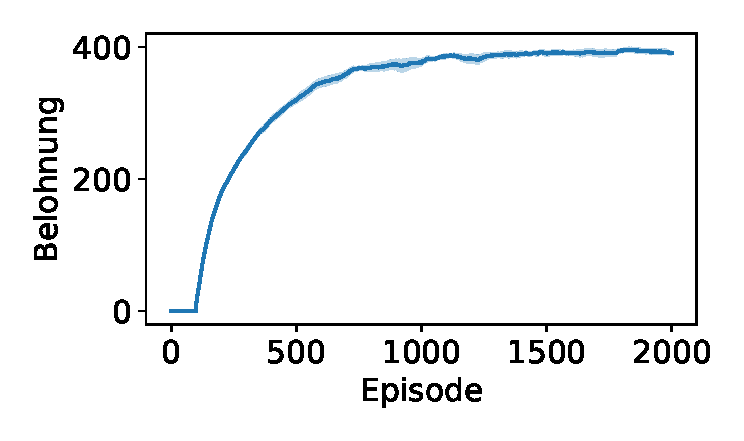
\includegraphics[width=0.5\textwidth]{deep_q_learning/figure_mean_dec_eps_1.pdf}
    \caption{Trainingsergebnisse mit Experiment wie in Abbildung \ref{img:graphDeepQRandomSpawnSpiral2} nach 20 Wiederholungen. Graph so wie in Abbildung \ref{img:graphQEpsComp}.} \label{img:graphDeepQMeanDecEps1}

\end{figure}
Der Lernfortschritt scheint auch über mehrere Experimente hinweg sehr konsistent zu sein. Die Lernkurve verläuft im Graph in Abbildung \ref{img:graphDeepQMeanDecEps1} wie gewünscht anfangs steil und flacht gegen Ende ab. Die Standardabweichung ist zu jedem Zeitpunkt sehr gering, die Ergebnisse der Einzelexperimente unterscheiden sich also nicht stark voneinander. 

\paragraph{Agent ohne Erkundungsstrategie}
Anders verhält es sich beim Training ohne Erkundungsstrategie. Wir setzen hierfür unser $ \epsilon $ konstant auf 0. Der Agent agiert also wieder nur greedy. Auch dieses Experiment wiederholen wir 20 Mal.
\begin{figure}[h!]
    \centering
    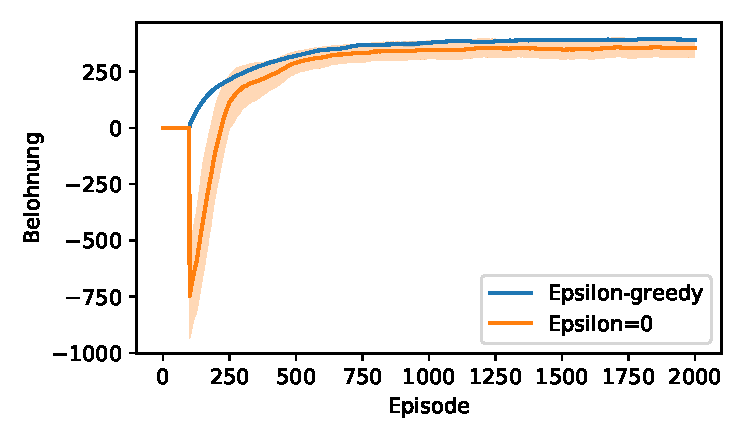
\includegraphics[width=0.8\textwidth]{deep_q_learning/figure_mean_stat_eps_0_vs_dec_eps_1.pdf}
    \caption{Vergleich der Trainingsverläufe mit und ohne $ \epsilon $-greedy Strategie nach jeweils 20 Wiederholungen. Graph so wie in Abbildung \ref{img:graphQEpsComp}.} \label{img:graphDeepQMeanStatEps0VsDecEps1}
\end{figure}
Der Graph in Abbildung \ref{img:graphDeepQMeanStatEps0VsDecEps1} zeigt das Resultat dieses Experiments (orange) und nochmals zum Vergleich das Resultat aus Abbildung \ref{img:graphDeepQMeanDecEps1} (blaue). Es fällt auf, dass die orange Linie wesentlich weiter unten beginnt als die blaue. Das bedeutet, dass der Agent ohne die $ \epsilon $-greedy Strategie langsamer lernt. Außerdem erreicht dieser nicht das gleiche Belohnungsmaximum. Dazu kommt, dass die Standardabweichung auffällig größer ist. Der Lernerfolg ist demnach zusätzlich weniger zuverlässig. So zeigt sich erneut, dass die Verwendung einer Erkundungsstrategie die Performance des Agenten deutlich verbessert.

\paragraph{Konstante $ \epsilon $-Werte}
Als zusätzlichen Vergleich führen wir zwei weitere Experimente mit konstantem $ \epsilon $ durch. Wir setzen hierfür $ \epsilon = 0.2 $ und $ \epsilon = 0.5 $.
\begin{figure}[h!]
    \centering
    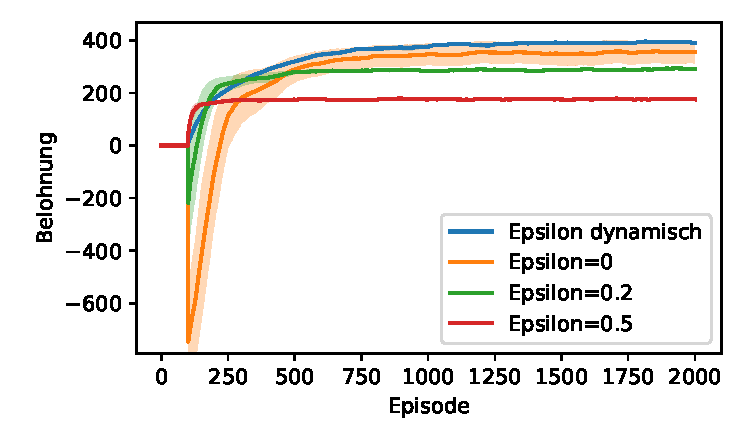
\includegraphics[width=0.8\textwidth]{deep_q_learning/figure_mean_eps_comparison.pdf}
    \caption{Vergleich der Trainingsverläufe mit dynamischem $ \epsilon $ und unterschiedlichen statischen Werten für $ \epsilon $ nach jeweils 20 Wiederholungen. Graph so wie in Abbildung \ref{img:graphQEpsComp}.} \label{img:graphEpsComparison}
\end{figure}
In Abbildung \ref{img:graphEpsComparison} scheint ein Agent ohne Erkundungsstrategie (orange) auf den ersten Blick bessere Ergebnisse zu erzielen als die Agenten mit konstanten $ \epsilon $-Werten (grün und rot). Man darf hierbei allerdings nicht vergessen, dass diese ihr $ \epsilon $ nicht \glqq loswerden \grqq{}, sondern bis zum Ende immer mit der Wahrscheinichkeit $ \epsilon $ eine zufällige Aktion wählen. Da das willkürliche Vorgehen natürlich keine gute Strategie ist, ist in Abbildung \ref{img:graphEpsComparison} auch der moving average der Experimente mit größerem, konstanten $ \epsilon $ geringer. Die tatsächliche Performance des Agenten wird quasi von dem fixen $ \epsilon $ sabotiert. Wir führen daher eine weitere Form der Datendarstellung ein: sogenannte Boxplots.
\begin{figure}[h!]
    \centering
    \begin{subfigure}[b]{0.7\textwidth}
        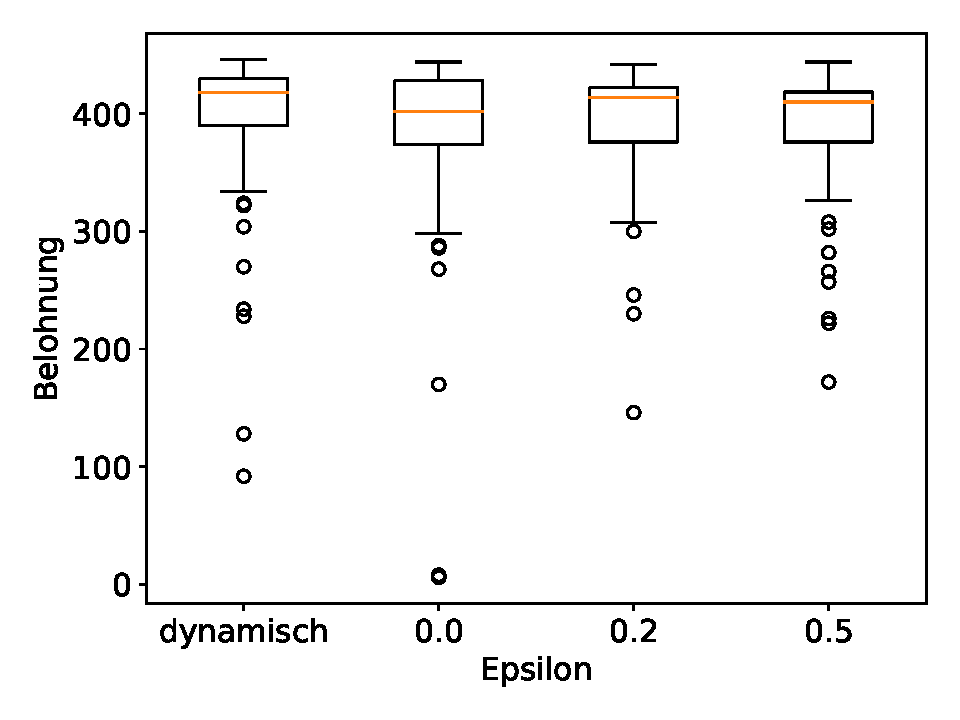
\includegraphics[width=\textwidth]{deep_q_learning/figure_box_eps_comparison.pdf}
        \caption{Kompletter Plot}
        \label{img:graphBoxEpsComparison}
    \end{subfigure}
    \begin{subfigure}[b]{0.7\textwidth}
        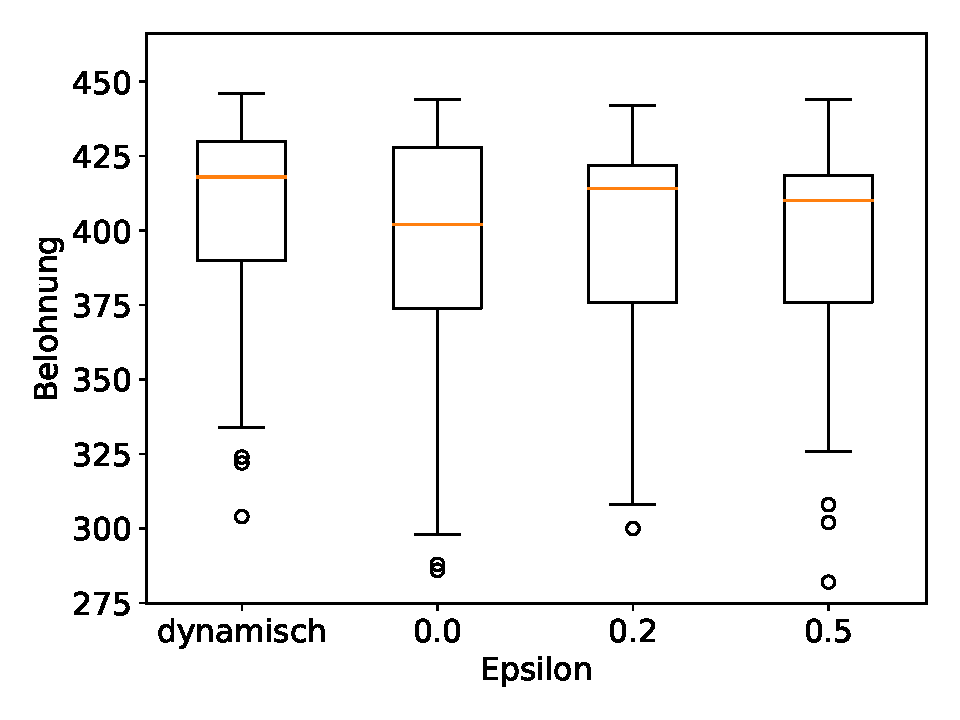
\includegraphics[width=\textwidth]{deep_q_learning/figure_box_eps_comparison_big.pdf}
        \caption{Ausschnitt ohne die unteren Ausreißer}
        \label{img:graphBoxEpsComparisonBig}
    \end{subfigure}
    \caption{Boxplots der Belohnungssummen nach jeweils 100 Durchläufen mit den trainierten DQNs (100 pro Experimentreihe, also bei 20 Iterationen somit 5 Durchläufe pro DQN). y-Achse zeigt die Belohnung, x-Achse beschreibt das betrachtete Experiment. Experimente von links nach rechts: $ \epsilon $ dynamisch, $ \epsilon = 0.0 $, $ \epsilon = 0.2 $, $ \epsilon = 0.5 $}
    \label{img:graphBoxEpsComparisonBoth}
\end{figure}

Die Boxplots sollen das Verhalten des Agenten unter Anwendung des erlernten DQNs beschreiben. Die y-Achse in den Plots in Abbildung \ref{img:graphBoxEpsComparisonBoth} zeigt wieder die Summe der Belohnungen innerhalb einer Episode an. Die x-Achse beschreibt, um welches Experiment es sich handelt, also in diesem Fall welches $ \epsilon $ benutzt wurde. Von links nach rechts sind das in diesem Fall unser dynamisches $ \epsilon $ gefolgt von den drei fixen Werten 0.0, 0.2 und 0.5. Jedes Experiment wurde bisher 20 Mal durchgeführt. Das bedeutet, dass wir für jede Experimentenreihe 20 trainierte DQNs besitzen. Der Agent durchläuft nun mehrere Iterationen, wobei er jedes dieser Netze 5 Mal in der Umgebung anwendet. Pro Experimentreihe erhalten wir also 100 Belohnungssummen, welche wir in einem Boxplot darstellen. Der Seed für die Startposition wird zu Beginn jedes Experiments zurückgesetzt, um gleiche Voraussetzungen zu gewährleisten. Der Graph in Abbildung \ref{img:graphBoxEpsComparison} zeigt die resultierenden Boxplots mit ihren Ausreißern. In Abbildung \ref{img:graphBoxEpsComparisonBig} wurden diese für die bessere Lesbarkeit der Boxplots abgeschnitten.

Es lässt sich zunächst feststellen, dass der Median beim Boxplot des dynamischen $ \epsilon $ den höchsten Wert hat. Ebenso liegen aber auch die anderen Werte, also das 1. Quartil, das 3. Quartil, das Minimum und das Maximum, bei diesem Experiment am höchsten. Es lässt sich also klar sagen, dass ein über Zeit schrumpfendes Epsilon -- also die klassische $ \epsilon $-greedy Strategie -- in der Anwendung bei uns die beste Performance liefert.

Bei den Experimenten mit fixem Epsilon fällt als Erstes auf, dass das Minimum mit steigendem Epsilon immer größer wird. Wir interpretieren dies so, dass die Agenten mit einem größeren Epsilon mehr von ihrer Umgebung erkundet haben und daher für mehr Anwendungsfälle eine bessere Strategie haben. Dass der Median beim Epsilon von 0.5 wieder leicht niedriger ist als bei 0.2 kann eventuell bedeuten, dass ein zu großes Epsilon dazu führt, dass die bereits erkundeten Pfade weniger stark perfektioniert werden. Die Änderung ist allerdings relativ gering. Um hier eine eindeutige Aussage zu treffen bräuchten wir mehr Daten.

Wir haben allerdings einmal mehr gezeigt, dass sich die Erkundungsstrategie auf das Verhalten des Agenten auswirkt.

\subsection{Abbildung einer Erkundungsstrategie über die Modifikation des Rewards} \label{sec:deepQRewardModification}
Im Folgenden soll die Erkundungsstrategie nur über die Reward-Funktion abgebildet werden. Wir modifizieren unseren Agenten also zunächst dahingehend, dass er in jedem Fall greedy agiert. Die Hyperparameter für Epsilon haben also keinen direkten Einfluss mehr auf die Wahl der Aktion. Wir nutzen für die Experimente, falls nicht anders angegeben, die folgenden Hyperparameter:
\begin{minted}{python}
params = DeepQParameters(
            num_episodes=2000,
            max_steps_per_episode=80,
            replay_buffer_size=20000,
            batch_size=32,
            learning_rate=0.001,
            discount_rate=0.999,
            target_update=25,
            start_exploration_rate=1,
            max_exploration_rate=1,
            min_exploration_rate=0.001,
            exploration_decay_rate=0.005,
            # ... Rest wird erst während des Trainings belegt
        )
\end{minted}

\paragraph{Modifizierter Reward mit fixem Faktor}
In Abbildung \ref{img:graphEpsComparison} lässt sich erkennen, dass die Belohnungssumme in einer Episode maximal circa 400 beträgt. Da eine Episode 80 Zeitschritte enthält, bekommt der Agent pro Zeitschritt eine durchschnittliche Belohnung von ungefähr 5. Wir nutzen dieses Wissen, um eine neue Belohnungs-Funktion zu formulieren:
\begin{minted}{python}
modified_reward = (1 - exploration_rate) * reward - exploration_rate * 5
\end{minted}
Ähnlich wie beim Q-Learning-Experiment soll der Agent so zu Beginn negative Belohnungen erhalten, damit er andere Pfade erkundet. Wir lassen den Agenten mit dieser Strategie ebenfalls 20 Mal trainieren. Da bei dieser Belohnugs-Funktion mit den aktuellen Hyperparametern am Anfang nichts von der tatsächlichen Belohnung übrig bleibt und der Agent auf diese Weise eventuell in den ersten Zeitschritten nichts lernt, führen wir noch ein weiteres Experiment durch, dessen Hyperparameter mit \mintinline{python}{start_exploration_rate=0.5} und \mintinline{python}{max_exploration_rate=0.5} belegt werden.

\begin{figure}[h!]
    \centering
    \begin{subfigure}[b]{0.49\textwidth}
        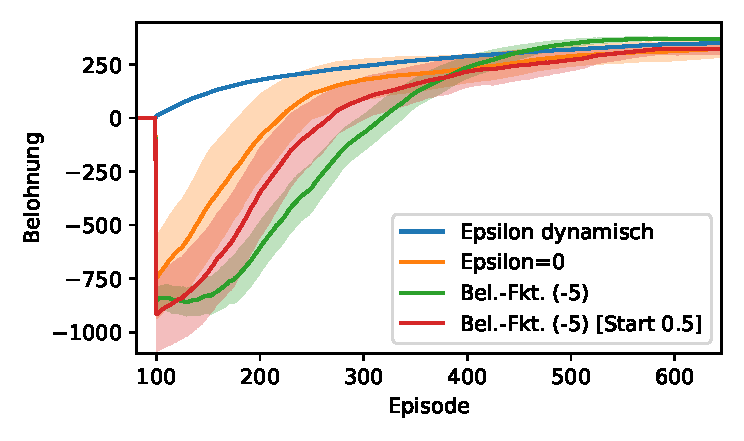
\includegraphics[width=\textwidth]{deep_q_learning/figure_mean_eps_5_in_rew_big.pdf}
        \caption{Ausschnitt des linken Startbereichs}
        \label{img:graphEps5InRewBig}
    \end{subfigure}
    \begin{subfigure}[b]{0.49\textwidth}
        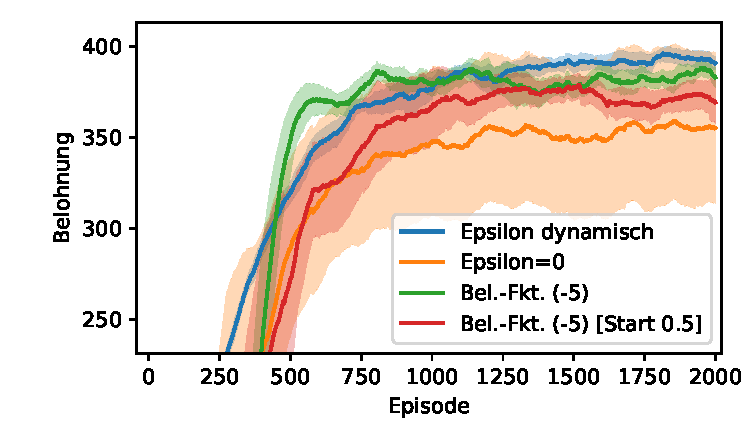
\includegraphics[width=\textwidth]{deep_q_learning/figure_mean_eps_5_in_rew_big2.pdf}
        \caption{Ausschnitt des oberen Bereichs}
        \label{img:graphEps5InRewBig2}
    \end{subfigure}
    \begin{subfigure}[b]{0.7\textwidth}
        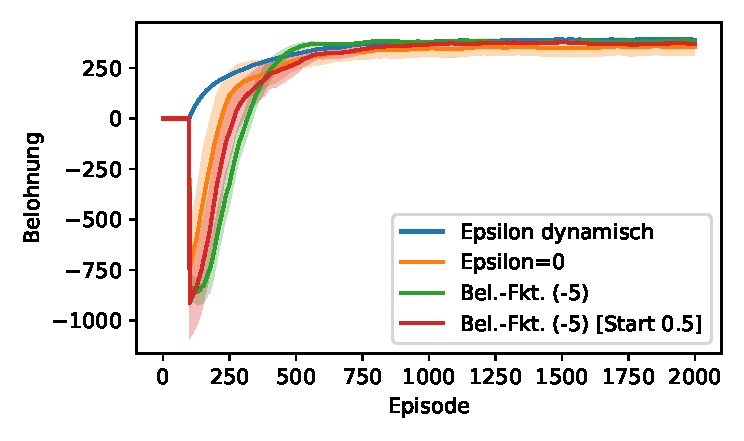
\includegraphics[width=\textwidth]{deep_q_learning/figure_mean_eps_5_in_rew.pdf}
        \caption{Kompletter Plot}
        \label{img:graphEps5InRew}
    \end{subfigure}
    \caption{Graph so wie in Abbildung \ref{img:graphQEpsComp}. Vergleich der Trainingsverläufe mit dynamischem $ \epsilon $ (blau), statischem $ \epsilon = 0.0 $ (gelb), modifiziertem Reward mit Faktor 5 (grün) und modifiziertem Reward mit Faktor 5 mit \mintinline{python}{start_exploration_rate=0.5} (rot) nach jeweils 20 Wiederholungen.}
    \label{img:graphEps5InRewBoth}
\end{figure} 

Die Graphen in Abbildung \ref{img:graphEps5InRewBoth} zeigen wieder den durchschnittlichen moving average und dessen Standardabweichung für alle Episoden. Zum Vergleich sind hier noch die Werte für das klassische Epsilon (blau) und dem fixen Epsilon 0.0 (orange) eingetragen. Der Graph in Abbildung \ref{img:graphEps5InRew} enthält alle Werte. Der Graph in Abbildung \ref{img:graphEps5InRewBig} zeigt für einen detaillierten Vergleich des ersten Trainingsviertels die ersten 600 Episoden. Um die Unterschiede nach dem ersten Trainingsviertel besser erkennen zu können, zeigt der Graph in Abbildung \ref{img:graphEps5InRewBig2} einen Ausschnitt der Belohnungswerte von 250 bis 400.

Die grüne und die rote Linie zeigt den Trainingsverlauf unter Anwendung oder oben beschriebenen, modifizierten Reward-Funktion, wobei letztere das Experiment mit\linebreak\mintinline{python}{start_exploration_rate=0.5} und \mintinline{python}{max_exploration_rate=0.5} beschreibt. Beide liefern im ersten Viertel des Trainings schlechtere Belohnungswerte als das Training ohne Erkundungsstrategie. Danach überholen sie dieses allerdings und liegen am Ende zwischen dem Training mit Epsilon=0 und der klassischen $ \epsilon $-greedy Strategie. Zudem scheinen die Ergebnisse zuverlässiger zu sein als bei Epsilon=0, wie man an der geringeren Standardabweichung -- vor allem gegen Ende -- erkennen kann.

Der Start mit einer geringeren \mintinline{python}{start_exploration_rate} führt wie erwartet am Anfang zu schnelleren Ergebnissen, wird allerdings von der Strategie, bei der die\linebreak\mintinline{python}{exploratrion_rate} bei 1 startet, überholt und scheint insgesamt etwas inkonsistentere Belohnungen zu liefern, was uns die Standardabweichung verrät.

Um zu beurteilen, wie sich der Agent nach dem Training verhält, sehen wir uns wieder die Boxplots an.

\begin{figure}[h!]
    \centering
    \begin{subfigure}[b]{0.7\textwidth}
        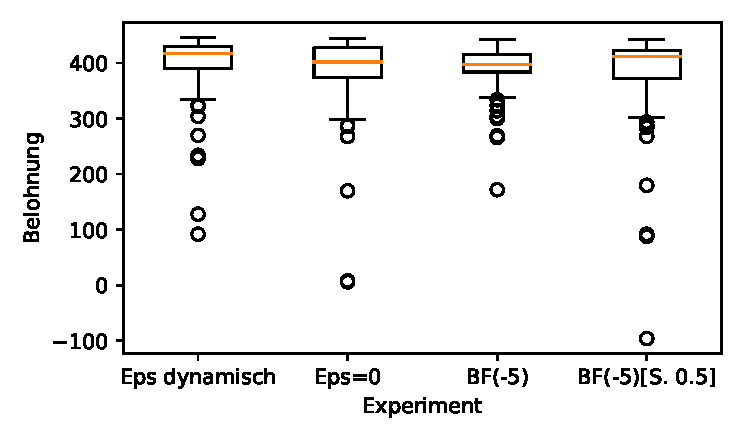
\includegraphics[width=\textwidth]{deep_q_learning/figure_box_eps_5_in_rew.pdf}
        \caption{Kompletter Plot}
        \label{img:graphBoxEps5InRew}
    \end{subfigure}
    \begin{subfigure}[b]{0.7\textwidth}
        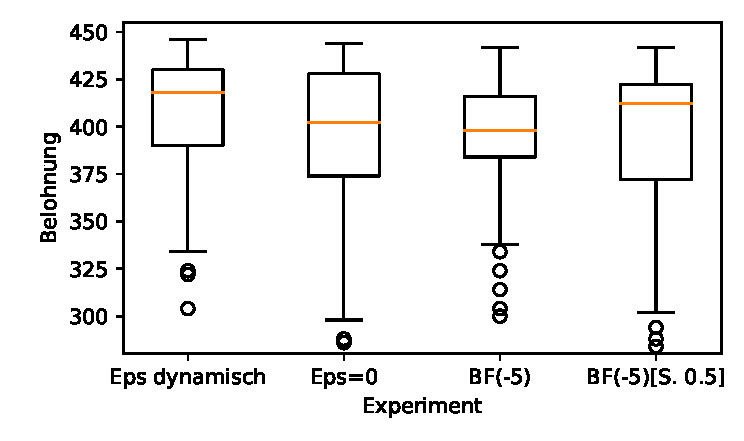
\includegraphics[width=\textwidth]{deep_q_learning/figure_box_eps_5_in_rew_big.pdf}
        \caption{Ausschnitt ohne die unteren Ausreißer}
        \label{img:graphBoxEps5InRewBig}
    \end{subfigure}
    \caption{Boxplots so wie in Abbildung \ref{img:graphBoxEpsComparisonBoth}. Experimente von links nach rechts: $ \epsilon $ dynamisch, $ \epsilon = 0.0 $, modifizierter Reward mit Faktor 5, modifizierter Reward mit Faktor 5 mit \mintinline{python}{start_exploration_rate=0.5}}
    \label{img:graphBoxEps5InRewBoth}
\end{figure}

Die Graphen in Abbildung \ref{img:graphBoxEps5InRewBoth} sind genauso aufgebaut wie die in Abbildung \ref{img:graphBoxEpsComparisonBoth}. Vergleichen wir nun die beiden Experimente mit der modifizierten Reward-Funktion miteinander. BF(-5) zeigt die Belohnungen mit der \mintinline{python}{start_exploration_rate=1}, BF(-5)[S. 0.5] beschreibt dementsprechend die Versuche mit \mintinline{python}{start_exploration_rate=0.5}. Bei letzterem liegt der Median etwas höher. Dies ist vermutlich wieder darauf zurückzuführen, dass die erkundeten Pfade aufgrund der niedrigen \mintinline{python}{exploration_rate} öfter durchlaufen wurden und für diese eine optimalere Strategie gefunden wurde. Allerdings ist das Minimum hier wieder niedriger. Wir denken auch hier, dass dies an der geringeren Quantität der durchlaufenen Pfade liegt und der Agent so für weniger Zustände eine Strategie entwickelt hat. Der Interquartilsabstand spiegelt gewissermaßen die Standardabweichung aus Abbildung \ref{img:graphEps5InRewBoth} wider. Der Agent mit \mintinline{python}{start_exploration_rate=1} liefert konsistentere Resultate. Sein Boxplot deckt zudem in Bezug auf Minimum und Maximum einen ähnlichen Bereich ab wie die des klassischen $ \epsilon $-greedy Agenten. Die Quartile von letzterem liegen allerdings weiterhin weiter oben, was dessen höheren moving average am Ende vom Graph in Abbildung \ref{img:graphEps5InRewBig2} erklärt.

\paragraph{Modifizierter Reward mit zufälligem Faktor}
Wir wollen nun versuchen, den Schwerpunkt noch etwas mehr auf die zufällige Erkundung der Umgebung zu setzen. Wir passen hierfür unsere Belohnungs-Funktion an:
\begin{minted}{python}
modified_reward = (1 - exploration_rate) * reward -\
                  exploration_rate * random.uniform(0.0, 5.0)
\end{minted}
Die \mintinline{python}{exploration_rate} wird nun nicht mehr direkt mit unserem errechneten Wert 5 multipliziert, sondern mit einem zufälligen Wert zwischen 0 und 5. Dies soll die zufällige Wahl der Aktionen und damit die zufällige Erkundung der Umgebung gewissermaßen über die Belohnung abbilden. Wir belassen es diesmal bei einem Experiment mit \mintinline{python}{start_exploration_rate=1} und \mintinline{python}{max_exploration_rate=1}, da diese Parameter im letzten Experiment konsistentere Werte und ein höheres Endergebnis geliefert haben. Wir vergleichen das Resultat wieder mit der klassischen $ \epsilon $-greedy Strategie (blau) und dem fixen Epsilon 0.0 (orange). Außerdem plotten wir das Resultat des letzten Experiments mit\linebreak\mintinline{python}{start_exploration_rate=1} (grün). Wir stellen diese Daten so wie in Abbildung \ref{img:graphEps5InRewBoth} dar.

\begin{figure}[h!]
    \centering
    \begin{subfigure}[b]{0.49\textwidth}
        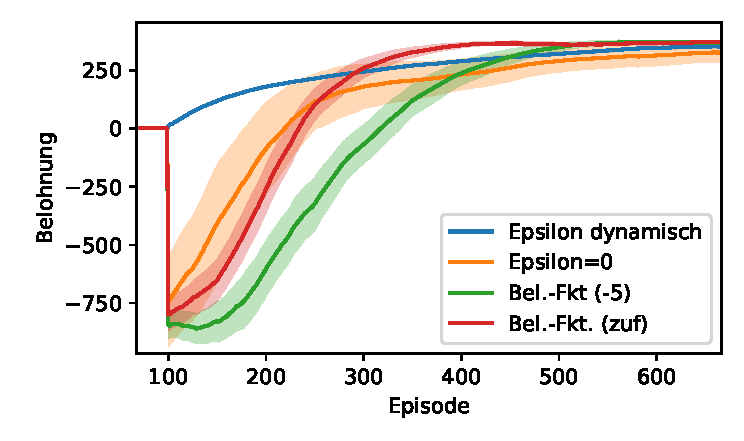
\includegraphics[width=\textwidth]{deep_q_learning/figure_mean_eps_rand_vs_5_in_rew_big.pdf}
        \caption{Ausschnitt des linken Startbereichs}
        \label{img:graphEpsRandVs5InRewBig}
    \end{subfigure}
    \begin{subfigure}[b]{0.49\textwidth}
        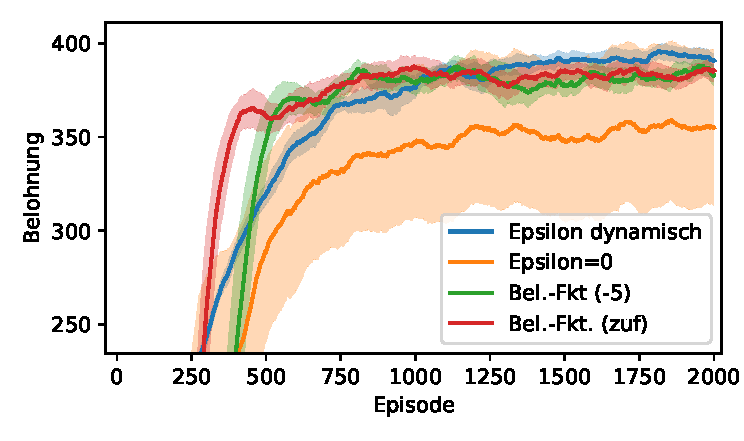
\includegraphics[width=\textwidth]{deep_q_learning/figure_mean_eps_rand_vs_5_in_rew_big2.pdf}
        \caption{Ausschnitt des oberen Bereichs}
        \label{img:graphEpsRandVs5InRewBig2}
    \end{subfigure}
    \begin{subfigure}[b]{0.7\textwidth}
        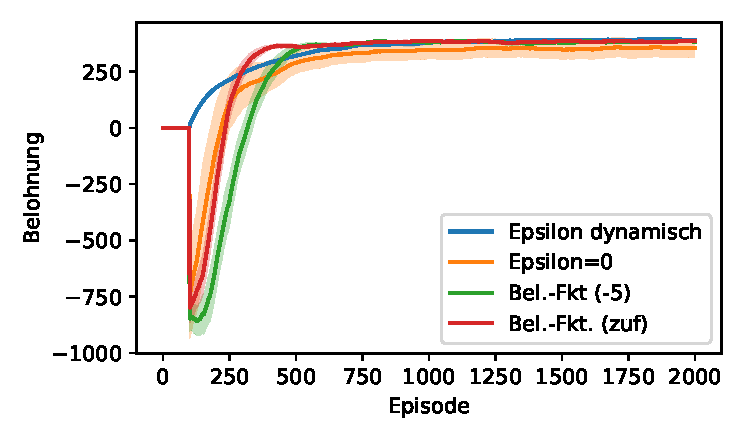
\includegraphics[width=\textwidth]{deep_q_learning/figure_mean_eps_rand_vs_5_in_rew.pdf}
        \caption{Kompletter Plot}
        \label{img:graphEpsRandVs5InRew}
    \end{subfigure}
    \caption{Graph so wie in \ref{img:graphQEpsComp}. Vergleich der Trainingsverläufe mit dynamischem $ \epsilon $ (blau), statischem $ \epsilon = 0.0 $ (gelb), modifiziertem Reward mit Faktor 5 (grün) und modifiziertem Reward mit Faktor zufällig zwischen 0 und 5 (rot) nach jeweils 20 Wiederholungen.}
    \label{img:graphEpsRandVs5InRewBoth}
\end{figure}

Die Daten des neuen Experiments sind in Abbildung \ref{img:graphEpsRandVs5InRewBoth} rot eingezeichnet. Die Form der Kurve dessen ist ähnlich mit der des vorangegangenen Experiments, allerdings verläuft sie leicht höher, gut erkennbar in Abbildung \ref{img:graphEpsRandVs5InRewBig}. Eine weitere Ähnlichkeit ist der Belohnungswert, bei dem sich beide gegen Ende des Trainings einpendeln, wie in Abbildung \ref{img:graphEpsRandVs5InRewBig2} zu sehen ist. Allerdings kommt der Agent mit dem Zufallsfaktor in seiner Belohnung etwas schneller bei diesem Wert an, was als eine direkte Verbesserung zum letzten Experiment angesehen werden kann. Im Punkt der Konsistenz stimmen die Experimente augenscheinlich ebenfalls überein, da sich die Standardabweichung der beiden kaum unterscheidet.

Beide liegen dementsprechend am Ende über dem Wert des Trainings ohne Erkundungsstrategie, allerdings weiterhin unter der klassischen $ \epsilon $-greedy Strategie.

Betrachten wir auch für diesen Vergleich die Boxplots der Experimente.
\begin{figure}[h!]
    \centering
    \begin{subfigure}[b]{0.7\textwidth}
        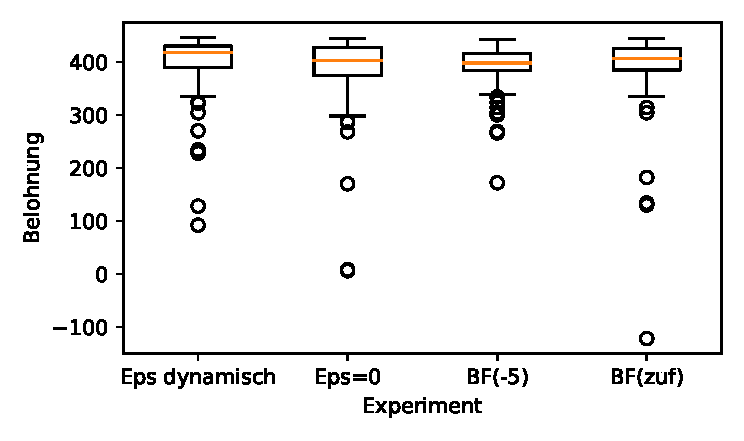
\includegraphics[width=\textwidth]{deep_q_learning/figure_box_eps_rand_vs_5_in_rew.pdf}
        \caption{Kompletter Plot}
        \label{img:graphBoxEpsRandVs5InRew}
    \end{subfigure}
    \begin{subfigure}[b]{0.7\textwidth}
        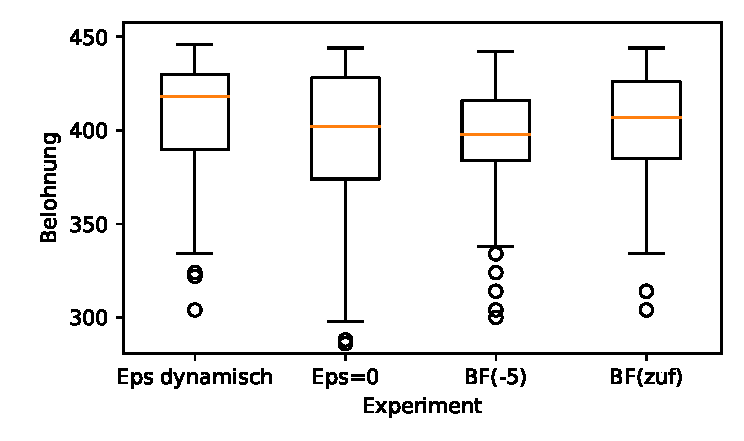
\includegraphics[width=\textwidth]{deep_q_learning/figure_box_eps_rand_vs_5_in_rew_big.pdf}
        \caption{Ausschnitt ohne die unteren Ausreißer}
        \label{img:graphBoxEpsRandVs5InRewBig}
    \end{subfigure}
    \caption{Boxplots so wie in Abbildung \ref{img:graphBoxEpsComparisonBoth}. Experimente von links nach rechts: $ \epsilon $ dynamisch, $ \epsilon = 0.0 $, modifizierter Reward mit Faktor 5, modifizierter Reward mit Faktor zufällig zwischen 0 und 5}
    \label{img:graphBoxEpsRandVs5InRewBoth}
\end{figure}
Die Graphen in Abbildung \ref{img:graphBoxEpsRandVs5InRewBoth} sind genauso aufgebaut wie in Abbildung \ref{img:graphBoxEps5InRewBoth}. Auch hier lässt sich erkennen, dass sich die Boxplots der beiden Agenten mit modifizierter Belohnungs-Funktion sehr ähneln. Lediglich der Median vom neuen Experiment (BF(zuf)) ist ein wenig höher als der des letzten Versuchs (BF(-5)). Das Resultat des neuen Experiments ist zudem schon sehr ähnlich zu dem des klassischen $ \epsilon $-greedy Agenten (Eps dynamisch). Auch hier scheint nur der Median weiter oben zu liegen. Im Vergleich zu dem des Agenten ohne Erkundungsstrategie liegt vor allem das Minimum aller anderen Experimente ein gutes Stück höher.

\paragraph{Modifizierter Reward mit Faktor 0}
Wir haben im letzten Experiment gesehen, dass das Austauschen des fixen Multiplikators 5 in der Belohnungs-Funktion mit einem zufälligen Wert zwischen 0 und 5 ein schnelleres Ergebnis liefert. Dies könnte bedeuten, dass Faktoren kleiner als 5 grundsätzlich besser funktionieren. Wir werden daher für unser nächstes Experiment diesen Faktor auf 0 setzen:
\begin{minted}{python}
modified_reward = (1 - exploration_rate) * reward - exploration_rate * 0
\end{minted}
Daher bleibt lediglich der reduzierte Wert der ursprünglichen Belohnung übrig:
\begin{minted}{python}
modified_reward = (1 - exploration_rate) * reward
\end{minted}
Wir betrachten erneut die durchschnittliche Belohnung der $ \epsilon $-greedy Strategie, Epsilon=0, die des letzten Experiments und natürlich die des aktuellen Experiments.
\begin{figure}[h!]
    \centering
    \begin{subfigure}[b]{0.49\textwidth}
        \includegraphics[width=\textwidth]{deep_q_learning/figure_mean_eps_0_vs_rand_in_rew_big.pdf}
        \caption{Ausschnitt des linken Startbereichs}
        \label{img:graphEps0VsRandInRewBig}
    \end{subfigure}
    \begin{subfigure}[b]{0.49\textwidth}
        \includegraphics[width=\textwidth]{deep_q_learning/figure_mean_eps_0_vs_rand_in_rew_big2.pdf}
        \caption{Ausschnitt des oberen Bereichs}
        \label{img:graphEps0VsRandInRewBig2}
    \end{subfigure}
    \begin{subfigure}[b]{0.7\textwidth}
        \includegraphics[width=\textwidth]{deep_q_learning/figure_mean_eps_0_vs_rand_in_rew.pdf}
        \caption{Kompletter Plot}
        \label{img:graphEps0VsRandInRew}
    \end{subfigure}
    \caption{Graph so wie in Abbildung \ref{img:graphQEpsComp}. Vergleich der Trainingsverläufe mit dynamischem $ \epsilon $ (blau), statischem $ \epsilon = 0.0 $ (gelb), modifiziertem Reward mit Faktor 0 (grün) und modifiziertem Reward mit Faktor zufällig zwischen 0 und 5 (rot) nach jeweils 20 Wiederholungen.}
    \label{img:graphEps0VsRandInRewBoth}
\end{figure}
Abbildung \ref{img:graphEps0VsRandInRewBoth} ist hierbei wieder ebenso aufgebaut wie Abbildung \ref{img:graphEps5InRewBoth}. In Abbildung \ref{img:graphEps0VsRandInRewBig} fällt auf, dass die Kurve des Experiments ohne zusätzlichen Faktor (Bel.-Fkt. (0)) zu Beginn schneller steigt als die mit zufälligem Faktor und auch die ohne Erkundungsstrategie. Der Graph in Abbildung \ref{img:graphEps0VsRandInRewBig2} zeigt uns, dass sie circa ab Episode 270 sehr ähnlich zu der des Experiments mit zufälligem Faktor in der Belohnung verläuft. Es lässt sich also festhalten, dass die Strategie dieses Experiments am Anfang des Trainings etwas schneller ist als unsere bisherigen Ansätze.

Sehen wir uns nun noch die Boxplots zu diesem Experiment an.
\begin{figure}[h!]
    \centering
    \begin{subfigure}[b]{0.7\textwidth}
        \includegraphics[width=\textwidth]{deep_q_learning/figure_box_eps_0_vs_rand_in_rew.pdf}
        \caption{Kompletter Plot}
        \label{img:graphBoxEps0VsRandInRew}
    \end{subfigure}
    \begin{subfigure}[b]{0.7\textwidth}
        \includegraphics[width=\textwidth]{deep_q_learning/figure_box_eps_0_vs_rand_in_rew_big.pdf}
        \caption{Ausschnitt ohne die unteren Ausreißer}
        \label{img:graphBoxEps0VsRandInRewBig}
    \end{subfigure}
    \caption{Boxplots so wie in Abbildung \ref{img:graphBoxEpsComparisonBoth}. Experimente von links nach rechts: $ \epsilon $ dynamisch, $ \epsilon = 0.0 $, modifizierter Reward mit Faktor 0, modifizierter Reward mit Faktor zufällig zwischen 0 und 5.}
    \label{img:graphBoxEps0VsRandInRewBoth}
\end{figure}
Abbildung \ref{img:graphBoxEps0VsRandInRewBoth} ist hier wieder so aufgebaut wie Abbildung \ref{img:graphBoxEps5InRewBoth}. Im Graphen in Abbildung \ref{img:graphBoxEps0VsRandInRewBig} sieht man, dass das neue Minimum (BF(0)) im Vergleich zum letzten Experiment (BF(zuf)) wieder etwas tiefer liegt. Allerdings ist dafür der Median größer und augenscheinlich fast auf einer Ebene mit dem des klassischen Ansatzes (Eps dynamisch). Außerdem zeigt der Graph in Abbildung \ref{img:graphBoxEps0VsRandInRew}, dass wir mit dem neuesten Ansatz am wenigsten Ausreißer haben. Dieser Faktor ist eventuell nicht sehr wichtig, fällt aber im Vergleich zu allen anderen bisherigen Boxplots doch auf. Eventuell gleicht diese Tatsache auch zusammen mit dem größeren Median das geringere Minimum aus. Dafür spricht die Beobachtung aus Abbildung \ref{img:graphEps0VsRandInRewBig2}, dass sich der Verlauf sowie die Standardabweichung der beiden Experimente sehr ähneln.

Aufgrund dessen und vor allem aufgrund der besseren Ergebnisse zu Beginn des Trainings, welche diesmal merklich über denen des Agenten ohne Erkundungsstrategie liegen, kommen wir zu dem Schluss, dass dies für diese Domäne unser bester Ansatz für die Abbildung einer Erkundungsstrategie im Reward ist. Der Agent lernt schneller, konsistenter und besser als ohne eine Erkundungsstrategie und die Lernresultate können sich laut Boxplots sogar fast mit denen der $ \epsilon $-greedy-Strategie messen.
    \chapter{Luna-Lander}\label{sec:LunaLander}
    \chapter{Related Work} \label{sec:relatedWork}
Das Entwickeln von alternativen Erkundungsstrategien stellt für viele Forscher ein interessantes Gebiet dar. Bisher gibt es noch keinen Ansatz, der eine Erkundungsstrategie nur durch die Modifikation des Rewards während des Trainings implementiert. Es existieren allerdings ein paar ähnliche Strategien:

In \cite{r09_csimcsek2006intrinsic} wird für die optimale Erkundung der Umgebung ein eigener Markov Decision Process (MDP) formuliert, der sogenannte \textit{derived MDP}. Wenn der Agent nach der optimalen Policy des derived MDPs agiert, führt er eine für das Erlernen einer optimalen Policy für den eigentlichen MDP optimale Erkundung der Umgebung aus. Abbildung \ref{img:rwIntrinsicReward} zeigt eine schematische Repräsentation des Algorithmus. Der externe Zustand sowie die Belohnung, welche von der Umgebung zurückgegeben werden, werden wie gewohnt für das Aktualisieren der Task Value Function des MDPs, also die der eigentlichen Aufgabe, verwendet. Die Wahl der Aktion hängt allerdings von der Behavior Value Function, also der des derived MDPs, ab. Diese nutzt einen intrinsischen Reward, welcher von der Entwicklung der Task Value Function abhängt.
\begin{figure}[h!]
    \centering
    \includegraphics[width=0.5\textwidth]{rw_intrinsic_reward.JPG}
    \caption{Schematische Repräsentation des Algorithmus} \label{img:rwIntrinsicReward}
    \source{\cite{r09_csimcsek2006intrinsic}}
\end{figure}
Hier wird also neben der externen Belohnung eine hiervon abhängige weitere Belohnung erzeugt, welche Auswirkungen auf das Lernverhalten des Agenten hat. Es lässt sich argumentieren, dass diese zweite Belohnung Ähnlichkeiten mit unserer modifizierten Belohnung hat.

Das Konzept von intrinsischen Rewards ist natürlich nicht neu. Der bekannte KI-Forscher Jürgen Schmidhuber erklärt in \cite{r01_schmidhuber2009driven}, dass \textit{curiosity} dazu genutzt werden kann, den Agenten zur aktiven Erkundung der Umgebung anzuregen. Der Agent soll hierfür die beobachteten Daten aufgrund von auftretenden Regularitäten zusammenzufassen. Die komprimierte Version der Daten kann als deren vereinfachte Erklärung aufgefasst werden. Daten, welche sich nicht in bisher bekannte Regelmäßigkeiten einordnen lassen, sollen für den Agenten interessanter sein, da diese zum Erlernen einer besseren Komprimierung aller Daten beitragen. Deshalb erhält der Agent zusätzlich einen internen Reward, wenn er lernt die bisher gesammelten Daten mit weniger Bits darzustellen, welcher zusammen mit dem externen Reward maximiert werden soll. Diese Methode soll auch in Umgebungen mit spärlicher Belohnung dazu führen, dass der Agent diese erkundet und lernt wie sie funktioniert. Dieser intrinsische Reward, welchen Schmidhuber als \textit{curiosity reward} bezeichnet, hat also ebenfalls starke Auswirkung auf das Erkundungs- und Lernverhalten, weswegen wir diesen Ansatz hier erwähnen.

Im Gegensatz zu unserer Idee, den Reward in Bezug auf $ \epsilon $ zu modifizieren, existiert außerdem der gegenteilige Ansatz, den Wert von $ \epsilon $ während des Trainings je nach erhaltenem Reward zu kontrollieren. \cite{r13_dos2017adaptive} nennt dies \textit{adaptive $ \epsilon $-greedy} und geht hierbei so vor, dass nach einer gewissen Anzahl von zufällig gewählten Aktionen überprüft wird, ob die durchschnittliche Belohnung größer ist als beim letzten Mal. Falls ja wird $ \epsilon $ entsprechend angepasst, ist sie geringer, so wird $ \epsilon $ aus 0.5 gesetzt. In Abbildung \ref{img:rwAdaptiveEpsilon} ist diesen Algorithmus dargestellt. 
\begin{figure}[h!]
    \centering
    \includegraphics[width=\textwidth]{rw_adaptive_epsilon.JPG}
    \caption{Adaptiver $ \epsilon $-greedy-Algorithmus} \label{img:rwAdaptiveEpsilon}
    \source{\cite{r13_dos2017adaptive}}
\end{figure}
\cite{r13_dos2017adaptive} zeigt, dass die adaptive $ \epsilon $-greedy-Methode in den durchgeführten Experimenten zu besseren Ergebnissen führt als die $ \epsilon $-greedy Methode. Man muss allerdings erwähnen, dass das $ \epsilon $ bei letzterem einen statischen Wert hat.

Eine weitere Lernmethode, die ohne einen Reward auskommt, ist das in \cite{r02_eysenbach2018diversity} beschriebene Erlernen von Fähigkeiten mittels \textit{Diversity}. In einer unüberwachten Phase soll der Agent zunächst eine Menge von Fähigkeiten erlernen, die sich stark voneinander unterscheiden. Hierzu folgt der Agent dem DIAYN-Algorithmus (\glqq Diversity is all you need\grqq{}). Die Belohnung für die einzelnen Aktionen hängt in dieser Phase von der Unterscheidbarkeit der Fähigkeiten ab. Anders gesagt sollen sich die besuchten Zustände so unterschiedlich wie möglich sein.
\begin{figure}[h!]
    \centering
    \includegraphics[width=0.4\textwidth]{rw_curiosity.JPG}
    \caption{Mittels DIAYN erlernte Skills in einem 2D-Environment} \label{img:rwCuriosity}
    \source{\cite{r02_eysenbach2018diversity}}
\end{figure}
In Abbildung \ref{img:rwCuriosity} ist das Ergebnis dieser Phase für eine simple 2D Navigation dargestellt. Der Agent startet hier in der Mitte und kann sich im Raum bewegen. Es lässt sich erkennen, dass die erlernten Fähigkeiten, welche hier als farbige Pfade dargestellt sind, aufgrund ihrer Ungleichheit einen Großteil des Zustandsraums abdecken. Wenn nun die Aufgabe in der nächsten Phase lautet, dass der Agent nach unten links gehen soll, so ist der lila Pfad ein sehr vielversprechender Kandidat. Die Tatsache, dass die erlernten Fähigkeiten im Idealfall so unterschiedlich wie möglich sind, stellt nach \cite{r02_eysenbach2018diversity} sicher, dass einige brauchbare Fähigkeiten dabei sind. Soll der Agent nun ein tatsächliches Problem in der Domäne lösen, werden die gefundenen Fähigkeiten als mögliche Aktionen genutzt. \cite{r02_eysenbach2018diversity} zeigt anhand von einigen Experimenten, dass die DIAYN-Methode zu schnelleren Lernerfolgen führt. 
    \chapter{Ergebnisse und Fazit} \label{sec:conclusion}
%% EINSTIEG
% Reward hat (große) Auswirkung auf das Lernverhalten
% Durch Veränderung des Rewards haben wir das Ziel des Agtenten verändert
% Wir konnten zeigen, dass unser Ansatz eine Daseinsberechtigung hat
Der Reward ist die zentrale Komponente beim Reinforcement Learning. Wir konnten durch die Experimente in dieser Arbeit ein Gefühl dafür entwickeln, inwieweit er sich für die Abbildung einer Erkundungsstrategie eignet.

%% ZUSAMMENFASSUNG
Zu Beginn der Arbeit haben wir in Kapitel \ref{sec:basics} die Grundlagen von Q-Learning und Deep-Q-Learning, sowie Exploration und Exploitation erklärt. Auf dieser Basis haben wir im Anschluss in Kapitel \ref{sec:NavigationProblem} auf unserer eigens für diese Arbeit entwickelten Domäne gezeigt, dass die Modifikation des Rewards beim Q-Learning eine größere durchschnittliche Belohnung erzielt als das Nichtbenutzen einer Erkundungsstrategie. Anschließend haben wir über die Änderung des Rewards, welcher von der Umgebung zurückgegeben wird, das Ziel des Agenten so angepasst, dass es für unsere Experimente mit Deep-Q-Learning geeignet ist. Wir sind hier zu dem Schluss gekommen, dass die Multiplikation des Rewards mit dem Faktor \mintinline{python}{(1 - exploration_rate)} sowohl in Hinblick auf Trainingsverlauf und -konsistenz als auch auf das Resultat einen Vorteil gegenüber einem Agenten ohne Erkundungsstrategie bringt und sogar teilweise ähnlich gut performt wie $ \epsilon $-greedy. Die $ \epsilon $-greedy-Strategie war allerdings wie erwartet in beiden Fällen in jeder Hinsicht die beste Strategie. In Kapitel \ref{sec:LunaLander} haben wir die erarbeitete Strategie auf der Domäne des Lunar Landers getestet und konnten feststellen, dass unsere Strategie auch hier Potenzial besitzt. Die Unterschiede sind hier nicht so deutlich wie bei unserer Domäne, dennoch führt die Modifikation des Rewards zu einem im Großen und Ganzen besseren Ergebnis als beim Agenten ohne Erkundungsstrategie. Im Vergleich lernt unser Ansatz zu Beginn des Trainings etwas schneller und liefert etwas bessere Resultate, allerdings stürzt der durchschnittliche Belohnungswert während des Trainings bis unter den des Vergleichsagenten ab und die Standardabweichung bricht aus. Für ein eindeutiges Ergebnis sind auf dieser Domäne mehr Daten erforderlich. In Kapitel \ref{sec:relatedWork} haben wir verwandte Arbeiten und deren Vorgehen betrachtet. 

%% ERGEBNISSE
% Auf eigener Domäne besserer Trainingsverlauf und Ergebnis als keine Erkundungsstrategie sowohl beim Q-Learning als auch beim Deep-Q-Learning
Auf unserer eigenen Domäne hat sich somit gezeigt, dass der von uns erarbeitete Ansatz sowohl beim Q-Learning als auch beim Deep-Q-Learning bessere Ergebnisse liefert als ein Agent ohne Erkundungsstrategie. Die Trainingsresultate waren bei den Deep-Q-Learning-Experimenten sogar ähnlich gut wie bei der Verwendung der $ \epsilon $-greedy-Strategie. Beim Lunar Lander war das Ergebnis nicht ganz so eindeutig. Unsere Versuche haben zwar gezeigt, dass unsere Strategie auch hier das Training positiv beeinflusst, lässt aber einige Fragen offen. So ist beispielsweise unklar, warum der Belohnungsdurchschnitt nach seinem Höhepunkt wieder sehr stark abfällt. Um hier eine klare Aussage treffen zu können, benötigen wir mehr Daten, welche wir aufgrund des Mangels an nötigen Rechenressourcen im Zuge dieser Arbeit nicht erlangen konnten. 

%% SELBSTKRITIK
Wir sind uns außerdem darüber im Klaren, dass die 10 Iterationen beim Lunar Lander keine starke statistische Aussagekraft haben. Die Ergebnisse dieser Domäne stellen also eher eine Tendenz dar. Es steht ebenfalls fest, dass die erfolgreiche Anwendung in ein bis zwei Domänen nicht für das Funktionieren unserer Methode im Allgemeinen spricht.

%% FORSCHUNGSFRAGE
Wir konnten allerdings die zugrunde liegende Fragestellung dieser Arbeit, ob das Abbilden einer Erkundungsstrategie über den Reward eine Daseinsberechtigung hat, beantworten. Die gesammelten Ergebnisse zeigen, dass unser Ansatz dahingehend funktioniert, die Performance im Vergleich zu einem Trainieren ohne Erkundungsstrategie zu verbessern und er dementsprechend Potenzial hat. Wir haben Reward-Funktionen gefunden, die wir rein greedy lernen, die sich aber ähnlich verhalten wie $ \epsilon $-greedy und deren Lernverhalten trotz der Modifikation des Rewards eine sehr hohe Stabilität besitzen. Verlagert man möglichst viele Komponenten des Lernalgorithmus in die Reward-Funktion, so muss man am Ende nur deren Korrektheit überprüfen und läuft weniger Gefahr eine künstliche Intelligenz zu schaffen, die etwas anderes lernt als das, was wir vorgesehen haben. Im besten Fall haben wir so die Möglichkeit genau aufzuschreiben, was der Agent versucht zu tun.

%% AUSBLICK
% Mehr Daten bzgl. Lunar Lander
% Reaktives Anpassen des Rewards
Für eine weitere Forschungsarbeit wäre es interessant, unsere Strategie zum einen ausgiebiger auf der Domäne des Lunar Lander zu testen, um hier eine aussagekräftige Statistik erstellen zu können und die offenen Fragen zu klären. Zudem könnte man die Experimente auf weitere bekannte Domänen ausweiten und mit bisherigen Forschungsergebnissen vergleichen. Es wäre außerdem spannend zu erforschen, wie sich eine reaktive Modifikation des Rewards auf den Verlauf und die Resultate des Trainings auswirkt, die Anpassung der Belohnung also unter Berücksichtigung des aktuellen Zustands und des bisherigen Trainingsverlaufs stattfindet.
    % further chapters 
%
% =================================================================================================
% place your appendix here
% -------------------------------------------------------------------------------------------------
%
    % \appendix
    % % -------------------------------------------------------------------------------------------------
%      MDSG Latex Framework
%      ============================================================================================
%      File:                  appendix.tex
%      Author(s):             Michael Duerr
%      Version:               1
%      Creation Date:         30. Mai 2010
%      Creation Date:         30. Mai 2010
%
%      Notes:                 - Place your appendix here
%                             - Use the same commands (`chapter', `section', ...) as in main text
% -------------------------------------------------------------------------------------------------
%
\chapter{Beispiel Anhang}
\small{
\begin{verbatim}
/*
* This code serves the initialization of an auxiliary probability array.
* The array holds at each position a pre-calculated probability for the index
* of that position. The probability reflects the Zipf-distribution for the
* corresponding indexes
*/
Set zipfExponent to 1.4
Set sum to 0
Set maxInteger to 65535
FOR i = 0 to maxInteger
probArray[i] = 1/pow(i + 1, zipfExponent)
Set sum = sum + probArray[i]
END FOR
FOR i = 0 to maxInteger
Set probArray[i] = probArray[i]/sum
END FOR
FOR i = 1 to maxInteger
Set probArray[i] = probArray[i] + probArray[i] = probArray[i-1]
END FOR

/*
* This code gets called in case a Zipf-distributed number is required. It
* iterates over the probability array until the chosen random number v
* is less than the value stored at the current array position i. The value of
* the array position will be returned as the calculated Zipf-distributed
* number
*/
Set v to a random number between 0 and 1
FOR i = 0 to maxInteger
IF v < probArray[i] THEN
RETURN i
END IF
END FOR
RETURN 0

\end{verbatim}
}

    % further appendix
%
% =================================================================================================
% comment \listoffigures and/or \listoftables if not wanted
% -------------------------------------------------------------------------------------------------
%
    \backmatter
    \listoffigures                                % list of figures (uncomment if wanted)
    \listoftables                                 % list of tables (uncomment if wanted)
    \lstlistoflistings                            % list of listings (uncomment if wanted)
%
% =================================================================================================
% place your bibliography here
% -------------------------------------------------------------------------------------------------
%
    \begin{spacing}{0.9}                          % save some space
       \bibliographystyle{geralpha}               % for german thesis
    %    \bibliographystyle{chicago}
       %\bibliographystyle{alpha}                 % for english thesis
       \bibliography{bibliography}                % the location of bib file
    \end{spacing}
\end{document}
%
% =================================================================================================
% end of document
% -------------------------------------------------------------------------------------------------
%
